% This LaTeX document needs to be compiled with XeLaTeX.
\documentclass[10pt]{article}
\usepackage[utf8]{inputenc}
\usepackage{amsmath}
\usepackage{amsfonts}
\usepackage{amssymb}
\usepackage[version=4]{mhchem}
\usepackage{stmaryrd}
\usepackage{bbold}
\usepackage{graphicx}
\usepackage[export]{adjustbox}
\graphicspath{ {./images/} }
\usepackage[fallback]{xeCJK}
\usepackage{polyglossia}
\usepackage{fontspec}
\IfFontExistsTF{Noto Serif CJK TC}
{\setCJKmainfont{Noto Serif CJK TC}}
{\IfFontExistsTF{STSong}
  {\setCJKmainfont{STSong}}
  {\IfFontExistsTF{Droid Sans Fallback}
    {\setCJKmainfont{Droid Sans Fallback}}
    {\setCJKmainfont{SimSun}}
}}

\setmainlanguage{spanish}
\IfFontExistsTF{CMU Serif}
{\setmainfont{CMU Serif}}
{\IfFontExistsTF{DejaVu Sans}
  {\setmainfont{DejaVu Sans}}
  {\setmainfont{Georgia}}
}

\begin{document}
\section*{Enumeración}
Antes de comenzar recordaremos la definición del número combinatorio $\binom{\alpha}{k}$ para un número real $\alpha$ que necesitaremos más adelante.\\
Si $\alpha$ es un número real y $k$ es un entero no negativo, denotaremos por $(\alpha)_{k}$ al producto

$$
(\alpha)_{k}=\alpha(\alpha-1)(\alpha-2) \ldots . .(\alpha-k+1)
$$

Notemos que en el caso en que $\alpha=n$, con $n$ un entero no negativo, se tiene que

$$
(\alpha)_{k}=(n)_{k}=n(n-1)(n-2) \ldots(n-k+1)=\frac{n!}{(n-k)!}
$$

Luego, el número combinatorio $\binom{n}{k}$ puede escribirse en la forma $\binom{n}{k}=\frac{(n)_{k}}{k!}$. Esto sugiere extender la definición del número combinatorio al caso real de la siguiente manera:\\
Definición: Sea $\alpha$ un número real y sea $k$ un entero no negativo. Definimos el número combinatorio $\binom{\alpha}{k}$ en la forma

$$
\binom{\alpha}{k}=\frac{(\alpha)_{k}}{k!}
$$

Con esta definición se verifican:\\
i) Si $x \in \mathbb{R}$ y $|x|<1$ entonces $(1+x)^{\alpha}=\sum_{k=0}^{\infty}\binom{\alpha}{k} x^{k}$\\
ii) $(-1)^{k}\binom{-\alpha}{k}=\binom{\alpha+k-1}{k}$

\section*{1. Funciones generatrices.}
Los siguientes ejemplos muestran la utilidad de las funciones generatrices para contar. Más adelante, en la sección 5. veremos su aplicación en las relaciones de recurrencia.

Ejemplo 1. Supongamos que queremos determinar de cuántas maneras se pueden distribuir 4 bolillas indistinguibles en 3 cajas distintas, $a, b, c$, con la condición de que en la caja $a$ haya al menos 2 bolillas.\\
Las 6 soluciones de este problema pueden expresarse en la forma:\\
$a a b b$ (dos bolillas en la caja $a$ y dos en la caja $b$ )\\
aacc (dos bolillas en la caja $a$ y dos en la caja $c$ )\\
aabc (dos bolillas en la caja $a$, una en la $b$ y una en la $c$ )\\
aaab (tres bolillas en la caja $a$ y una en la $b$ )\\
aaac (tres bolillas en la caja $a$ y una en la $c$ )\\
aaaa (cuatro bolillas en la caja $a$ )

Como sabemos, esto es lo mismo que determinar la cantidad de soluciones enteras no negativas $e_{1}, e_{2}, e_{3}$ de la ecuación $e_{1}+e_{2}+e_{3}=4$ tales que $e_{1} \geq 2$.\\
Si consideramos la igualdad

$$
\left(x^{2}+x^{3}+x^{4}+\cdots\right) \cdot\left(x^{0}+x^{1}+x^{2}+\cdots\right) \cdot\left(x^{0}+x^{1}+x^{2}+\cdots\right)=\sum_{k \geq 0} c_{k} x^{k}
$$

aplicando la propiedad distributiva vemos que el coeficiente de $x^{k}$ en el miembro izquierdo es igual a la cantidad de productos $x^{e_{1}} x^{e_{2}} x^{e_{3}}$ tales que $e_{1}+e_{2}+e_{3}=k$ y $e_{1} \geq 2$. Luego, $c_{k}$ es igual a la cantidad de soluciones de $e_{1}+e_{2}+e_{3}=k$ tales que $e_{1} \geq 2$. Por lo tanto, la solución a nuestro problema es $c_{4}$.\\
Calculemos ahora $c_{4}$. Para ello, observemos que como $\sum_{j \geq 0} x^{j}=\frac{1}{1-x}$ entonces

$$
\begin{aligned}
& \left(x^{2}+x^{3}+x^{4}+\cdots\right) \cdot\left(x^{0}+x^{1}+x^{2}+\cdots\right) \cdot\left(x^{0}+x^{1}+x^{2}+\cdots\right)= \\
& =\frac{x^{2}}{(1-x)^{3}}=x^{2} \cdot(1-x)^{-3}=x^{2} \cdot \sum_{j \geq 0}\binom{-3}{j}(-x)^{j}= \\
& =\sum_{j \geq 0}\binom{3+j-1}{j} x^{j+2}=\sum_{k \geq 2}\binom{3+(k-2)-1}{k-2} x^{k}
\end{aligned}
$$

ya que

$$
\binom{-3}{j}=\frac{(-3)(-4) \ldots(-3-(j-1))}{j!}=(-1)^{j} \cdot \frac{3 \cdot 4 \ldots(3+j-1)}{j!}=\left(-1^{j}\right) \cdot\binom{3+j-1}{j}
$$

de donde $c_{4}=\binom{3+2-1}{2}=6$.\\
En general, hay $c_{k}=\binom{3+(k-2)-1}{k-2}$ maneras de distribuir k bolillas indistinguibles en 3 cajas distintas, con la condición de que la primera caja contenga al menos dos bolillas.\\
Definición: Dada una sucesión $\left(c_{k}\right)_{k \geq 0}$ de números reales, la serie de potencias $\sum_{k \geq 0} c_{k} x^{k}$ se llama la función generatriz de la sucesión ( $c_{k}$ ).

Ejemplo 2. Supongamos que queremos determinar de cuántas maneras se pueden distribuir 4 bolillas numeradas en 3 cajas numeradas, con la condición de que en la primera caja haya al menos 2 bolillas. Observemos que esto es lo mismo que contar cuántas funciones $f:\{1,2,3,4\} \longrightarrow\{a, b, c\}$ hay que satisfagan que $f(x)=a$ para al menos dos valores de $x$. Escribiendo $a b b a$ para indicar la función que satisface $f(1)=a, f(2)=b, f(3)=b$ y $f(4)=a$, abac para indicar la función que satisface $f(1)=a, f(2)=b, f(3)=a$ y $f(4)=c$, etc., resulta que todas las soluciones de este problema son:\\
$a a b b$ y todas sus permutaciones (esto cuenta todas las soluciones en las que hay dos bolillas en la caja $a$ y dos en la caja $b$ )\\
aacc y todas sus permutaciones (esto cuenta todas las soluciones en las que hay dos bolillas en la caja $a$ y dos en la caja $c$ )\\
aabc y todas sus permutaciones (soluciones con dos bolillas en la caja $a$, una en la $b$ y una en la $c$ )\\
aaab y todas sus permutaciones (soluciones con tres bolillas en la caja $a$ y una en la $b$ ) aaac y todas sus permutaciones (soluciones con tres bolillas en la caja $a$ y una en la $c$ ) aaaa y todas sus permutaciones (soluciones con cuatro bolillas en la caja $a$ ) Luego, la cantidad de soluciones es

$$
\frac{4!}{2!2!}+\frac{4!}{2!2!}+\frac{4!}{2!1!1!}+\frac{4!}{3!1!}+\frac{4!}{3!1!}+\frac{4!}{4!}
$$

Si consideramos ahora la igualdad

$$
\left(\frac{x^{2}}{2!}+\frac{x^{3}}{3!}+\frac{x^{4}}{4!}+\cdots\right) \cdot\left(\frac{x^{0}}{0!}+\frac{x^{1}}{1!}+\frac{x^{2}}{2!}+\cdots\right) \cdot\left(\frac{x^{0}}{0!}+\frac{x^{1}}{1!}+\frac{x^{2}}{2!}+\cdots\right)=\sum_{k \geq 0} c_{k} \frac{x^{k}}{k!}
$$

aplicando la propiedad distributiva vemos que el coeficiente de $x^{4}$ en el miembro izquierdo es igual a

$$
\frac{1}{2!2!}+\frac{1}{2!2!}+\frac{1}{2!1!1!}+\frac{1}{3!1!}+\frac{1}{3!1!}+\frac{1}{4!}
$$

Luego,

$$
\frac{c_{4}}{4!}=\frac{1}{2!2!}+\frac{1}{2!2!}+\frac{1}{2!1!1!}+\frac{1}{3!1!}+\frac{1}{3!1!}+\frac{1}{4!}
$$

de donde resulta que $c_{4}$ es la solución del problema:

$$
\frac{4!}{2!2!}+\frac{4!}{2!2!}+\frac{4!}{2!1!11!}+\frac{4!}{3!1!}+\frac{4!}{3!1!}+\frac{4!}{4!}=4!.\left(\frac{1}{2!2!}+\frac{1}{2!2!}+\frac{1}{2!1!1!}+\frac{1}{3!1!}+\frac{1}{3!1!}+\frac{1}{4!}\right)=c_{4}
$$

Veamos ahora cómo calcular $c_{4}$. Para ello observemos que $e^{x}=\sum_{k \geq 0} \frac{x^{k}}{k!}$, de donde

$$
\begin{aligned}
& \left(\frac{x^{2}}{2!}+\frac{x^{3}}{3!}+\frac{x^{4}}{4!}+\cdots\right) \cdot\left(\frac{x^{0}}{0!}+\frac{x^{1}}{1!}+\frac{x^{2}}{2!}+\cdots\right) \cdot\left(\frac{x^{0}}{0!}+\frac{x^{1}}{1!}+\frac{x^{2}}{2!}+\cdots\right)= \\
& =\left(e^{x}-1-x\right) \cdot e^{x} \cdot e^{x}=\left(e^{x}-1-x\right) \cdot e^{2 x}=e^{3 x}-e^{2 x}-x \cdot e^{2 x}= \\
& =\sum_{k \geq 0} 3^{k} \frac{x^{k}}{k!}-\sum_{k \geq 0} 2^{k} \frac{x^{k}}{k!}-x \sum_{k \geq 0} 2^{k} \frac{x^{k}}{k!}=\sum_{k \geq 0} 3^{k} \frac{x^{k}}{k!}-\sum_{k \geq 0} 2^{k} \frac{x^{k}}{k!}-\sum_{k \geq 0} 2^{k} \frac{x^{k+1}}{k!}= \\
& =\sum_{k \geq 0} 3^{k} \frac{x^{k}}{k!}-\sum_{k \geq 0} 2^{k} \frac{x^{k}}{k!}-\sum_{k \geq 0}(k+1) 2^{k} \frac{x^{k+1}}{(k+1)!}= \\
& =\sum_{k \geq 0} 3^{k} \frac{x^{k}}{k!}-\sum_{k \geq 0} 2^{k} \frac{x^{k}}{k!}-\sum_{k \geq 0} k \cdot 2^{k-1} \frac{x^{k}}{k!}=\sum_{k \geq 0}\left(3^{k}-2^{k}-k \cdot 2^{k-1}\right) \frac{x^{k}}{k!}
\end{aligned}
$$

de donde resulta que $c_{4}=3^{4}-2^{4}-4.2^{4-1}=33$\\
En general, hay $c_{k}=3^{k}-2^{k}-k .2^{k-1}$ maneras de distribuir k bolillas numeradas en 3 cajas distintas, con la condición de que la primera caja contenga al menos dos bolillas.

Definición: Dada una sucesión $\left(c_{k}\right)_{k \geq 0}$ de números reales, la serie $\sum_{k \geq 0} c_{k} \frac{x^{k}}{k!}$ se llama la función generatriz exponencial de la sucesión ( $c_{k}$ ).

Ejemplo 3. Supongamos que queremos determinar de cuántas maneras se pueden distribuir $k$ bolillas indistinguibles en $n$ cajas numeradas, con la condición de que en cada caja haya a lo sumo una bolilla. Observemos que esto es lo mismo que determinar cuántas soluciones enteras $e_{1}, e_{2}, \ldots, e_{n}$ tiene la ecuación $e_{1}+e_{2}+\cdots+e_{n}=k$ que satisfagan $0 \leq e_{i} \leq 1$ para todo $i$. Si ahora consideremos la igualdad

$$
(1+x)^{n}=\sum_{j=0}^{n}\binom{n}{j} x^{j}
$$

es decir, la igualdad

$$
\underbrace{\left(x^{0}+x^{1}\right) \cdot\left(x^{0}+x^{1}\right) \ldots\left(x^{0}+x^{1}\right)}_{n \text { factores }}=\sum_{j=0}^{n} c_{j} x^{j}
$$

donde $c_{j}=\binom{n}{j}$, resulta que el coeficiente de $x^{k}$ en el miembro izquierdo es igual a la cantidad de productos $x^{e_{1}} x^{e_{2}} \ldots x^{e_{n}}$ tales que $e_{1}+e_{2}+\cdots+e_{n}=k$ y $0 \leq e_{i} \leq 1$ para todo $i$. Luego, la cantidad de soluciones de $e_{1}+e_{2}+\cdots+e_{n}=k$ tales que $0 \leq e_{i} \leq 1$ para todo $i$ es igual a $c_{k}=\binom{n}{k}$.\\
Ejemplo 4. Supongamos que queremos determinar de cuántas maneras se pueden distribuir $k$ bolillas indistinguibles en $n$ cajas numeradas. Observemos que esto es igual que determinar cuántas soluciones enteras $e_{1}, e_{2}, \ldots, e_{n}$ tiene la ecuación $e_{1}+e_{2}+\cdots+e_{n}=k$. Si ahora consideremos la igualdad

$$
\left(1+x+x^{2}+\cdots\right)^{n}=\sum_{j \geq 0} c_{j} x^{j}
$$

es decir, la igualdad

$$
\underbrace{\left(x^{0}+x^{1}+x^{2}+\cdots\right) \cdot\left(x^{0}+x^{1}+x^{2}+\cdots\right) \ldots\left(x^{0}+x^{1}+x^{2}+\cdots\right)}_{n \text { factores }}=\sum_{j=0}^{n} c_{j} x^{j}
$$

resulta que el coeficiente de $x^{k}$ en el miembro izquierdo es igual a la cantidad de productos $x^{e_{1}} x^{e_{2}} \ldots x^{e_{n}}$ tales que $e_{1}+e_{2}+\cdots+e_{n}=k$. Luego, la cantidad de soluciones de la ecuación $e_{1}+e_{2}+\cdots+e_{n}=k$ es igual a $c_{k}$.\\
Ahora calculemos $c_{k}$. Como

$$
\begin{aligned}
& \left(1+x+x^{2}+\cdots\right)^{n}=\left(\frac{1}{1-x}\right)^{n}=(1-x)^{-n}= \\
& =\sum_{j \geq 0}\binom{-n}{j}(-x)^{j}=\sum_{j \geq 0}\binom{n+j-1}{j} x^{j}
\end{aligned}
$$

pues

$$
\begin{aligned}
& \binom{-n}{j}=\frac{(-n)(-n-1)(-n-2) \ldots(-n-(j-1))}{j!}= \\
& =(-1)^{j} \cdot \frac{n(n+1)(n+2) \ldots(n+j-1)}{j!}=(-1)^{j}\binom{n+j-1}{j}
\end{aligned}
$$

Luego, $c_{k}=\binom{n+k-1}{k}$, de donde la cantidad de maneras en se pueden distribuir $k$ bolillas indistinguibles en $n$ cajas numeradas es igual a $\binom{n+k-1}{k}$.

Ejemplo 5. Supongamos que queremos determinar de cuántas maneras se pueden distribuir $k$ bolillas numeradas en $n$ cajas distintas. En este caso el problema se puede resolverse viendo que si $\left(\frac{x^{0}}{0!}+\frac{x^{1}}{1!}+\frac{x^{2}}{2!}+\cdots\right)^{n}=\sum_{j \geq 0} c_{j} \frac{x^{j}}{j!}$ entonces la cantidad de maneras de distribuir las bolillas es $c_{k}$, y usando que

$$
\left(\frac{x^{0}}{0!}+\frac{x^{1}}{1!}+\frac{x^{2}}{2!}+\frac{x^{3}}{3!}+\cdots\right)^{n}=e^{n x}=\sum_{j \geq 0} n^{j} \frac{x^{j}}{j!}
$$

Luego, la cantidad de maneras en que se pueden distribuir $k$ bolillas numeradas en $n$ cajas distintas es $n^{k}$.

Ejemplo 6. Supongamos que queremos determinar de cuántas maneras se pueden distribuir $n$ bolillas indistinguibles en $k$ cajas numeradas, con la condición de que en cada caja haya por lo menos una bolilla. Ahora el problema se puede resolverse viendo que es equivalente a calcular el coeficiente de $x^{n}$ de $\left(x+x^{2}+x^{3}+\cdots\right)^{k}$ y usando que

$$
\begin{aligned}
& \left(x+x^{2}+x^{3}+\cdots\right)^{k}=\left(\frac{x}{1-x}\right)^{k}=x^{k} \cdot(1-x)^{-k}=x^{k} \sum_{j \geq 0}\binom{k+j-1}{j} x^{j}= \\
& =\sum_{j \geq 0}\binom{k+j-1}{j} x^{j+k}=\sum_{j \geq k}\binom{j-1}{j-k} x^{j}=\sum_{j \geq k}\binom{j-1}{k-1} x^{j}
\end{aligned}
$$

resulta que la respuesta es $\binom{n-1}{k-1}$.\\
Ejemplo 7. Supongamos que queremos determinar de cuántas maneras se pueden distribuir $n$ bolillas numeradas en $k$ cajas distintas, con la condición de que en cada caja haya por lo menos una bolilla. Esto es lo mismo que determinar cuántas funciones de un conjunto de $n$ elementos en un conjunto de $k$ elementos hay que sean suryectivas. Llamaremos a este número $F(n, k)$ y en la sección 2 . volveremos a calcularlo de otra manera.

Observando que si $\left(\frac{x}{1!}+\frac{x^{2}}{2!}+\frac{x^{3}}{3!}+\cdots\right)^{k}=\sum_{j \geq 0} c_{j} \frac{x^{j}}{j!}$ entonces $F(n, k)=c_{n}$ y que

$$
\begin{aligned}
& \left(\frac{x}{1!}+\frac{x^{2}}{2!}+\frac{x^{3}}{3!}+\cdots\right)^{k}=\left(e^{x}-1\right)^{k}=\sum_{j=0}^{k}\binom{k}{j}\left(e^{x}\right)^{j}(-1)^{k-j}= \\
& =\sum_{j=0}^{k}\binom{k}{j}(-1)^{k-j} e^{j x}=\sum_{j=0}^{k}\binom{k}{j}(-1)^{k-j} \sum_{r \geq 0} j^{r} \frac{x^{r}}{r!}=\sum_{r \geq 0}\left(\sum_{j=0}^{k}\binom{k}{j}(-1)^{k-j} j^{r}\right) \frac{x^{r}}{r!}
\end{aligned}
$$

resulta que

$$
F(n, k)=\sum_{j=0}^{k}\binom{k}{j}(-1)^{k-j} j^{n}
$$

Ejemplo 8. Supongamos que queremos determinar de cuántas maneras podemos distribuir $n$ bolillas numeradas en $k$ cajas indistinguibles con la condición de que ninguna caja quede vacía. Si llamamos a este número $S(n, k)$, se tiene entonces que la cantidad de maneras en que pueden distribuirse $n$ bolillas numeradas en $k$ cajas distintas de manera que ninguna caja quede vacía es $S(n, k) . k!$ (notar que aquí estamos usando el hecho de que ninguna caja está vacía). Luego, $F(n, k)=S(n, k) . k!$, de donde resulta que

$$
S(n, k)=\frac{1}{k!} \cdot F(n, k)=\frac{1}{k!} \cdot \sum_{j=0}^{k}\binom{k}{j}(-1)^{k-j} j^{n}
$$

En la sección 3. veremos estos números con más detalle.\\
Ejemplo 9. La cantidad de maneras en que se pueden distribuir $n$ bolillas indistinguibles en $k$ cajas iguales sin que ninguna caja quede vacía es igual a la cantidad de maneras en que se puede descomponer al número natural $n$ como suma de $k$ enteros positivos (considerando iguales dos descomposiciones que difieren sólo en el orden de los sumandos). Por ejemplo, la cantidad de maneras en que se pueden distribuir 8 bolillas indistinguibles en 4 cajas iguales es igual a la cantidad de maneras en que se puede descomponer a 8 como suma de 4 sumandos positivos. En este caso hay 5 maneras:\\
$8=5+1+1+1, \quad 8=4+2+1+1, \quad 8=3+3+1+1, \quad 8=3+2+2+1, \quad 8=2+2+2+2$\\
Llamaremos $p(n, k)$ a este número y lo calcularemos más adelante.\\
Ejemplo 10. Si extraemos $k$ bolillas de una bolsa que contiene 3 bolillas azules, 3 verdes, 3 rojas y 3 negras, ¿cuántos posibles resultados hay? Observemos que esto es lo mismo que determinar el número de soluciones enteras $e_{1}, e_{2}, e_{3}, e_{4}$ de la ecuación $e_{1}+e_{2}+e_{3}+e_{4}=k$ que satisfacen $0 \leq e_{i} \leq 3$ para todo $i$, que es igual al coeficiente de $x^{k}$ de $\left(1+x+x^{2}+x^{3}\right)^{4}$.

Luego, si $\left(1+x+x^{2}+x^{3}\right)^{4}=\sum_{k \geq 0} c_{k} x^{k}$ resulta que la cantidad de resultados posibles es igual a $c_{k}$. Calculemos ahora $c_{k}$.

$$
\begin{aligned}
& \left(1+x+x^{2}+x^{3}\right)^{4}=\left(\frac{1-x^{4}}{1-x}\right)^{4}=\left(1-x^{4}\right)^{4} \cdot\left(\frac{1}{1-x}\right)^{4}= \\
& =\left(\sum_{j=0}^{4}\binom{4}{j}\left(-x^{4}\right)^{j}\right) \cdot\left(\sum_{r \geq 0}\binom{4+r-1}{r} x^{r}\right)= \\
& =\left(\sum_{j=0}^{4}\binom{4}{j}(-1)^{j} x^{4 j}\right) \cdot\left(\sum_{r \geq 0}\binom{4+r-1}{r} x^{r}\right)= \\
& =\sum_{r \geq 0} \sum_{j=0}^{4}(-1)^{j}\binom{4}{j}\binom{4+r-1}{r} x^{r+4 j}
\end{aligned}
$$

Luego, $c_{k}=\sum_{j}(-1)^{j}\binom{4}{j}\binom{4+k-4 j-1}{k-4 j}$, donde la suma se extiende desde $j=0$ hasta el mínimo entre 4 y la parte entera de $\frac{k}{4}$.

Ejemplo 11. Si arrojamos un dado $n$ veces, ¿cuál es la probabilidad de que la suma de los números obtenidos en cada tirada sea $k(n \leq k \leq 6 n)$ ?\\
Si consideramos la igualdad

$$
\left(x+x^{2}+\cdots+x^{6}\right)^{n}=\sum_{j \geq 0} c_{j} x^{j}
$$

resulta que la probabilidad buscada es $\frac{c_{k}}{6^{n}}$. Como

$$
\begin{aligned}
& \left(x+x^{2}+\cdots+x^{6}\right)^{n}=x^{n}\left[\frac{1-x^{6}}{(1-x)}\right]^{n}= \\
& =x^{n}\left(1-x^{6}\right)^{n}(1-x)^{-n}=x^{n} \sum_{i=0}^{n}\binom{n}{i}\left(-x^{6}\right)^{i} \sum_{j \geq 0}\binom{n+j-1}{j} x^{j}= \\
& =\sum_{j \geq 0} \sum_{i=0}^{n}\binom{n}{i}(-1)^{i}\binom{n+j-1}{n-1} x^{n+j+6 i}
\end{aligned}
$$

Luego

$$
c_{k}=\sum_{i}\binom{n}{i}(-1)^{i}\binom{n+k-n-6 i-1}{n-1}=\sum_{i}\binom{n}{i}(-1)^{i}\binom{k-6 i-1}{n-1}
$$

donde la suma se extiende desde $i=0$ haste la parte entera de $\frac{k-n}{6}$.

Ejemplo 12. ¿De cuántas maneras se pueden formar 100 centavos usando monedas de 5, 10 y 25 centavos?\\
Este problema es equivalente a encontrar la cantidad de soluciones enteras no negativas $e_{1}, e_{2}, e_{3}$ de la ecuación $5 e_{1}+10 e_{2}+25 e_{3}=100$, es decir, hallar la cantidad de soluciones enteras no negativas $e_{1}, e_{2}, e_{3}$ de la ecuación $e_{1}+2 e_{2}+5 e_{3}=20$, lo que es equivalente a hallar el coeficiente de $x^{20}$ en el desarrollo en serie de

$$
\left(1+x+x^{2}+\cdots\right) \cdot\left(1+x^{2}+x^{4}+\cdots\right) \cdot\left(1+x^{5}+x^{10}+\cdots\right)=\frac{1}{1-x} \cdot \frac{1}{1-x^{2}} \cdot \frac{1}{1-x^{5}}
$$

Calculemos primero $\frac{1}{1-x} \cdot \frac{1}{1-x^{2}}$ :

$$
\begin{aligned}
& \frac{1}{1-x} \cdot \frac{1}{1-x^{2}}=\frac{1}{4}\left(\frac{2}{(1-x)^{2}}+\frac{1}{1-x}+\frac{1}{1+x}\right)= \\
& =\frac{1}{4}\left(2(1-x)^{-2}+(1-x)^{-1}+(1+x)^{-1}\right)= \\
& =\frac{1}{4} \cdot\left(2 \sum_{j \geq 0}(1+j) x^{j}+\sum_{j \geq 0} x^{j}+\sum_{j \geq 0}(-1)^{j} x^{j}\right)= \\
& =\frac{1}{4} \cdot\left(\sum_{j \geq 0}\left[3+2 j+(-1)^{j}\right] x^{j}\right)
\end{aligned}
$$

Luego, como

$$
\frac{1}{1-x^{5}}=\sum_{i \geq 0} x^{5 i}
$$

ahora debemos calcular el coeficiente de $x^{20}$ de

$$
\frac{1}{4} \cdot\left(\sum_{j \geq 0}\left[3+2 j+(-1)^{j}\right] x^{j}\right)\left(\sum_{i \geq 0} x^{5 i}\right)
$$

que es igual a

$$
\frac{1}{4} \sum_{i=0}^{4} 3+2(20-5 i)+(-1)^{20-5 i}=\frac{1}{4} \sum_{i=0}^{4} 3+2(20-5 i)+(-1)^{i}=29
$$

\section*{2. El principio de inclusión y exclusión.}
Supongamos que queremos hallar la cantidad de maneras en que se pueden distribuir 17 bolillas numeradas en tres cajas numeradas con la condición de que ninguna caja quede vacía. Sea $\Omega$ el conjunto de todas las posibles distribuciones de las bolillas en las cajas\\
(sin condiciones) y, para cada $i$ entre 1 y 3 , sea $A_{i}$ el conjunto de todas las distribuciones tales que la caja $i$ queda vacía. Luego, las distribuciones que queremos contar son las que pertenecen a $\Omega-\left(A_{1} \cup A_{2} \cup A_{3}\right)$ ya que $A_{1} \cup A_{2} \cup A_{3}$ son las distribuciones en las que alguna caja queda vacía. Por lo tanto, la solución del problema es $\left|\Omega-\left(A_{1} \cup A_{2} \cup A_{3}\right)\right|$. Veamos cómo calcular este número. Usando un diagrama de Venn vemos que\\
$\left|\Omega-\left(A_{1} \cup A_{2} \cup A_{3}\right)\right|=|\Omega|-\left|A_{1}\right|-\left|A_{2}\right|-\left|A_{3}\right|+\left|A_{1} \cap A_{2}\right|+\left|A_{1} \cap A_{3}\right|+\left|A_{2} \cap A_{3}\right|-\left|A_{1} \cap A_{2} \cap A_{3}\right|$\\
En nuestro caso, $|\Omega|=3^{17},\left|A_{i}\right|=2^{17},\left|A_{i} \cap A_{j}\right|=1$ para todo $i \neq j$ y $\left|A_{1} \cap A_{2} \cap A_{3}\right|=0$. Luego, la solución del problema es

$$
\left|\Omega-\left(A_{1} \cup A_{2} \cup A_{3}\right)\right|=3^{17}-3.2^{17}+3
$$

Observemos que si quisiéramos resolver el mismo problema para $n$ cajas necesitaríamos calcular $\left|\Omega-\left(A_{1} \cup A_{2} \cup \cdots \cup A_{n}\right)\right|$.

Notación: Sea $\Omega$ un conjunto finito y sean $A_{1}, A_{2}, \ldots, A_{n}$ subconjuntos de $\Omega$.\\
Escribiremos $A_{i}^{\prime}$ para denotar el complemento de $A_{i}$ respecto de $\Omega$ (es decir, $A_{i}^{\prime}=\Omega-A_{i}$ ), $A_{i} A_{j}$ para denotar $A_{i} \cap A_{j}$ y $A_{i}+A_{j}$ para denotar $A_{i} \cup A_{j}$.

Con esta notación, si $A_{1}, A_{2}, A_{3}$ son subconjuntos de $\Omega$ entonces $\left|\Omega-A_{1}\right|=|\Omega|-\left|A_{1}\right|$, $\left|\Omega-\left(A_{1}+A_{2}\right)\right|=|\Omega|-\left|A_{1}\right|-\left|A_{2}\right|+\left|A_{1} A_{2}\right| \mathrm{y}$\\
$\left|\Omega-\left(A_{1}+A_{2}+A_{3}\right)\right|=|\Omega|-\left|A_{1}\right|-\left|A_{2}\right|-\left|A_{3}\right|+\left|A_{1} A_{2}\right|+\left|A_{1} A_{3}\right|+\left|A_{2} A_{3}\right|-\left|A_{1} A_{2} A_{3}\right|$\\
El siguiente teorema es una generalización de esto. No daremos ahora la demostración ya que este teorema es un caso particular del teorema de Jordan que demostraremos en la sección 4.

Teorema: (principio de inclusión y exclusión) Sea $\Omega$ un conjunto finito y sean $A_{1}, \ldots, A_{n}$ subconjuntos de $\Omega$. Entonces

$$
\left|\Omega-\left(A_{1}+A_{2}+\cdots+A_{n}\right)\right|=|\Omega|-S_{1}+S_{2}-S_{3}+\cdots+(-1)^{n} S_{n}
$$

donde $S_{j}=\sum\left|A_{i_{1}} A_{i_{2}} \ldots . A_{i_{j}}\right|$ y la suma se extiende sobre todos los posibles $i_{1}, i_{2} \ldots, i_{j}$ tales que $i_{1}<i_{2}<\ldots<i_{j}$.\\
Notemos que $S_{j}$ tiene $\binom{n}{j}$ sumandos.\\
Observación: $\Omega-\left(A_{1}+A_{2}+\cdots+A_{n}\right)$ es el conjunto de todos aquellos elementos de $\Omega$ que no pertenecen a ninguno de $\operatorname{los} A_{i}$, es decir, $\Omega-\left(A_{1}+A_{2}+\cdots+A_{n}\right)=A_{1}^{\prime} A_{2}^{\prime} \ldots A_{n}^{\prime}$

Ejemplo: ¿Cuántas soluciones enteras $x_{1}, x_{2}, \ldots, x_{6}$ tiene la ecuación

$$
x_{1}+x_{2}+\cdots+x_{6}=20
$$

que satisfagan $0 \leq x_{i} \leq 8$ para todo $i$ ?\\
Notemos que este problema es equivalente a determinar de cuántas maneras pueden distribuirse 20 bolillas indistinguibles en 6 cajas numeradas con la condición de que en cada caja haya a lo sumo 8 bolillas.

Sea $\Omega$ el conjunto de todas las soluciones no negativas de $x_{1}+x_{2}+\cdots+x_{6}=20$ y, para cada $i$ entre 1 y 6 , sea $A_{i}$ el conjunto de todas las soluciones que satisfacen $x_{i} \geq 9$. Entonces, $|\Omega|=\binom{20+6-1}{20}$ (cantidad de maneras en que pueden distribuirse 20 bolillas indistinguibles en 6 cajas), $\left|A_{i}\right|=\binom{20-9+6-1}{20-9}$ (cantidad de maneras en que pueden distribuirse 20 bolillas indistinguibles en 6 cajas con la condición de que en la caja $i$ haya por lo menos 9 bolillas), $\left|A_{i} A_{j}\right|=\binom{20-18+6-1}{20-18}$ para todo $i<j$ (cantidad de maneras en que pueden distribuirse 20 bolillas indistinguibles en 6 cajas con la condición de que en cada una de las cajas $i$ y $j$ haya por lo menos 9 bolillas) y, dados $i_{1}<i_{2}<\ldots<i_{k}$ con $k \geq 3,\left|A_{i_{1}} \ldots . A_{i_{k}}\right|=0$.\\
Por lo tanto, $S_{1}=\binom{6}{1}\binom{20-9+6-1}{20-9}, S_{2}=\binom{6}{2}\binom{20-18+6-1}{20-18}$ y $S_{k}=0$ para todo $k \geq 3$. Luego la cantidad de soluciones enteras de $x_{1}+x_{2}+\cdots+x_{6}=20$ que satisfacen $0 \leq x_{i} \leq 8$ para todo $i$ es

$$
\begin{aligned}
& \left|\Omega-\left(A_{1}+A_{2}+\cdots+A_{6}\right)\right|=|\Omega|-S_{1}+S_{2}= \\
= & \binom{20+6-1}{20}-\binom{6}{1}\binom{20-9+6-1}{20-9}+\binom{6}{2}\binom{20-18+6-1}{20-18}
\end{aligned}
$$

Interpretación en teoría de probabilidades. Consideremos un experimento aleatorio y sea $\Omega$ el conjunto de posibles resultados, que suponemos igualmente probables. Llamemos evento a cualquier subconjunto $A$ de $\Omega$ y definamos, para el evento $A$, la probabilidad de que $A$ ocurra en la forma $P(A)=\frac{|A|}{|\Omega|}$.\\
Dados eventos $A_{1}, \ldots, A_{n}$, la probabilidad de que ninguno de los $A_{i}$ ocurra es

$$
\begin{aligned}
P\left(A_{1}^{\prime} A_{2}^{\prime} \ldots A_{n}^{\prime}\right) & =P\left(\Omega-\left(A_{1}+A_{2}+\cdots+A_{n}\right)=\right. \\
& =\frac{\left|\Omega-\left(A_{1}+A_{2}+\cdots+A_{n}\right)\right|}{|\Omega|}= \\
& =\frac{|\Omega|-S_{1}+S_{2}-S_{3}+\cdots+(-1)^{n} S_{n}}{|\Omega|}= \\
& =1-\frac{S_{1}}{|\Omega|}+\frac{S_{2}}{|\Omega|}-\frac{S_{3}}{|\Omega|}+\cdots+(-1)^{n} \frac{S_{n}}{|\Omega|}
\end{aligned}
$$

Observación: Notemos que

$$
\frac{S_{j}}{|\Omega|}=\sum \frac{\left|A_{i_{1}} A_{i_{2}} \ldots . A_{i_{j}}\right|}{|\Omega|}=\sum P\left(A_{i_{1}} A_{i_{2}} \ldots . A_{i_{j}}\right)
$$

Luego, si los eventos $A_{i}$ son independientes, se tiene que

$$
P\left(A_{i_{1}} A_{i_{2}} \ldots . A_{i_{j}}\right)=P\left(A_{i_{1}}\right) \cdot P\left(A_{i_{2}}\right) \ldots P\left(A_{i_{j}}\right)
$$

y por lo tanto en este caso podemos calcular la probabilidad de que ninguno de $\operatorname{los} A_{i}$ ocurra conociendo $P\left(A_{i}\right)$ para cada $i$.

Ejemplo: Derangements (máximo desorden).\\
Al llegar a una reunión, $n$ caballeros dejan sus paraguas a la entrada y, al salir, los retiran al azar. ¿Cuál es la probabilidad de que ninguno se lleve su propio paraguas?\\
Definamos $A_{i}=$ "el caballero $i$ se lleva su propio paraguas". El conjunto $\Omega$ de posibles resultados de este experimento se puede representar como el conjunto de todas las permutaciones $\pi$ de los números $1,2, \ldots, n$ y las permutaciones correspondientes a que $A_{i}$ ocurra como las que satisfacen $\pi(i)=i$. Luego, $|\Omega|=n!\mathrm{y}\left|A_{i}\right|=(n-1)$ !. De esta manera, dados $i_{1}<i_{2}<\ldots<i_{j}$, el evento $A_{i_{1}} A_{i_{2}} \ldots . A_{i_{j}}$ está representado por las permutaciones $\pi$ tales que $\pi\left(i_{1}\right)=i_{1}, \pi\left(i_{2}\right)=i_{2}, \ldots, \pi\left(i_{j}\right)=i_{j}$. Luego, $\left|A_{i_{1}} A_{i_{2}} \ldots . A_{i_{j}}\right|=(n-j)$ !, de donde $S_{j}=\sum\left|A_{i_{1}} A_{i_{2}} \ldots . A_{i_{j}}\right|=(n-j)!.\binom{n}{j}$ pues $S_{j}$ tiene $\binom{n}{j}$ sumandos.\\
Entonces,

$$
\frac{S_{j}}{|\Omega|}=\frac{(n-j)!\cdot\binom{n}{j}}{n!}=\frac{1}{j!}
$$

y por lo tanto la probabilidad de que ningún caballero se lleve su propio paraguas es

$$
1-\frac{1}{1!}+\frac{1}{2!}-\frac{1}{3!}+\cdots+(-1)^{n} \frac{1}{n!}
$$

Es interesante observar que esto es aproximadamente igual al número $\frac{1}{e}$.\\
Este problema también puede interpretarse de la siguiente manera:\\
Consideremos todas las permutaciones $\pi$ de los números $1,2, \ldots, n$. Si $\pi(i) \neq i$ para todo $i$ decimos que $\pi$ es un derangement (desorden). Entonces la cantidad de derangements $D_{n}$ está dada por

$$
D_{n}=n!\left(1-\frac{1}{1!}+\frac{1}{2!}-\frac{1}{3!}+\cdots+(-1)^{n} \frac{1}{n!}\right)
$$

Veamos ahora otras aplicaciones del principio de inclusión y exclusión.\\
Funciones suryectivas. Sea $X$ un conjunto de $n$ elementos y sea $Y$ un conjunto de $k$ elementos. Queremos determinar cuántas funciones $f: X \longrightarrow Y$ hay que satisfagan $f(X)=Y$, es decir, cuántas funciones suryectivas hay de $X$ en $Y$. Este problema puede interpretarse de la siguiente manera:\\
Supongamos que tenemos $n$ bolillas numeradas y $k$ cajas numeradas y queremos determinar de cuántas maneras se pueden distribuir las bolillas en las cajas con la condición de que\\
ninguna caja quede vacía. Notando que las distribuciones de las bolillas en las cajas pueden interpretarse como las funciones de un conjunto de $n$ elementos en un conjunto de $k$ elementos $\left(f:\left\{x_{1}, \ldots, x_{n}\right\} \longrightarrow\left\{y_{1}, \ldots, y_{k}\right\}, f\left(x_{i}\right)=y_{j}\right.$ si la bolilla $i$ fue asignada a la caja $j)$ y que con esta interpretación decir que ninguna caja está vacía se traduce en decir que la función es suryectiva, resulta que la cantidad de funciones suryectivas de $X$ en $Y$ es igual a la cantidad de maneras en que se pueden distribuir las $n$ bolillas en las $k$ cajas con la condición de que ninguna caja quede vacía. Recordemos que habíamos denotado a este número por $F(n, k)$ (ver ejemplo 7 de la sección 1). Veamos ahora otra manera de calcularlo aplicando el principio de inclusión y exclusión.\\
Sea $\Omega$ el conjunto de todas las funciones $f: X \longrightarrow Y$. Si $Y=\left\{y_{1}, \ldots, y_{k}\right\}$, sea $A_{i}$ el conjunto de todas las $f \in \Omega$ tales que $y_{i} \notin f(X)(1 \leq i \leq k)$. Luego, $|\Omega|=k^{n}$ y $\left|A_{i}\right|=(k-1)^{n}$.\\
Dados $i_{1}<i_{2}<\ldots<i_{j}$ se tiene que $\left|A_{i_{1}} A_{i_{2}} \ldots . A_{i_{j}}\right|=(k-j)^{n}$. Luego $S_{j}=\binom{k}{j}(k-j)^{n}$, de donde la cantidad de funciones suryectivas de un conjunto de $n$ elementos en un conjunto de $k$ elementos es

$$
\begin{aligned}
F(n, k) & =k^{n}+\sum_{j=1}^{k}(-1)^{j}\binom{k}{j}(k-j)^{n}=\sum_{j=0}^{k}(-1)^{j}\binom{k}{j}(k-j)^{n}= \\
& =\sum_{i=0}^{k}(-1)^{k-i}\binom{k}{k-i} i^{n}=\sum_{i=0}^{k}(-1)^{k-i}\binom{k}{i} i^{n}
\end{aligned}
$$

Notar que hemos probado que, para todo $k>n, \sum_{i=0}^{k}(-1)^{k-i}\binom{k}{i} i^{n}=0$, ya que si $k>n$ entonces no hay ninguna función suryectiva de un conjunto de $n$ elementos en un conjunto de $k$ elementos.

Observación: Notando que hay $k^{n}$ maneras de distribuir $n$ bolillas numeradas en $k$ cajas numeradas (sin condiciones) y que si hacemos una distribución de las $n$ bolillas en las $k$ cajas entonces queda exactamente una caja que no está vacía o quedan exactamente dos cajas que no están vacías o ... o quedan exactamente $k$ cajas que no están vacías y que para cada $j$ entre 1 y $k$ hay $\binom{k}{j}$ maneras de elegir las $j$ cajas que no quedarán vacías, se tiene que

$$
k^{n}=\sum_{j=1}^{k}\binom{k}{j} F(n, j)=\sum_{j=1}^{n}\binom{k}{j} F(n, j)
$$

(para ver la segunda igualdad, notar que por definición $\binom{k}{j}=0$ para $j>k$ y que $F(n, j)=0$ para $j>n$ ).\\
Si ahora consideramos los polinomios $p_{1}, p_{2} \in \mathbb{R}[X]$ definidos por

$$
p_{1}(X)=X^{n} \quad \text { y } \quad p_{2}(X)=\sum_{j=1}^{n}\binom{X}{j} F(n, j)
$$

donde $\binom{X}{j}=\frac{X .(X-1)(X-2) \ldots(X-j+1)}{j!}$, resulta que $p_{1}(k)=p_{2}(k)$ para todo número natural $k$. Luego $p_{1}-p_{2}$ tiene infinitas raíces en $\mathbb{R}$ y por lo tanto debe ser cero. Esto muestra que

$$
x^{n}=\sum_{j=1}^{n}\binom{x}{j} F(n, j)
$$

para todo $x \in \mathbb{R}$, donde $\binom{x}{j}=\frac{x \cdot(x-1)(x-2) \ldots(x-j+1)}{j!}$.\\
Función de Euler. Para cada número natural $n$, sea $\Phi(n)$ la cantidad de números naturales menores o iguales que $n$ que son coprimos con $n$. Entonces, para todo $n>1$ se tiene que

$$
\Phi(n)=n \cdot \prod_{i=1}^{r}\left(1-\frac{1}{p_{i}}\right)
$$

donde $p_{1}, p_{2}, \ldots, p_{r}$ son los primos que dividen a $n$.\\
En efecto, sea $n>1$ y sean $p_{1}, p_{2}, \ldots, p_{r}$ los primos que dividen a $n$. Sea $\Omega=\{1,2, \ldots, n\}$ y consideremos, para cada $i$ entre 1 y $r$ el conjunto $A_{i}=\left\{k \in \Omega / p_{i} \mid k\right\}$. En este caso $|\Omega|=n,\left|A_{i}\right|=\frac{n}{p_{i}}$. Además, dados $i_{1}<i_{2}<\ldots<i_{j},\left|A_{i_{1}} A_{i_{2}} \ldots . A_{i_{j}}\right|=\frac{n}{p_{i_{1}} \cdot p_{i_{2}} \ldots p_{i_{j}}}$. Luego,

$$
S_{j}=\sum \frac{n}{p_{i_{1}} . p_{i_{2}} \ldots p_{i_{j}}}
$$

donde la suma se extiende sobre todos los posibles $i_{1}, i_{2} \ldots, i_{j}$ tales que $i_{1}<i_{2}<\ldots<i_{j}$. Notando que $\Phi(n)=\left|\Omega-\left(A_{1}+A_{2}+\cdots+A_{r}\right)\right|$ y que

$$
\left(1-\frac{1}{p_{1}}\right)\left(1-\frac{1}{p_{2}}\right) \ldots\left(1-\frac{1}{p_{r}}\right)=1+\sum_{j=1}^{r}(-1)^{j} \sum \frac{1}{p_{i_{1}} . p_{i_{2}} \ldots p_{i_{j}}}
$$

donde la suma se extiende sobre todos los posibles $i_{1}, i_{2} \ldots, i_{j}$ tales que $i_{1}<i_{2}<\ldots<i_{j}$, resulta que\\
$n . \prod_{i=1}^{r}\left(1-\frac{1}{p_{i}}\right)=n+\sum_{j=1}^{r}(-1)^{j} S_{j}=|\Omega|+\sum_{j=1}^{r}(-1)^{j} S_{j}=\left|\Omega-\left(A_{1}+A_{2}+\cdots+A_{r}\right)\right|=\Phi(n)$

\section*{3. Números de Stirling (I parte).}
Definición: Sea $A$ un conjunto de $n$ elementos. Diremos que $\mathcal{P}=\left\{A_{1}, \ldots, A_{k}\right\}$ es una partición de $A$ en $k$ partes si se verifican\\
i) $A_{i} \neq \emptyset$ para todo $i$ entre 1 y $k$.\\
ii) $A_{i} \cap A_{j}=\emptyset$ para todo $i \neq j(1 \leq i, j \leq k)$.\\
iii) $A_{1} \cup A_{2} \cup \ldots \cup A_{k}=A$

Por ejemplo si $A=\{a, b, c\}$ las particiones de $A$ en 2 partes son $\{\{a\},\{b, c\}\},\{\{b\},\{a, c\}\}$ y $\{\{c\},\{a, b\}\}$.\\
Dado un conjunto $A$ con $n$ elementos, queremos determinar cuántas particiones hay de $A$ en $k$ partes. Notemos que la cantidad de particiones de un conjunto de $n$ elementos en $k$ partes es igual a la cantidad de maneras en que pueden distribuirse $n$ bolillas numeradas en $k$ cajas indistinguibles con la condición de que ninguna caja quede vacía. Este número, al que recordemos que habíamos denotado por $\mathrm{S}(\mathrm{n}, \mathrm{k})$ (ver ejemplo 8 de la sección 1), se llama el número de Stirling de segunda especie. Es claro que $S(n, k)=0$ si $k>n$, $S(n, 1)=1=S(n, n)$ y el ejemplo anterior muestra que $S(3,2)=3$.\\
Por otra parte, en la sección 1 vimos que $F(n, k)=k!S(n, k)$, es decir,

$$
S(n, k)=\frac{1}{k!} F(n, k)=\frac{1}{k!} \sum_{i=0}^{k}(-1)^{k-i}\binom{k}{i} i^{n}
$$

Teorema: Si $k \geq 2$ entonces $S(n+1, k)=S(n, k-1)+k . S(n, k)$\\
Demostración: Es claro que $S(n+1, k)$ no depende de la forma que elijamos para hacer la distribución de las bollilas. Por lo tanto, si primero ubicamos las bolillas $1,2, \ldots, n$ y luego la bolilla $n+1$, resulta que $S(n+1, k)$ es igual a la cantidad de maneras en que pueden distribuirse las primeras $n$ bolillas en $k-1$ cajas de forma que ninguna esté vacía y luego colocar la bolilla $n+1$ en la restante caja (esto cuenta todos los casos en los que la bolilla $n+1$ se encuentra sola en una caja) más la cantidad de maneras en que pueden distribuirse las primeras $n$ bolillas en $k$ cajas de forma que ninguna esté vacía y luego colocar la bolilla $n+1$ en alguna de las $k$ cajas (esto cuenta todos los casos en los que la bolilla $n+1$ no se encuentra sola en una caja). Notar que las cajas son indistinguibles en el momento de ubicar las primeras $n$ bolillas pero, una vez que las colocamos, ya no son más indistinguibles sino que se diferencian por las bolillas que contienen. Luego, el primer sumando es igual a $S(n, k-1)$ pues hay $S(n, k-1)$ maneras de ubicar las primeras $n$ bolillas y una sola manera de ubicar la bolilla $n+1$ en la caja restante y el segundo es igual a $k . S(n, k)$ pues hay $S(n, k)$ maneras de ubicar las primeras $n$ bolillas y $k$ maneras de ubicar la bolilla $n+1$ en alguna de las $k$ cajas que ahora son distintas.\\
Teniendo en cuenta que $S(n, n)=1=S(n, 1)$, este teorema nos permite calcular recursivamente los números de Stirling de segunda especie:\\
Sabemos que si $k>n$ entonces $S(n, k)=0$, de manera que basta calcularlos para todo $k$ entre 1 y $n$.\\
Si $n=2$, los valores de $k$ a considerar son 1 y 2 y se tiene que $S(2,2)=1=S(2,1)$.\\
Si $n=3$, los valores de $k$ a considerar son 1,2 y 3. Sabemos que $S(3,3)=1=S(3,1)$ y, por el teorema, se tiene que $S(3,2)=S(2,1)+2 . S(2,2)=1+2.1=3$.\\
Si $n=4$, los valores de $k$ a considerar son $1,2,3$ y 4 . Sabemos que $S(4,4)=1=S(4,1)$. Luego, por el teorema, se tiene que $S(4,3)=S(3,2)+3 . S(3,3)=3+3.1=6$ y que $S(4,2)=S(3,1)+2 . S(3,2)=1+2.3=7$.

Veamos ahora los números de Stirling de primera especie.\\
Sea $X$ un conjunto. Si $\sigma: X \longrightarrow X$ es una función biyectiva entonces diremos que $\sigma$ es una permutación de $X$.\\
Dado un subconjunto $\left\{i_{1}, i_{2}, \ldots, i_{r}\right\}$ de $r$ elementos del conjunto $\{1,2, \ldots, n\}$, si $r \geq 2$ denotaremos por ( $i_{1} i_{2} \ldots i_{r}$ ) a la permutación $\sigma:\left\{i_{1}, i_{2}, \ldots, i_{r}\right\} \longrightarrow\left\{i_{1}, i_{2}, \ldots, i_{r}\right\}$ definida por $\sigma\left(i_{1}\right)=i_{2}, \sigma\left(i_{2}\right)=i_{3}, \ldots, \sigma\left(i_{r-1}\right)=i_{r}$ y $\sigma\left(i_{r}\right)=i_{1}$ y si $r=1$ denotaremos por ( $i_{1}$ ) a la permutación $\sigma:\left\{i_{1}\right\} \longrightarrow\left\{i_{1}\right\}$ definida por $\sigma\left(i_{1}\right)=i_{1}$. Notemos que $\left(i_{1} i_{2} i_{3} \ldots i_{r}\right)=\left(i_{2} i_{3} \ldots i_{r} i_{1}\right)=\left(i_{3} \ldots i_{r} i_{1} i_{2}\right)=\cdots$\\
Dado un subconjunto $X$ del conjunto $\{1,2, \ldots, n\}$ diremos que una permutación $\sigma$ de $X$ es un ciclo si existe una enumeración $i_{1}, i_{2}, \ldots, i_{r}$ de los elementos de $X$ tales que $\sigma=\left(i_{1} i_{2} \ldots i_{r}\right)$.\\
Por ejemplo, si $n=9$ y $X=\{1,3,4,6,8\}$ entonces la permutación $\sigma$ de $X$ definida por $\sigma(1)=6, \sigma(3)=4, \sigma(4)=1, \sigma(6)=8$ y $\sigma(8)=3$ es un ciclo. En efecto, basta tomar $i_{1}=1, i_{2}=6, i_{3}=8, i_{4}=3, i_{5}=4$. En cambio, la permutación $\tau$ de $X$ definida por $\tau(1)=6, \tau(3)=4, \sigma(4)=3, \tau(6)=8$ y $\tau(8)=1$ no es un ciclo.

Notación: Dado $n \in \mathbb{N}$ denotaremos por $S_{n}$ al conjunto de todas las permutaciones de $\{1,2, \ldots, n\}$, es decir,

$$
S_{n}=\{\pi:\{1,2, \ldots, n\} \longrightarrow\{1,2, \ldots, n\} / \pi \text { es biyectiva }\}
$$

Dada una permutación $\pi \in S_{n}$ y dado $k \in \mathbb{N}$, denotaremos por $\pi^{k}$ a la permutación que resulta de componer $k$ veces a $\pi$. Es decir, $\pi^{2}=\pi \circ \pi, \pi^{3}=\pi \circ \pi \circ \pi$, etc...

Dejamos como ejercicio probar que si $\pi \in S_{n}$, para cada $i$ entre 1 y $n$ existe un mínimo número natural $r$ (no necesariamente el mismo $r$ para todos los $i$ ) tal que $\pi^{r}(i)=i$.

Dada $\pi \in S_{n}$, la relación $\sim_{\pi}$ en $\{1,2, \ldots, n\}$ definida por

$$
i \sim_{\pi} j \quad \text { sii } \quad \pi^{k}(i)=j \text { para algún } k \in \mathbb{N}
$$

es una relación de equivalencia.\\
Dado $i$ entre 1 y $n$, si $r$ es el mínimo número natural tal que $\pi^{r}(i)=i$, entonces la clase de equivalencia de $i$ es el conjunto de $r$ elementos $\left\{i, \pi(i), \pi^{2}(i), \ldots, \pi^{r-1}(i)\right\}$. Además, para cada clase de equivalencia $\mathcal{C}$, la restricción de $\pi$ a $\mathcal{C}$ es una permutación de $\mathcal{C}$ que es un ciclo.\\
Llamaremos ciclos de $\pi$ a las restricciones de $\pi$ a cada una de las clases de equivalencia determinadas por $\sim_{\pi}$.\\
Por ejemplo, si $\pi \in S_{6}$ es la permutación definida por $\pi(1)=5, \pi(2)=4, \pi(3)=1$, $\pi(4)=2, \pi(5)=3$ y $\pi(6)=6$, entonces las clases de equivalencia determinadas por $\sim_{\pi}$ son $\{1,5,3\},\{2,4\}$ y $\{6\}$. Los ciclos de $\pi$ son $\sigma_{1}=(135), \sigma_{2}=(24)$ y $\sigma_{3}=(6)$.

Notemos que si $\left\{A_{1}, \ldots, A_{k}\right\}$ es una partición de $\{1,2, \ldots, n\}$ y, para cada $i$ entre 1 y $k$, $\sigma_{i}: A_{i} \longrightarrow A_{i}$ es una biyección, entonces existe una única permutación $\pi \in S_{n}$ tal que la restricción de $\pi$ a $A_{i}$ es $\sigma_{i}$ para todo $i$. En tal caso escribiremos $\pi=\sigma_{1} \sigma_{2} \ldots, \sigma_{k}$. Si, además, $\sigma_{i}$ es un ciclo para todo $i$ entonces $\sigma_{1}, \ldots, \sigma_{k}$ resultan ser los ciclos de $\pi$.\\
Por ejemplo, $\pi=\left(\begin{array}{lll}1 & 4 & 7\end{array}\right)(3)(58)(6)$ es la permutación de $\{1,2, \ldots, 8\}$ definida por $\pi(1)=4, \pi(2)=1, \pi(3)=3, \pi(4)=7, \pi(5)=8, \pi(6)=6, \pi(7)=2$ y $\pi(8)=5$. Los ciclos de $\pi$ son ( 1472 ), (3), (5 8) y (6).\\
Recíprocamente, dada $\pi \in S_{n}$, si $\sigma_{1}, \sigma_{2}, \ldots, \sigma_{k}$ son los ciclos de $\pi$, entonces se tiene que $\pi=\sigma_{1} \sigma_{2} \ldots \sigma_{k}$.\\
Por ejemplo, dada la permutación $\pi \in S_{8}$ definida por

$$
\begin{array}{llll}
\pi(1)=2, & \pi(2)=7, & \pi(3)=5, & \pi(4)=4 \\
\pi(5)=3, & \pi(6)=8, & \pi(7)=1, & \pi(8)=6
\end{array}
$$

se tiene que los ciclos de $\pi$ son (1 2 7), (3 5), (6 8) y (4). Luego, $\pi=(127)$ (3 5) (6 8) (4).\\
Dados $n$ y $k$, nos preguntamos cuántas permutaciones hay en $S_{n}$ que tengan $k$ ciclos. Este número se llama el número de Stirling de primera especie y lo denotaremos por $s(n, k)$. Notemos que ninguna permutación de $S_{n}$ puede tener más de $n$ ciclos, de manera que $s(n, k)=0$ para $k>n$.

Veamos, por ejemplo, cuánto vale $s(4, k)$ para cada $k$ entre 1 y 4 :\\
Las permutaciones de $S_{4}$ que tienen un solo ciclo son (1234), (1 243 ), (13 24 ), (1 342 ), ( 1423 ) y ( 1432 ). Las permutaciones que tienen dos ciclos son: ( 12 ) ( 34 ), ( 13 ) ( 24 ), (1 4) (2 3), (1 2 3) (4), (1 2 4) (3), (1 3 2) (4), (1 3 4) (2), (1 4 2) (3), (1 43 ) (2), (2 34 ) (1) y $\left(\begin{array}{lll}2 & 4 & 3\end{array}\right)(1)$. Las que tienen tres ciclos son: $\left(\begin{array}{ll}1 & 2\end{array}\right)(3)(4),\left(\begin{array}{ll}1 & 3\end{array}\right)(2)(4),\left(\begin{array}{ll}1 & 4\end{array}\right)(2)(3)$, (2 3)(1)(4), (2 4)(1)(3) y (3 4)(1)(2). Por último, hay una sola permutación que tiene cuatro ciclos, que es (1) (2) (3) (4) Luego, en $S_{4}$ hay 6 permutaciones que tienen un ciclo, 11 que tienen 2 ciclos, 6 que tienen tres ciclos y 1 que tiene cuatro ciclos.\\
Luego, $s(4,1)=6, s(4,2)=11, s(4,3)=6$ y $s(4,4)=1$.\\
El siguiente teorema nos permitirá calcular inductivamente los números de Stirling de primera especie.

Teorema: Sean $n, k \in \mathbb{N}$. Entonces se verifican:\\
i) Si $k=1$ entonces $s(n, k)=s(n, 1)=(n-1)$ ! y si $k=n$ entonces $s(n, k)=s(n, n)=1$.\\
ii) Si $k \geq 2$ entonces $s(n+1, k)=s(n, k-1)+n \cdot s(n, k)$.

Demostración: Basta notar que $s(n, k)$ es la cantidad de maneras en las que se pueden sentar $n$ personas en $k$ mesas circulares indistinguibles (se supone que todas las $n$ personas podrían estar sentadas en la misma mesa) con la condición de que ninguna mesa quede vacía. Luego, i) es trivial. Para probar ii) observemos que si primero ubicamos las personas $1,2, \ldots, n$ y luego la persona $n+1$, resulta que $s(n+1, k)$ es igual a la cantidad de maneras\\
en que pueden distribuirse las primeras $n$ personas en $k-1$ mesas de forma que ninguna mesa quede vacía y luego sentar a la persona $n+1$ en la restante mesa (esto cuenta todos los casos en los que la persona $n+1$ se encuentra sola en una mesa) más la cantidad de maneras en que pueden distribuirse las primeras $n$ personas en $k$ mesas de forma que ninguna mesa quede vacía y luego sentar a la persona $n+1$ a la derecha de alguna de las $n$ personas que ya están sentadas (esto cuenta todos los casos en los que la persona $n+1$ no se encuentra sola en una mesa). Luego, el primer sumando es igual a $s(n, k-1)$ pues hay $s(n, k-1)$ maneras de sentar las primeras $n$ personas y una sola manera de sentar la persona $n+1$ en la mesa restante y el segundo es igual a $n . s(n, k)$ pues hay $s(n, k)$ maneras de sentar las primeras $n$ personas y, por cada una de ellas, hay $n$ maneras de sentar a la persona $n+1$ a la derecha de alguna de las $n$ personas que ya están sentadas. $\square$

Calculemos ahora $s(n, k)$ para algunos valores de $n$. Sabemos que si $k>n$ entonces $s(n, k)=0$, de manera que basta calcularlos para todo $k$ entre 1 y $n$.\\
Si $n=2$, los valores de $k$ a considerar son 1 y 2 y, por el teorema, se tiene que $s(2,2)=1$ y $s(2,1)=1!=1$.\\
Si $n=3$, los valores de $k$ a considerar son 1,2 y 3 y, por el teorema, se tiene que $s(3,3)=1$, $s(3,2)=2 . s(2,2)+s(2,1)=3$ y $s(3,1)=2!=2$.\\
Si $n=4$, los valores de $k$ a considerar son $1,2,3$ y 4 . Luego, por el teorema, se tiene que $s(4,4)=1, s(4,3)=3 . s(3,3)+s(3,2)=6, s(4,2)=3 . s(3,2)+s(3,1)=11 \mathrm{y} s(4,1)=3!=6$.\\
Dejamos como ejercicio calcular todos los valores de $s(5, k)$.

\section*{4. El teorema de Jordan.}
A continuación veremos el teorema de Jordan, que es una generalización del principio de inclusión y exclusión que vimos en la sección 2.

Definición: Sea $\Omega$ un conjunto finito y sea $v: \Omega \longrightarrow\{0,1,2, \ldots, n\}$ una función. Sea $p_{i}=\left|v^{-1}(i)\right|=|\{\omega / v(\omega)=i\}|$. Entonces definimos

$$
\int v=\sum_{i=0}^{n} i p_{i}
$$

Observemos que $\int v=\sum_{\omega \in \Omega} v(\omega)$. Luego, si $v_{1}$ y $v_{2}$ son funciones de $\Omega$ en el conjunto $\{0,1,2, \ldots, n\}$ entonces vale que $\int\left(v_{1}+v_{2}\right)=\int v_{1}+\int v_{2}$. Notemos además que si $A$ es un subconjunto de $\Omega$ y $\chi_{A}$ es la función característica de $A$, es decir, $\chi_{A}: \Omega \longrightarrow\{0,1\}$ definida por

$$
\chi_{A}(\omega)= \begin{cases}1 & \text { si } \omega \in A \\ 0 & \text { si no }\end{cases}
$$

entonces $\int \chi_{A}=|A|$.

Lema: Sean $i, k \in\{0,1,2, \ldots, n\}$. Entonces

$$
\sum_{j=0}^{n}\binom{k}{j}(-1)^{j-i}\binom{j}{i}= \begin{cases}0 & \text { si } k \neq i \\ 1 & \text { si } k=i\end{cases}
$$

Dejamos como ejercicio la demostración de este lema.\\
Teorema de Jordan: Sea $\Omega$ un conjunto finito y sean $A_{1}, A_{2}, \ldots, A_{n}$ suconjuntos de $\Omega$. Sea $p_{i}=\mid\left\{\omega / \omega\right.$ pertenece a exactamente $i$ de los conjuntos $\left.A_{1}, A_{2}, \ldots, A_{n}\right\} \mid(0 \leq i \leq n)$ y sean $S_{0}=|\Omega|$ y, para cada $j$ entre 1 y $n$, sea $S_{j}=\sum\left|A_{i_{1}} A_{i_{2}} \ldots A_{i_{j}}\right|$, donde la suma se extiende sobre todos los posibles $i_{1}, i_{2} \ldots, i_{j}$ tales que $i_{1}<i_{2}<\ldots<i_{j}$. Entonces

$$
p_{i}=\sum_{j=0}^{n}(-1)^{j-i}\binom{j}{i} S_{j}
$$

para todo $i$ entre 0 y $n$.\\
(Notemos que para $i=0$ se obtiene el principio de inclusión y exclusión)\\
Demostración: Para cada $j$ entre 1 y $n$ sea $\chi_{j}$ la función característica de $A_{j}$ y sea $v: \Omega \longrightarrow\{0,1,2, \ldots, n\}$ la función $v=\sum_{j=1}^{n} \chi_{j}$. Entonces $v(\omega)=i$ si y sólo si $\omega$ pertenece a exactamente $i$ de los conjuntos $A_{1}, \ldots, A_{n}$. Luego, $p_{i}=|\{\omega / v(\omega)=i\}|$.

Como $(1+x)^{v}=\prod_{j=1}^{n}(1+x)^{\chi_{j}}$ y $(1+x)^{\chi_{j}}=1+x \chi_{j}$ pues $\chi_{j}$ vale 0 o 1 , entonces

$$
\sum_{j=0}^{n}\binom{v}{j} x^{j}=(1+x)^{v}=\prod_{j=1}^{n}(1+x)^{\chi_{j}}=\prod_{j=1}^{n}\left(1+x \chi_{j}\right)
$$

Pero

$$
\prod_{j=1}^{n}\left(1+x \chi_{j}\right)=1+\sum_{j=1}^{n}\left(\sum \chi_{i_{1}} \chi_{i_{2}} \ldots \chi_{i_{j}}\right) x^{j}
$$

donde la suma se extiende sobre todos los posibles $i_{1}, i_{2} \ldots, i_{j}$ tales que $i_{1}<i_{2}<\ldots<i_{j}$. Luego,

$$
\sum_{j=1}^{n}\binom{v}{j} x^{j}=\sum_{j=1}^{n}\left(\sum \chi_{i_{1}} \chi_{i_{2}} \ldots \chi_{i_{j}}\right) x^{j}
$$

de donde resulta que

$$
\binom{v}{j}=\sum \chi_{i_{1}} \chi_{i_{2}} \ldots \chi_{i_{j}}
$$

para todo $j$ entre 1 y $n$ y, por lo tanto,

$$
\int\binom{v}{j}=\int \sum \chi_{i_{1}} \chi_{i_{2}} \ldots \chi_{i_{j}}=\sum \int \chi_{i_{1}} \chi_{i_{2}} \ldots \chi_{i_{j}}
$$

Observemos que

$$
\int\binom{v}{j}=\sum_{k=0}^{n}\binom{k}{j}\left|\left\{\omega /\binom{v(\omega)}{j}=\binom{k}{j}\right\}\right|=\sum_{k=0}^{n}\binom{k}{j}|\{\omega / v(\omega)=k\}|=\sum_{k=0}^{n}\binom{k}{j} p_{k}
$$

y que como $\chi_{i_{1}} \chi_{i_{2}} \ldots \chi_{i_{j}}$ es la función característica de $A_{i_{1}} A_{i_{2}} \ldots A_{i_{j}}$, entonces

$$
\int \chi_{i_{1}} \chi_{i_{2}} \ldots \chi_{i_{j}}=\left|A_{i_{1}} A_{i_{2}} \ldots A_{i_{j}}\right|
$$

Por lo tanto

$$
\sum_{k=0}^{n}\binom{k}{j} p_{k}=\sum\left|A_{i_{1}} A_{i_{2}} \ldots A_{i_{j}}\right|=S_{j}
$$

para todo $j$ entre 1 y $n$. Pero esto también vale para $j=0$ ya que

$$
\sum_{k=0}^{n}\binom{k}{0} p_{k}=\sum_{k=0}^{n} p_{k}=|\Omega|=S_{0}
$$

Luego,

$$
\sum_{k=0}^{n}\binom{k}{j} p_{k}=S_{j}
$$

para todo $j$ entre 0 y $n$, por lo tanto

$$
\sum_{j=0}^{n}(-1)^{j-i}\binom{j}{i} \sum_{k=0}^{n}\binom{k}{j} p_{k}=\sum_{j=0}^{n}(-1)^{j-i}\binom{j}{i} S_{j}
$$

de donde

$$
\sum_{k=0}^{n} p_{k}\left(\sum_{j=0}^{n}(-1)^{j-i}\binom{j}{i}\binom{k}{j}\right)=\sum_{j=0}^{n}(-1)^{j-i}\binom{j}{i} S_{j}
$$

y, aplicando el lema, resulta que

$$
p_{i}=\sum_{j=0}^{n}(-1)^{j-i}\binom{j}{i} S_{j}
$$

para todo $i$ entre 0 y $n$.

\section*{5. Relaciones de recurrencia.}
Veamos primero un par de ejemplos de relaciones de recurrencia.\\
Números de Fibonacci. Los números de Fibonacci $f_{0}, f_{1}, f_{2}, \ldots$ se definen por recurrencia en la forma


\begin{equation*}
f_{n+1}=f_{n}+f_{n-1} \tag{1}
\end{equation*}


para $n \geq 1$, con las condiciones iniciales $f_{0}=1=f_{1}$.\\
Observemos que tomando $f_{n}=\alpha^{n}$ para todo $n \geq 0$ (donde $\alpha$ es un número real) obtenemos una solución de (1) si y sólo si $\alpha^{2}-\alpha-1=0$. Los valores de $\alpha$ que satisfacen esta ecuación son $\alpha_{1}=\frac{1+\sqrt{5}}{2}$ y $\alpha_{2}=\frac{1-\sqrt{5}}{2}$. Luego, tanto $\left(f_{n}\right)=\left(\alpha_{1}{ }^{n}\right)$ como $\left(f_{n}\right)=\left(\alpha_{2}{ }^{n}\right)$ son soluciones de (1). Notemos además que cualquier combinación lineal de dos soluciones de (1) es también una solución de (1). En particular, si $a, b \in \mathbb{R}$, entonces tomando $f_{n}=a \alpha_{1}{ }^{n}+b \alpha_{2}{ }^{n}(n \geq 0)$ obtenemos una solución de (1) y esta solución satisface las condiciones iniciales si y sólo si $a \alpha_{1}{ }^{0}+b \alpha_{2}{ }^{0}=f_{0}$ y $a \alpha_{1}{ }^{1}+b \alpha_{2}{ }^{1}=f_{1}$, es decir, si y sólo si $a+b=1$ y $a \alpha_{1}+b \alpha_{2}=1$ lo que ocurre si y sólo si $a=\frac{5+\sqrt{5}}{10}$ y $b=\frac{5-\sqrt{5}}{10}$. (Más aún, notemos que cualesquiera sean las condiciones iniciales, siempre podemos encontrar valores de $a$ y $b$ que las satisfagan.)\\
Luego, el $n$-ésimo número de Fibonacci es

$$
f_{n}=\frac{5+\sqrt{5}}{10}\left(\frac{1+\sqrt{5}}{2}\right)^{n}+\frac{5-\sqrt{5}}{10}\left(\frac{1-\sqrt{5}}{2}\right)^{n}
$$

Observemos que $f_{n}$ crece exponencialmente: $f_{n}=O\left(\left(\frac{1+\sqrt{5}}{2}\right)^{n}\right)$.\\
La ruina del jugador. Dos jugadores, A y B , juegan una sucesión de partidas y , al finalizar cada una, el jugador que pierde debe pagarle un peso al otro. Supongamos que, en cada partida, A tiene probabilidad $p$ de ganar y B tiene tiene probabilidad $q$ de ganar, donde $p$ y $q$ satisfacen $p+q=1$ y que inicialmente A y B disponen de un capital de $k$ y $m$ pesos respectivamente. El juego termina cuando alguno de los dos jugadores se arruina. ¿Cuál es la probabilidad de que A se arruine?\\
Sea $r_{n}$ la probabilidad de que A se arruine si tiene $n$ pesos. Entonces se tiene la relación


\begin{equation*}
r_{n}=p r_{n+1}+q r_{n-1} \tag{2}
\end{equation*}


para todo $n$ tal que $1 \leq n \leq k+m$, y las condiciones de borde

$$
r_{0}=1, \quad r_{k+m}=0
$$

Veamos ahora si podemos resolver (3) planteando, como antes, una solución de la forma $r_{n}=\alpha^{n}$. En este caso, $r_{n}=\alpha^{n}(n \geq 0)$ es una solución de (2) si y sólo si $\alpha=p \alpha^{2}+q$.

Teniendo en cuenta que $p+q=1$ resulta que los valores de $\alpha$ que satisfacen esta ecuación son $\alpha_{1}=1$ y $\alpha_{2}=\frac{q}{p}$. Como cualquier combinación lineal de dos soluciones de (2) es también una solución de (2), entonces tomando $r_{n}=a \alpha_{1}{ }^{n}+b \alpha_{2}{ }^{n}$ para todo $n \geq 0$ obtenemos una solución de (2) para todo $a, b \in \mathbb{R}$. Esta solución satisface las condiciones de borde si y sólo si $a+b=1$ y $a \alpha_{1}{ }^{k+m}+b \alpha_{2}{ }^{k+m}=0$. De aquí resulta que si $p=q$ no obtenemos ninguna solución (ya que en ese caso $\alpha_{1}=1=\alpha_{2}$ ), pero si $p \neq q$ entonces

$$
r_{n}=\frac{\left(\frac{q}{p}\right)^{k+m}-\left(\frac{q}{p}\right)^{n}}{\left(\frac{q}{p}\right)^{k+m}-1}
$$

es una solución de (2) que satisface las condiciones de borde.\\
Ahora, tomando límite cuando $\frac{q}{p}$ tiende a 1 , se obtiene que $r_{n}=1-\frac{n}{k+m}$ cuando $p=q=\frac{1}{2}$. Otra manera de ver esto es la siguiente: cuando $p=q$ el problema es que $\alpha_{1}=1=\alpha_{2}$, es decir, el polinomio $p X^{2}-X+q$ tiene a $\alpha_{1}$ como raíz doble. Sin embargo, observando que en este caso $r_{n}=n$ también es una solución de (2), tenemos ahora dos soluciones de (2): $r_{n}=\alpha_{1}{ }^{n}=\alpha_{2}{ }^{n}=1$ y $r_{n}=n$. Ahora, planteamos la solución general como una combinación lineal de estas dos soluciones: $r_{n}=a+b n$. Esta solución satisface las condiciones de borde $r_{0}=1$ y $r_{k+m}=0$ si y sólo si $a=1$ y $b(k+m)+1=0$. Luego, la solución buscada es $r_{n}=1+\frac{-1}{k+m} n=1-\frac{n}{k+m}$.\\
Luego, la probabilidad de que A se arruine es

$$
r_{k}= \begin{cases}\frac{\left(\frac{q}{p}\right)^{k+m}-\left(\frac{q}{p}\right)^{k}}{\left(\frac{q}{p}\right)^{k+m}-1} & \text { si } p \neq q \\ 1-\frac{k}{k+m} & \text { si } p=q=\frac{1}{2}\end{cases}
$$

Definición: Diremos que una relación de recurrencia es lineal, con coeficientes constantes y homogénea si es de la forma


\begin{equation*}
a_{n}=\sum_{i=1}^{k} c_{i} a_{n-i} \quad(n \geq k) \tag{3}
\end{equation*}


donde $k \in \mathbb{N}$ y $c_{i} \in \mathbb{R}$ para todo $i$.\\
Observemos que una solución $\left(a_{n}\right)_{n \geq 0}$ de (3) queda determinada si se fijan valores iniciales para $a_{0}, a_{1}, \ldots, a_{k-1}$.\\
Si intentamos una solución de la forma $a_{n}=\alpha^{n}$, como hicimos en los ejemplos anteriores, se tiene que $a_{n}=\alpha^{n}$ es una solución de (3) si y sólo si

$$
\alpha^{k}=\sum_{i=1}^{k} c_{i} \alpha^{k-i}
$$

Una vez hallados las soluciones $\alpha_{1}, \alpha_{2}, \ldots, \alpha_{k}$ de esta ecuación, tratamos de obtener la solución planteando que sea igual a una combinación lineal de $\alpha_{1}{ }^{n}, \alpha_{2}{ }^{n}, \ldots, \alpha_{k}{ }^{n}$. Pero como vimos en el caso de la ruina del jugador, este método no funciona si el polinomio $g=X^{k}-\sum_{i=1}^{k} c_{i} X^{k-i}$ tiene alguna raíz múltiple. Sin embargo, es fácil ver que si $\alpha$ es una raíz doble de $g$, entonces resulta que $a_{n}=n \alpha^{n}$ también es una solución de (3). En el caso de la ruina del jugador teníamos que $\alpha_{1}=1$ era una raíz doble y la otra solución era $r_{n}=n=n \alpha_{1}{ }^{n}$. En general, si $\alpha$ es una raíz de multiplicidad $m$ de $g$ entonces $a_{n}=n \alpha^{n}$, $a_{n}=n^{2} \alpha^{n}, \ldots, a_{n}=n^{m-1} \alpha^{n}$ son soluciones de (3).\\
Luego, si $\alpha_{1}, \alpha_{2}, \ldots, \alpha_{r}$ son las raíces distintas de $g$, con multiplicidades $m_{1}, m_{2}, \ldots, m_{r}$ respectivamente, entonces $\alpha_{i}{ }^{n}, n \alpha_{i}{ }^{n}, \ldots, n^{m_{i}-1} \alpha_{i}{ }^{n}(1 \leq i \leq r)$ son soluciones de (3) y ahora podemos obtener la solución general planteando que sea igual a una combinación lineal de estas soluciones.\\
Observemos el paralelo que existe entre la solución de una relación de recurrencia y la solución de una ecuación diferencial lineal homogénea con coeficientes constantes.

\section*{6. Relaciones de recurrencia y funciones generatrices.}
Veamos ahora la aplicación de las funciones generatrices en las relaciones de recurrencia. Recordemos que, dada una sucesión $\left(a_{n}\right)_{n \geq 0}$, habíamos definido su función generatriz como la serie de potencias

$$
G(x)=\sum_{i=0}^{\infty} a_{i} x^{i}
$$

Si $G(x)=\sum_{i=0}^{\infty} a_{i} x^{i}$ entonces, para todo $k \geq 1$, se tiene que $\frac{d^{k} G(x)}{d x^{k}}=\sum_{i=k}^{\infty} a_{i} \cdot(i)_{k} x^{i-k}$ donde $(i)_{k}=i(i-1)(i-2) \ldots(i-k+1)=\frac{i!}{(i-k)!}$\\
Luego, si $G(x)$ es la función generatriz de la sucesión $\left(a_{n}\right)_{n \geq 0}$ entonces

$$
a_{n}=\frac{1}{n!} \frac{d^{n} G(0)}{d x^{n}}
$$

es decir, la función generatriz determina unívocamente los valores de $a_{n}$.\\
Observación: Si $G(x)=\sum_{i=0}^{\infty} a_{i} x^{i}$ y $H(x)=\sum_{j=0}^{\infty} b_{j} x^{j}$ son dos series de potencias entonces

$$
G(x) H(x)=\sum_{n=0}^{\infty}\left(a_{0} b_{n}+a_{1} b_{n-1}+a_{2} b_{n-2}+\cdots+a_{n-2} b_{2}+a_{n-1} b_{1}+a_{n} b_{0}\right) x^{n}
$$

Definición: Dadas dos sucesiones $\left(a_{n}\right)_{n \geq 0}$ y $\left(b_{n}\right)_{n \geq 0}$ definimos su convolución como la sucesión cuyo $n$-ésimo término es $a_{0} b_{n}+a_{1} b_{n-1}+a_{2} b_{n-2}+\cdots+a_{n-2} b_{2}+a_{n-1} b_{1}+a_{n} b_{0}$,\\
es decir, la sucesión cuya función generatriz es el producto de las funciones generatrices de las sucesiones dadas.

Ejemplo 1. (Números de Fibonacci) Sea $\left(f_{n}\right)_{n \geq 0}$ la sucesión de Fibonacci y sea $F(x)$ su función generatriz. Entonces, como $f_{n+1}=f_{n}+f_{n-1}$ para todo $n \geq 1$ y $f_{0}=1=f_{1}$, resulta que

$$
\begin{aligned}
& F(x)-x-1=F(x)-f_{1} x^{1}-f_{0} x^{0}= \\
& =\sum_{n=1}^{\infty} f_{n+1} x^{n+1}=x \sum_{n=1}^{\infty} f_{n} x^{n}+x^{2} \sum_{n=1}^{\infty} f_{n-1} x^{n-1}= \\
& =x \sum_{n=1}^{\infty} f_{n} x^{n}+x^{2} \sum_{n=0}^{\infty} f_{n} x^{n}= \\
& =x\left(F(x)-f_{0} x^{0}\right)+x^{2} F(x)= \\
& =x(F(x)-1)+x^{2} F(x)
\end{aligned}
$$

de donde $F(x)-x-1=x(F(x)-1)+x^{2} F(x)$ es decir, $F(x)\left(1-x-x^{2}\right)=1$. Por lo tanto, la función generatriz de la sucesión de Fibonacci es

$$
F(x)=\frac{1}{1-x-x^{2}}
$$

Teorema: La función generatriz de una sucesión que satisface una relación de recurrencia lineal, con coeficientes constantes y homogénea es el cociente de dos polinomios.\\
Demostración: Si $a_{n}=\sum_{i=1}^{k} c_{i} a_{n-i}(n \geq k)$ y $P(x)=\sum_{n=0}^{\infty} a_{n} x^{n}$ es la función generatriz de $\left(a_{n}\right)$ entonces

$$
\begin{aligned}
& P(x)=\sum_{n=0}^{\infty} a_{n} x^{n}=\sum_{n=0}^{k-1} a_{n} x^{n}+\sum_{n=k}^{\infty} a_{n} x^{n}= \\
= & \sum_{n=0}^{k-1} a_{n} x^{n}+\sum_{n=k}^{\infty} \sum_{i=1}^{k} c_{i} a_{n-i} x^{n}= \\
= & \sum_{n=0}^{k-1} a_{n} x^{n}+\sum_{i=1}^{k} \sum_{n=k}^{\infty} c_{i} a_{n-i} x^{n}= \\
= & \sum_{n=0}^{k-1} a_{n} x^{n}+\sum_{i=1}^{k} c_{i} x^{i} \sum_{n=k-i}^{\infty} a_{n} x^{n}= \\
= & \sum_{n=0}^{k-1} a_{n} x^{n}+\sum_{i=1}^{k} c_{i} x^{i}\left(P(x)-\sum_{n=0}^{k-i-1} a_{n} x^{n}\right)= \\
= & \sum_{n=0}^{k-1} a_{n} x^{n}+P(x) \sum_{i=1}^{k} c_{i} x^{i}-\sum_{i=1}^{k} \sum_{n=0}^{k-i-1} c_{i} a_{n} x^{n+i}
\end{aligned}
$$

Luego,

$$
P(x)\left(1-\sum_{i=1}^{k} c_{i} x^{i}\right)=\sum_{n=0}^{k-1} a_{n} x^{n}-\sum_{i=1}^{k} \sum_{n=0}^{k-i-1} c_{i} a_{n} x^{n+i}
$$

Por lo tanto basta notar que tanto el factor que multiplica a $P(x)$ como el miembro derecho de esta igualdad son polinomios.

Recordemos que, dada una sucesión $\left(a_{n}\right)_{n \geq 0}$, habíamos definido su función generatriz exponencial como la serie de potencias

$$
F(x)=\sum_{i=0}^{\infty} a_{i} \frac{x^{i}}{i!}
$$

Observemos que si $F(x)$ es la función generatriz de la sucesión $\left(a_{n}\right)_{n \geq 0}$ entonces se tiene que

$$
a_{n}=\frac{d^{n} F(0)}{d x^{n}}
$$

es decir, la función generatriz exponencial también determina unívocamente los valores de $a_{n}$.

Ejemplo 2. (Derangements) Recordemos que un derangement es una permutación $\pi$ de los números $1,2, \ldots, n$ que satisface $\pi(i) \neq i$ para todo $i$ y que habíamos denotado por $D_{n}$ a la cantidad de derangements. Estos números satisfacen la relación de recurrencia $D_{n+1}=n\left(D_{n}+D_{n-1}\right)$ y las condiciones iniciales $D_{0}=1$ y $D_{1}=0$.

Calculemos la función generatriz exponencial $D(x)=\sum_{n \geq 0} D_{n} \frac{x^{n}}{n!}$ de la sucesión $D_{n}$.\\
Como $D_{n+1}=n D_{n}+n D_{n-1}$ y $D_{1}=0$ entonces

$$
\begin{aligned}
& (1-x) D^{\prime}(x)=\sum_{n \geq 1} D_{n} \frac{x^{n-1}}{(n-1)!}-\sum_{n \geq 1} D_{n} \frac{x^{n}}{(n-1)!}= \\
& \quad=\sum_{n \geq 2} D_{n} \frac{x^{n-1}}{(n-1)!}-\sum_{n \geq 1} D_{n} \frac{x^{n}}{(n-1)!}= \\
& \quad=\sum_{n \geq 1} D_{n+1} \frac{x^{n}}{n!}-\sum_{n \geq 1} n D_{n} \frac{x^{n}}{n!}= \\
& \quad=\sum_{n \geq 1} n D_{n-1} \frac{x^{n}}{n!}=x \sum_{n \geq 1} D_{n-1} \frac{x^{n-1}}{(n-1)!}= \\
& \quad=x \sum_{n \geq 0} D_{n} \frac{x^{n}}{n!}=x D(x)
\end{aligned}
$$

Luego, $D(x)$ es la solución de la ecuación diferencial $(1-x) D^{\prime}=x D$ con la condición inicial $D(0)=1$ ya que $D(0)=D_{0}=1$. Por lo tanto,

$$
D(x)=\frac{e^{-x}}{1-x}
$$

Ejemplo 3. (Números de Catalán) Supongamos que queremos multiplicar $n$ matrices $A_{1}, A_{2}, \ldots, A_{n}$. Dado que el producto de matrices es asociativo, el mismo resultado $A_{1} . A_{2} \ldots . . A_{n}$ puede obtenerse de muchas maneras distintas, dependiendo de cómo coloquemos los paréntesis. Llamemos $C_{n}$ a la cantidad de maneras en que pueden colocarse esos paréntesis. Por ejemplo, si $n=3$ hay 2 maneras que son $\left(A_{1} A_{2}\right) A_{3}$ y $A_{1}\left(A_{2} A_{3}\right)$ de donde $C_{3}=2$, si $n=4$ hay maneras 5 que son $\left(A_{1} A_{2}\right)\left(A_{3} A_{4}\right),\left(A_{1}\left(A_{2} A_{3}\right)\right) A_{4},\left(\left(A_{1} A_{2}\right) A_{3}\right) A_{4}$, $A_{1}\left(A_{2}\left(A_{3} A_{4}\right)\right), A_{1}\left(\left(A_{2} A_{3}\right) A_{4}\right)$, de donde $C_{4}=5$. Notemos que para $n=1$ o $n=2$ no tiene sentido poner paréntesis. En ese caso definimos $C_{1}=1$ y $C_{2}=1$.\\
Los números $C_{n}$ se llaman los números de Catalán. Veamos cómo calcularlos.\\
Por definición, $C_{1}=1=C_{2}$. Si ahora tenemos $n$ factores, con $n \geq 3$, podemos colocar los paréntesis eligiendo primero un índice $k$ entre 1 y $n-1$ y colocando los paréntesis en la forma $\left(A_{1} . A_{2} \ldots . . A_{k}\right)\left(A_{k+1} . A_{k+2} \ldots . . A_{n}\right)$ y luego colocando los paréntesis en $A_{1} . A_{2} \ldots . A_{k}$ y en $A_{k+1} \cdot A_{k+2} \ldots . . A_{n}$. Luego, para todo $n \geq 3$ se tiene que

$$
C_{n}=\sum_{k=1}^{n-1} C_{k} \cdot C_{n-k}
$$

Pero notemos que esta relación también vale para $n=2$ pues $C_{2}=1=C_{1} C_{1}$. Luego, $C_{n}=\sum_{k=1}^{n-1} C_{k} . C_{n-k}$ para todo $n \geq 2$.\\
Sea $G(x)=\sum_{n=1}^{\infty} C_{n} x^{n}$. Entonces, como $C_{1}=1, G(x)=x+\sum_{n=2}^{\infty} C_{n} x^{n}$. Luego,

$$
G(x)-x=\sum_{n=2}^{\infty} C_{n} x^{n}=
$$

$$
\begin{aligned}
& =\sum_{n=2}^{\infty} \sum_{k=1}^{n-1} C_{k} C_{n-k} x^{n}= \\
& =\left(C_{1} C_{1}\right) x^{2}+\left(C_{1} C_{2}+C_{2} C_{1}\right) x^{3}+\left(C_{1} C_{3}+C_{2} C_{2}+C_{3} C_{1}\right) x^{4}+\cdots= \\
& =\left(C_{1} x+C_{2} x^{2}+C_{3} x^{3}+\cdots\right)\left(C_{1} x+C_{2} x^{2}+C_{3} x^{3}+\cdots\right)= \\
& =G(x) G(x)=G(x)^{2}
\end{aligned}
$$

Luego, $G(x)^{2}=G(x)-x$ de donde $G(x)=\frac{1+\sqrt{1-4 x}}{2}$ o $G(x)=\frac{1-\sqrt{1-4 x}}{2}$ y, como $G(0)=0$ entonces debe ser $G(x)=\frac{1-\sqrt{1-4 x}}{2}$. Por lo tanto,

$$
\begin{aligned}
& G(x)=\frac{1-\sqrt{1-4 x}}{2}=\frac{1}{2}-\frac{1}{2}(1-4 x)^{\frac{1}{2}}= \\
& =\frac{1}{2}-\frac{1}{2} \sum_{k=0}^{\infty}\binom{\frac{1}{2}}{k}(-4 x)^{k}= \\
& =-\frac{1}{2} \sum_{k=1}^{\infty}\binom{\frac{1}{2}}{k}(-4 x)^{k}= \\
& =-\frac{1}{2} \sum_{k=1}^{\infty} \frac{1}{k} \frac{(-1)^{k-1}}{2^{2 k-1}}\binom{2 k-2}{k-1}(-1)^{k} 4^{k} x^{k}= \\
& =\sum_{k=1}^{\infty} \frac{1}{k} \frac{(-1)^{k}}{2^{2 k}}\binom{2 k-2}{k-1}(-1)^{k} 2^{2 k} x^{k}= \\
& =\sum_{k=1}^{\infty} \frac{1}{k}\binom{2 k-2}{k-1} x^{k}
\end{aligned}
$$

ya que $\binom{\frac{1}{2}}{k}=\frac{1}{k} \frac{(-1)^{k-1}}{2^{2 k-1}}\binom{2 k-2}{k-1}$ (ver ejercicio 2 de la práctica 2 ).\\
Luego, $C_{n}=\frac{1}{n}\binom{2 n-2}{n-1}$.

\section*{7. Números de Stirling (II parte).}
Recordemos que $s(n, k)$ denota los números de Stirling de primera especie y que valen\\
i) $s(n, k)=0$ si $k>n, s(n, 1)=(n-1)!$ y $s(n, n)=1$.\\
ii) Si $k \geq 2$ entonces $s(n+1, k)=s(n, k-1)+n \cdot s(n, k)$.

Teorema: Para todo $x \in \mathbb{R}$ se verifica

$$
\sum_{k=1}^{n} s(n, k) x^{k}=x(x+1) \cdot(x+2) \ldots(x+n-1)
$$

Demostración: Por inducción en $n$. Es obvio que vale para $n=1$ ya que $s(1,1)=1$.

Supongamos ahora que vale para $n$. Teniendo en cuenta que $s(n, n+1)=0$, se tiene que

$$
\begin{aligned}
& \sum_{k=1}^{n+1} s(n+1, k) x^{k}=s(n+1,1) x+\sum_{k=2}^{n+1} s(n+1, k) x^{k}= \\
& =n!x+\sum_{k=2}^{n+1}(s(n, k-1)+n \cdot s(n, k)) x^{k}= \\
& =n!x+\sum_{k=2}^{n+1} s(n, k-1) x^{k}+n \cdot \sum_{k=2}^{n+1} s(n, k) x^{k}= \\
& =n!x++x \sum_{k=2}^{n+1} s(n, k-1) x^{k-1}+n \cdot \sum_{k=2}^{n} s(n, k) x^{k}= \\
& =n(n-1)!x+x \sum_{k=1}^{n} s(n, k) x^{k}+n \cdot \sum_{k=2}^{n} s(n, k) x^{k}= \\
& =n s(n, 1) x+x \sum_{k=1}^{n} s(n, k) x^{k}+n \cdot \sum_{k=2}^{n} s(n, k) x^{k}= \\
& =n\left(s(n, 1) x+\sum_{k=2}^{n} s(n, k) x^{k}\right)+x \sum_{k=1}^{n} s(n, k) x^{k}= \\
& =n \sum_{k=1}^{n} s(n, k) x^{k}+x \sum_{k=1}^{n} s(n, k) x^{k}= \\
& =(x+n) \sum_{k=1}^{n} s(n, k) x^{k}=(x+n) x(x+1)(x+2) \ldots(x+n-1)= \\
& =x(x+1)(x+2) \ldots(x+n) \quad \text { 口 }
\end{aligned}
$$

Recordemos que si $x$ es un número real, denotamos por $(x)_{n}$ al producto

$$
(x)_{n}=x(x-1)(x-2) \ldots .(x-n+1)
$$

Observando que $(x)_{n}=(-1)^{n}(-x)(-x+1) \cdot(-x+2) \ldots(-x+n-1)$, se tiene el siguiente\\
Corolario: $(x)_{n}=\sum_{k=1}^{n}(-1)^{n+k} s(n, k) x^{k}$ para todo $x \in \mathbb{R}$.\\
Demostración: Por el teorema, se tiene que

$$
\begin{aligned}
& (x)_{n}=(-1)^{n}(-x)(-x+1) \cdot(-x+2) \ldots(-x+n-1)= \\
& =(-1)^{n} \sum_{k=1}^{n} s(n, k)(-x)^{k}=\sum_{k=1}^{n}(-1)^{n+k} s(n, k) x^{k}
\end{aligned}
$$

Ejemplo: Supongamos que elegimos al azar una permutación $\pi$ de $S_{n}$. Sea $\nu$ la cantidad de ciclos de $\pi$. ¿Cuál es el número esperado $E(\nu)$ de ciclos de $\pi$ ?\\
Por definición, $E(\nu)=\sum_{k=1}^{n} k P(\nu=k)$. Como $P(\nu=k)=\frac{s(n, k)}{n!}$ entonces

$$
E(\nu)=\sum_{k=1}^{n} k \frac{s(n, k)}{n!}
$$

Por otra parte, derivando la igualdad $\sum_{k=1}^{n} s(n, k) x^{k}=x(x+1) \cdot(x+2) \ldots(x+n-1)$ resulta que

$$
\begin{aligned}
& \sum_{k=1}^{n} k s(n, k) x^{k-1}= \\
& =(x+1) \cdot(x+2)(x+3) \ldots(x+n-1)+x \cdot(x+2)(x+3) \ldots(x+n-1)+ \\
& +x(x+1) \cdot(x+3) \ldots(x+n-1)+\cdots+x(x+1) \cdot(x+2) \ldots(x+n-2)
\end{aligned}
$$

y ahora evaluando en $x=1$ se tiene que

$$
\begin{aligned}
& \sum_{k=1}^{n} k s(n, k)= \\
& =2.3 .4 \ldots n+1.3 .4 \ldots n+1.2 .4 \ldots n+\cdots+1.2 .3 .4 \ldots(n-1)= \\
& =\frac{1}{1} n!+\frac{1}{2} n!+\frac{1}{3} n!+\cdots+\frac{1}{n} n!= \\
& =n!\left(\frac{1}{1}+\frac{1}{2}+\frac{1}{3}+\cdots+\frac{1}{n}\right)
\end{aligned}
$$

Luego,

$$
E(\nu)=\frac{1}{n!} \sum_{k=1}^{n} k s(n, k)=\frac{1}{1}+\frac{1}{2}+\frac{1}{3}+\cdots+\frac{1}{n} \approx \ln n
$$

Veamos ahora un resultado análogo al teorema anterior, para los números de Stirling de segunda especie.\\
Recordemos que $S(n, k)$ denota los números de Stirling de segunda especie y observemos que $(x)_{n}=x(x-1)(x-2) \ldots . .(x-n+1)=\binom{x}{n} n!$.\\
Teorema: Para todo $x \in \mathbb{R}$ se verifica

$$
x^{n}=\sum_{k=1}^{n} S(n, k)(x)_{k}
$$

Demostración: Como $x^{n}=\sum_{k=1}^{n}\binom{x}{k} F(n, k)$ (ver sección 2) y como $F(n, k)=k!S(n, k)$ (ver sección 1) entonces

$$
x^{n}=\sum_{k=1}^{n}\binom{x}{k} F(n, k)=\sum_{k=1}^{n}\binom{x}{k} k!S(n, k)=\sum_{k=1}^{n} S(n, k)(x)_{k}
$$

Observación: El conjunto $\left\{1,(X)_{1},(X)_{2},(X)_{3}, \ldots\right\}$ es una base del espacio de polinomios con coeficientes reales. En efecto, del teorema anterior se deduce la igualdad de polinomios

$$
X^{n}=\sum_{k=1}^{n} S(n, k)(X)_{k}
$$

donde $(X)_{k}=X(X-1)(X-2) \ldots .(X-k+1)$. Esto muestra que $\left\{1,(X)_{1},(X)_{2},(X)_{3}, \ldots\right\}$ es un sistema de generadores del espacio vectorial de polinomios con coeficientes reales. Dejamos como ejercicio probar que es una base, es decir, que es un conjunto linealmente independiente.

Observación: Teniendo en cuenta la observación anterior y que $s(n, k)=0=S(n, k)$ para $k>n$, de las igualdades

$$
(x)_{n}=\sum_{k=1}^{n}(-1)^{n+k} s(n, k) x^{k} \quad y \quad x^{n}=\sum_{k=1}^{n} S(n, k)(x)_{k}
$$

resulta que

$$
\sum_{k=1}^{n} S(n, k)(-1)^{k+j} s(k, j)= \begin{cases}1 & \text { si } n=j \\ 0 & \text { si } n \neq j\end{cases}
$$

y

$$
\sum_{k=1}^{n}(-1)^{n+k} s(n, k) S(k, j)= \begin{cases}1 & \text { si } n=j \\ 0 & \text { si } n \neq j\end{cases}
$$

es decir, las matrices $\|S(n, k)\|$ y $\left\|(-1)^{n+k} s(n, k)\right\|$ son inversas.\\
De la observación anterior resulta el siguiente teorema, cuya demostración dejamos como ejercicio.

Teorema de inversión: Si $f: \mathbb{N} \longrightarrow \mathbb{R}$ es una función y definimos $g: \mathbb{N} \longrightarrow \mathbb{R}$ en la forma $g(n)=\sum_{k=1}^{n} S(n, k) f(k)$ entonces $f(n)=\sum_{k=1}^{n}(-1)^{n+k} s(n, k) g(k)$ para todo $n \in \mathbb{N}$. Recíprocamente, si $g: \mathbb{N} \longrightarrow \mathbb{R}$ es una función y definimos $f: \mathbb{N} \longrightarrow \mathbb{R}$ en la forma $f(n)=\sum_{k=1}^{n}(-1)^{n+k} s(n, k) g(k)$ entonces $g(n)=\sum_{k=1}^{n} S(n, k) f(k)$ para todo $n \in \mathbb{N}$.

\section*{8. Números de Bell.}
Recordemos que $S(n, k)$ es la cantidad de maneras en que se puede particionar un conjunto de $n$ elementos en $k$ partes. Denotemos por $B_{n}$ al número de particiones de un conjunto de $n$ elementos. Luego,

$$
B_{n}=\sum_{k=1}^{n} S(n, k)
$$

Los números $B_{n}$ se llaman lo números de Bell. Por ejemplo, las particiones de un conjunto de 3 elementos $\{a, b, c\}$ son $\{\{a\},\{b\},\{c\}\},\{\{a\},\{b, c\}\},\{\{b\},\{a, c\}\},\{\{c\},\{a, b\}\} \mathrm{y} \{\{a, b, c\}\}$. Luego, $B_{3}=5$. Hallaremos ahora una fórmula explícita para $B_{n}$.

Recordemos que (ver ejemplo 8 de la sección 1)

$$
S(n, k)=\frac{1}{k!} \cdot F(n, k)=\frac{1}{k!} \cdot \sum_{j=0}^{k}(-1)^{k-j}\binom{k}{j} j^{n}
$$

y que $S(n, k)=0$ para $k>n$ Luego,

$$
\begin{aligned}
& B_{n}=\sum_{k=1}^{n} S(n, k)=\sum_{k=1}^{\infty} S(n, k)=\sum_{k=1}^{\infty} \frac{1}{k!} \cdot \sum_{j=0}^{k}(-1)^{k-j}\binom{k}{j} j^{n}= \\
& =\sum_{k=1}^{\infty} \sum_{j=0}^{k} \frac{(-1)^{k-j}}{(k-j)!} \frac{j^{n}}{j!}= \\
& =\sum_{j=0}^{\infty} \frac{j^{n}}{j!} \sum_{k=j}^{\infty} \frac{(-1)^{k-j}}{(k-j)!}= \\
& =\frac{1}{e} \sum_{j=0}^{\infty} \frac{j^{n}}{j!}
\end{aligned}
$$

Dejamos como ejercicio verificar que la función generatriz exponencial de la sucesión $B_{n}$ es $G(x)=e^{-1} e^{e^{x}}$.

\section*{9. Particiones de un número.}
Nos preguntamos ahora de cuántas maneras se puede descomponer un número natural $n$ como suma de otros números naturales (considerando iguales dos descomposiciones que difieren sólo en el orden de los sumandos).\\
Por ejemplo, si $n=7$ se tienen 15 descomposiciones:

$$
\begin{aligned}
& 7, \quad 6+1, \quad 5+2, \quad 5+1+1, \quad 4+3, \quad 4+2+1, \quad 4+1+1+1 \\
& 3+3+1, \quad 3+2+2, \quad 3+2+1+1, \quad 3+1+1+1+1, \quad 2+2+2+1 \\
& 2+2+1+1+1, \quad 2+1+1+1+1+1, \quad 1+1+1+1+1+1+1
\end{aligned}
$$

Decimos entonces que estas son las distintas particiones de 7. A los números que forman una partición los llamaremos partes.\\
Denotaremos por $p(n)$ la cantidad de particiones de $n$ y, por convención, sea $p(0)=1$. Además, recordemos que $p(n, k)$ denota a la cantidad de particiones de $n$ en $k$ partes (ver ejemplo 9 de la sección 1). Se tiene entonces que

$$
p(n)=\sum_{k=1}^{n} p(n, k)
$$

Por ejemplo, para $n=7$ se tiene que $p(7,1)=1, p(7,2)=3, p(7,3)=4, p(7,4)=3$, $p(7,5)=2, p(7,6)=1$ y $p(7,7)=1$. Además, $p(n)=\sum_{k=1}^{7} p(7, k)=15$\\
Una partición puede representarse mediante un diagrama de Ferrers. Por ejemplo, la partición $7=4+2+1$ se representa en la forma\\
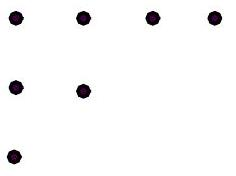
\includegraphics[max width=\textwidth, center]{2025_09_05_3ba26226ec0baddb5a03g-31}

Notemos que cambiando en este diagrama las filas por las columnas obtenemos otra partición de 7 , en este caso la partición $7=3+2+1+1$.\\
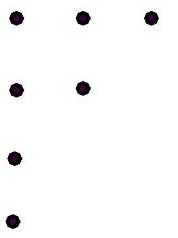
\includegraphics[max width=\textwidth, center]{2025_09_05_3ba26226ec0baddb5a03g-31(1)}

Función generatriz de $p(n)$. Una partición de $n$ queda determinada conociendo la cantidad de partes que son unos, la cantidad de partes que son dos, etc... Dicho de otra manera, la cantidad $p(n)$ de particiones de $n$ es igual a la cantidad de soluciones enteras no negativas $e_{1}, e_{2}, e_{3} \ldots$ de la ecuación $e_{1}+2 e_{2}+3 e_{3}+\cdots=n$, lo que es igual al coeficiente de $x^{n}$ del producto

$$
\left(1+x+x^{2}+x^{3}+\cdots\right)\left(1+x^{2}+x^{4}+x^{6}+\cdots\right)\left(1+x^{3}+x^{6}+x^{9}+\cdots\right) \cdots \cdots
$$

En otras palabras,

$$
\sum_{n=0}^{\infty} p(n) x^{n}=\frac{1}{1-x} \frac{1}{1-x^{2}} \frac{1}{1-x^{3}} \ldots \ldots .
$$

Luego, la función generatriz de $p(n)$ es $G(x)=\frac{1}{1-x} \frac{1}{1-x^{2}} \frac{1}{1-x^{3}} \ldots \ldots$.

Particiones con restricciones. Denotemos por $p(n, I)$ a la cantidad de particiones de $n$ que tienen todas sus partes impares y definamos $p(0, I)=1$. Por ejemplo, para $n=7$ las particiones que tienen todas sus partes impares son

$$
7, \quad 5+1+1, \quad 3+3+1, \quad 3+1+1+1+1, \quad 1+1+1+1+1+1+1
$$

es decir, $p(7, I)=5$. Análogamente, denotemos por $p(n, D)$ a la cantidad de particiones de $n$ que tienen todas sus partes distintas y definamos $p(0, D)=1$. Por ejemplo, para $n=7$ las particiones que tienen todas sus partes distintas son

$$
7, \quad 6+1, \quad 5+2, \quad 4+3, \quad 4+2+1
$$

es decir, $p(7, D)=5$.\\
Como vemos, $p(7, I)=p(7, D)$. El siguiente teorema muestra que esto no es casualidad.\\
Teorema: Para todo $n \in \mathbb{N}$ vale que $p(n, I)=p(n, D)$.\\
Demostración: Con un argumento análogo al usado para hallar la función generatriz de $p(n)$ se ve que la función generatriz de $p(n, I)$ es

$$
G(x)=\frac{1}{1-x} \frac{1}{1-x^{3}} \frac{1}{1-x^{5}} \cdots \cdots
$$

Luego,

$$
\begin{aligned}
& \sum_{n=0}^{\infty} p(n, I) x^{n}=\frac{1}{1-x} \frac{1}{1-x^{3}} \frac{1}{1-x^{5}} \ldots \ldots= \\
& =\frac{1-x^{2}}{(1-x)\left(1-x^{2}\right)} \frac{1-x^{4}}{\left(1-x^{3}\right)\left(1-x^{4}\right)} \frac{1-x^{6}}{\left(1-x^{5}\right)\left(1-x^{6}\right)} \ldots \ldots= \\
& =\frac{1-x^{2}}{1-x} \frac{1-x^{4}}{1-x^{2}} \frac{1-x^{6}}{1-x^{3}} \ldots \ldots=(1+x)\left(1+x^{2}\right)\left(1+x^{3}\right) \ldots \ldots
\end{aligned}
$$

El resultado sigue observando que el coeficiente de $x^{n}$ de $(1+x)\left(1+x^{2}\right)\left(1+x^{3}\right) \ldots \ldots$. es $p(n, D)$ -

Teorema: Para todo $n \in \mathbb{N}$ se verifica

$$
(1-x)\left(1-x^{2}\right)\left(1-x^{3}\right) \ldots \ldots=1+\sum_{n=1}^{\infty}\left[p\left(n, D^{+}\right)-p\left(n, D^{-}\right)\right] x^{n}
$$

donde $p\left(n, D^{+}\right)$denota la cantidad de particiones de $n$ que tienen un número par de partes, todas distintas y $p\left(n, D^{-}\right)$la cantidad de particiones de $n$ que tienen un número impar de partes, todas distintas.

Dejamos la demostración de este teorema como ejercicio.\\
Teorema: La cantidad de particiones de $n$ que tienen a lo sumo $k$ partes es igual a la cantidad de particiones de $n$ tales que ninguna parte supera a $k$.\\
Demostración: Si en un diagrama de Ferrers con a lo sumo $k$ filas cambiamos filas por columnas, obtenemos un diagrama de Ferrers que tiene a lo sumo $k$ puntos en cada fila. Recíprocamente, si en un diagrama de Ferrers que tiene a lo sumo $k$ puntos en cada fila cambiamos filas por columnas entocnes obtenemos un diagrama de Ferrers que tiene a lo sumo $k$ filas.\\
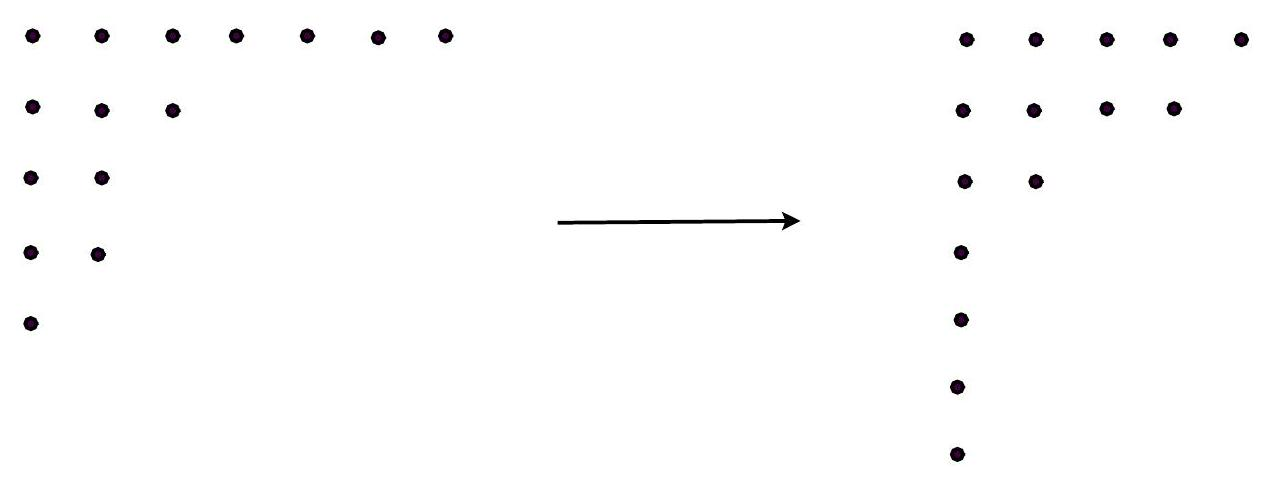
\includegraphics[max width=\textwidth, center]{2025_09_05_3ba26226ec0baddb5a03g-33}

Luego, basta notar que las particiones de $n$ en a lo sumo $k$ partes son aquellas cuyo diagrama de Ferrers tiene a lo sumo $k$ filas y que las particiones de $n$ tales que ninguna parte supera a $k$ son aquellas cuyo diagrama de Ferrers tiene a lo sumo $k$ puntos en cada fila.\\
Denotemos por $p(n, \leq k)$ a la cantidad de particiones de $n$ que tienen a lo sumo $k$ partes y definamos $p(0, \leq k)=1$. Observando que el coeficiente de $x^{n}$ de

$$
\left(1+x+x^{2}+\cdots\right)\left(1+x^{2}+x^{4}+\cdots\right) \ldots\left(1+x^{k}+x^{2 k}+\cdots\right)
$$

es la cantidad de particiones de $n$ tales que ninguna parte supera a $k$, por el teorema se tiene que

$$
\sum_{n=0}^{\infty} p(n, \leq k) x^{n}=\frac{1}{(1-x)\left(1-x^{2}\right) \ldots\left(1-x^{k}\right)}
$$

Teorema: Sea $k \in \mathbb{N}$. Entonces la función generatriz de $p(n, k)$ es

$$
G(x)=\frac{x^{k}}{(1-x)\left(1-x^{2}\right) \ldots\left(1-x^{k}\right)}
$$

es decir,

$$
\sum_{n=1}^{\infty} p(n, k) x^{n}=\frac{x^{k}}{(1-x)\left(1-x^{2}\right) \ldots\left(1-x^{k}\right)}
$$

Demostración: Recordemos que $p(n, k)$ es la cantidad de particiones de $n$ que tienen exactamente $k$ partes. Luego, $p(n, k)=p(n, \leq k)-p(n, \leq k-1)$ para todo $n \in \mathbb{N}$. Teniendo en cuenta, además, que $p(0, \leq k)=1=p(0, \leq k+1)$ se tiene entonces que

$$
\begin{aligned}
& \sum_{n=1}^{\infty} p(n, k) x^{n}=\sum_{n=1}^{\infty} p(n, \leq k) x^{n}-\sum_{n=1}^{\infty} p(n, \leq k-1) x^{n}= \\
& =\sum_{n=0}^{\infty} p(n, \leq k) x^{n}-\sum_{n=0}^{\infty} p(n, \leq k-1) x^{n}= \\
& =\frac{1}{(1-x)\left(1-x^{2}\right) \ldots\left(1-x^{k}\right)}-\frac{1}{(1-x)\left(1-x^{2}\right) \ldots\left(1-x^{k-1}\right)}= \\
& =\frac{1}{(1-x)\left(1-x^{2}\right) \ldots\left(1-x^{k-1}\right)}\left(\frac{1}{1-x^{k}}-1\right)= \\
& =\frac{x^{k}}{(1-x)\left(1-x^{2}\right) \ldots\left(1-x^{k}\right)}
\end{aligned}
$$

Una relación de recurrencia para $p(n)$. Si bien no se conoce ninguna fórmula explícita para calcular $p(n)$, veremos que hay una relación de recurrencia que nos permite calcularlo.

Lema: Para cada $k \in \mathbb{N}$ sean $\alpha_{k}=\frac{3 k^{2}-k}{2}$ y $\beta_{k}=\frac{3 k^{2}+k}{2}$. Entonces\\
$(1-x)\left(1-x^{2}\right)\left(1-x^{3}\right) \ldots=1+\sum_{k=1}^{\infty}(-1)^{k}\left(x^{\alpha_{k}}+x^{\beta_{k}}\right)=1-\left(x+x^{2}\right)+\left(x^{5}+x^{7}\right)-\left(x^{12}+x^{15}\right)-\cdots$

Demostración: Recordemos que

$$
(1-x)\left(1-x^{2}\right)\left(1-x^{3}\right) \ldots \ldots=1+\sum_{n=1}^{\infty}\left[p\left(n, D^{+}\right)-p\left(n, D^{-}\right)\right] x^{n}
$$

donde $p\left(n, D^{+}\right)$denota la cantidad de particiones de $n$ que tienen un número par de partes, todas distintas y $p\left(n, D^{-}\right)$la cantidad de particiones de $n$ que tienen un número impar de partes, todas distintas. Luego, basta ver que $p\left(n, D^{+}\right)-p\left(n, D^{-}\right)=0$ para todo $n$ salvo cuando $n=\alpha_{k}$ o $\beta_{k}(k=1,2, \ldots)$, en cuyo caso vale $(-1)^{k}$.

Para ello, consideremos el diagrama de Ferrers de una partición de $n$ que tenga todas sus partes distintas. Sea $k$ tal que la fila $i$ tiene exactamente un punto más que la fila $i+1$ para todo $i$ entre $1 \mathrm{y} k-1 \mathrm{y}$ la fila $k$ es la última fila o tiene al menos 2 puntos más que la fila $k+1$ y sea $b$ la cantidad de puntos que tiene la última fila.\\
Por ejemplo, en el diagrama\\
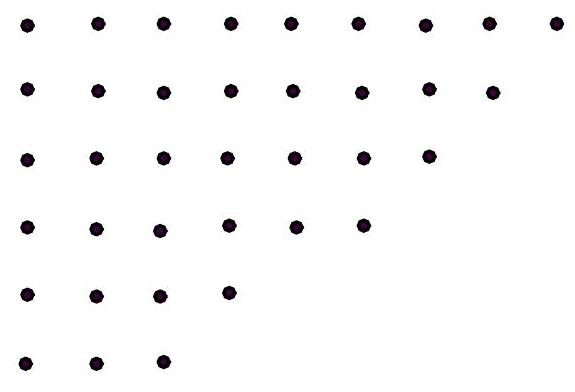
\includegraphics[max width=\textwidth, center]{2025_09_05_3ba26226ec0baddb5a03g-35}\\
$k=4$ pues la fila 1 tiene un punto más que la fila 2 , la fila 2 tiene un punto más que la fila 3, la fila 3 tiene un punto más que la fila 4 y la fila 4 tiene dos puntos más que la fila 5 y $b=3$ pues la última fila tiene tres puntos y en el diagrama\\
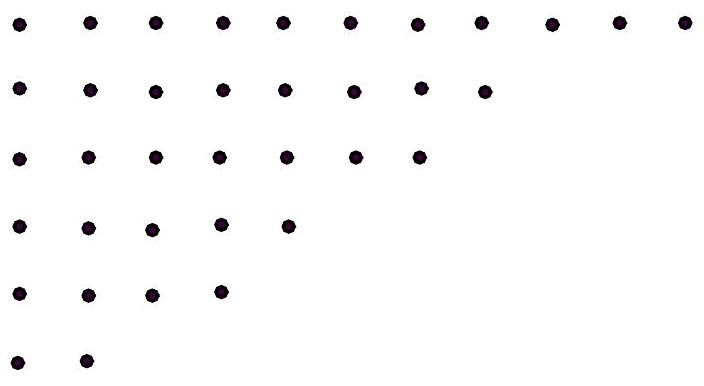
\includegraphics[max width=\textwidth, center]{2025_09_05_3ba26226ec0baddb5a03g-35(2)}\\
$k=1$ y $b=2$.\\
Si tenemos un diagrama que representa una partición de $n$ que tiene todas sus partes distintas para el cual $k<b$ y movemos el último punto de cada una de las primeras $k$ filas debajo de la última fila formando una nueva fila de $k$ puntos obtenemos una partición de $n$ que tiene todas sus partes distintas y una fila más, salvo en el caso en que $b=k+1$ y haya exactamente $k$ filas. Llamemos transformación $A$ a esta aplicación.\\
Por ejemplo,\\
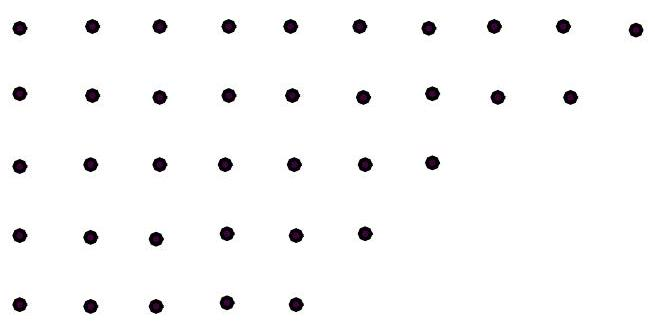
\includegraphics[max width=\textwidth, center]{2025_09_05_3ba26226ec0baddb5a03g-35(1)}\\
muestra un diagrama de Ferrers de una partición de 37 que tiene todas sus partes distintas. En este caso $k=2$ y $b=5$.\\
Si en este diagrama movemos el último punto de cada una de las primeras 2 filas debajo de la última fila formando una nueva fila de 2 puntos obtenemos una partición de 37 con todas sus partes distintas y una fila más.\\
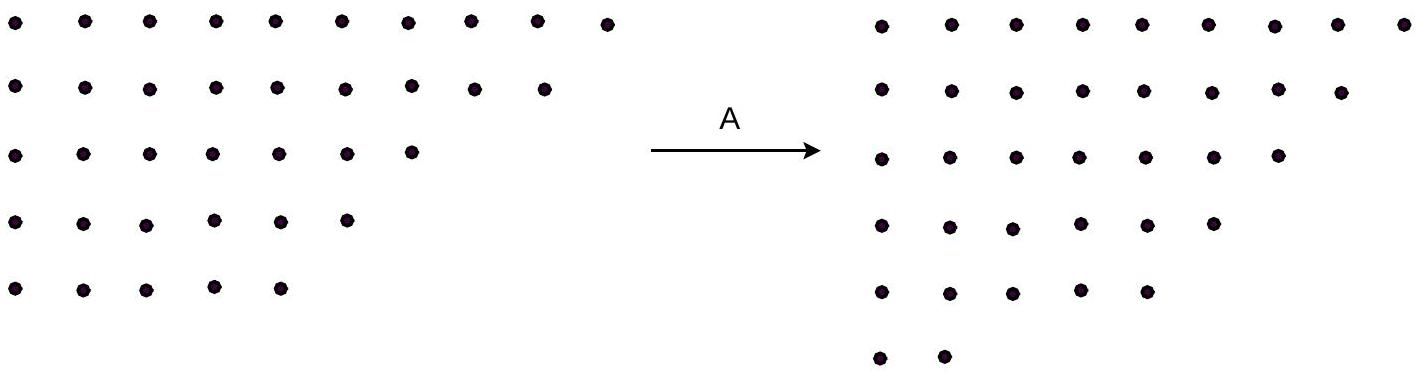
\includegraphics[max width=\textwidth, center]{2025_09_05_3ba26226ec0baddb5a03g-36(1)}

Notemos que si aplicáramos esta transformación en el caso en que $b=k+1$ y hay exactamente $k$ filas\\
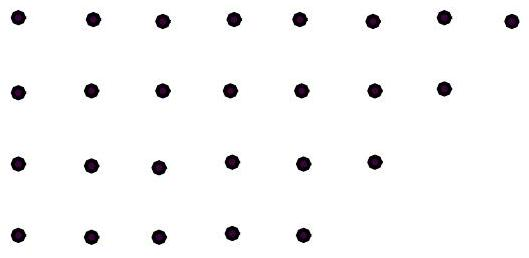
\includegraphics[max width=\textwidth, center]{2025_09_05_3ba26226ec0baddb5a03g-36(2)}\\
no obtendríamos una partición de $n$ en partes distintas. Observemos que este caso ocurre si y sólo si hay $k$ filas, la última fila tiene $k+1$ puntos y cada fila tiene exactamente un punto menos que la fila anterior, lo que pasa si y sólo si

$$
n=(k+1)+(k+2)+\cdots+(k+k)=k^{2}+\frac{k(k+1)}{2}=\frac{3 k^{2}+k}{2}
$$

es decir, si y sólo si $n=\beta_{k}$\\
Si, en cambio, tenemos un diagrama que representa una partición de $n$ que tiene todas sus partes distintas para el cual $k \geq b$ y movemos cada uno de los $b$ puntos de la última fila al final de cada una de las primeras $b$ filas obtenemos una partición de $n$ que tiene todas sus partes distintas y una fila menos, salvo en el caso en que $b=k$ y haya exactamente $k$ filas. Llamemos transformación $B$ a esta aplicación.\\
Por ejemplo, si tenemos el diagrama\\
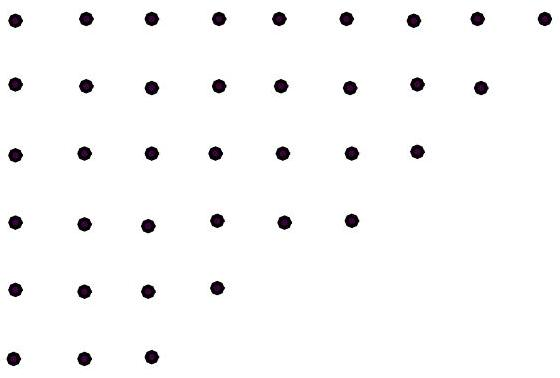
\includegraphics[max width=\textwidth, center]{2025_09_05_3ba26226ec0baddb5a03g-36}\\
que representa una partición de 37 que tiene todas sus partes distintas donde $k=4$ y $b=3$, y colocamos cada uno de los 3 puntos que componen la última fila al final de cada una de\\
las primeras 3 filas obtenemos una partición de 37 que tiene todas sus partes distintas y una fila menos.\\
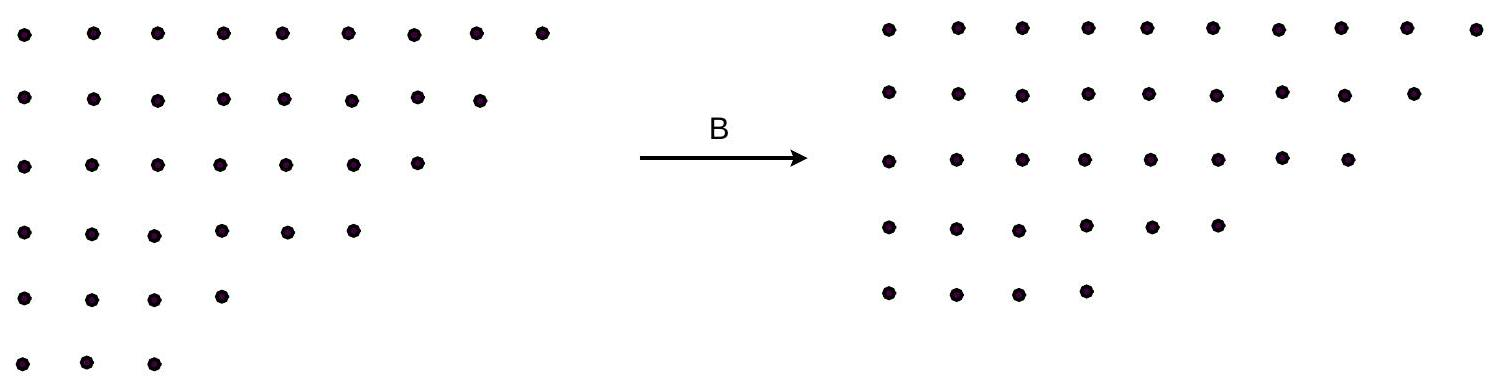
\includegraphics[max width=\textwidth, center]{2025_09_05_3ba26226ec0baddb5a03g-37(1)}

Notemos que si aplicáramos esta transformación en el caso en que hay exactamente $k$ filas y $b=k$\\
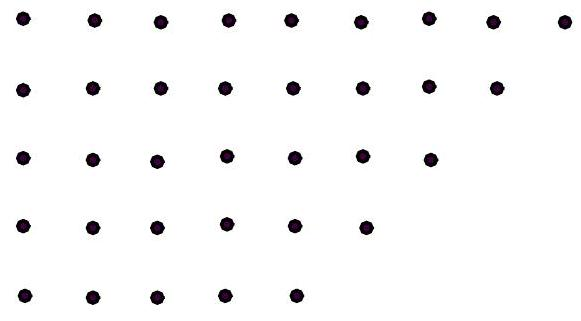
\includegraphics[max width=\textwidth, center]{2025_09_05_3ba26226ec0baddb5a03g-37}\\
no obtendríamos un diagrama con una fila menos. Observemos que este caso ocurre si y sólo si hay $k$ filas, la última fila tiene $k$ puntos y cada fila tiene exactamente un punto menos que la fila anterior, lo que pasa si y sólo si

$$
n=k+(k+1)+(k+2)+\cdots+(k+k-1)=k^{2}+\frac{(k-1) k}{2}=\frac{3 k^{2}-k}{2}
$$

es decir, si y sólo si $n=\alpha_{k}$\\
Luego, si $n \neq \alpha_{k}, \beta_{k}$ para todo $k$, podemos definir una aplicación $f$ del conjunto de diagramas de Ferrers con $n$ puntos que tienen un número par de filas en el conjunto de diagramas de Ferrers con $n$ puntos que tienen un número impar de filas de la siguiente manera:\\
Dado un diagrama de Ferrers $\mathcal{F}$ con $n$ puntos que tiene un número par de filas definimos $f(\mathcal{F})$ como el diagrama que resulta de aplicarle la transformación $A$ a $\mathcal{F}$ si en $\mathcal{F}$ se tiene que $k<b$ o como el diagrama que resulta de aplicarle la transformación $B$ a $\mathcal{F}$ si en $\mathcal{F}$ se tiene que $k \geq b$.\\
Dejamos como ejercicio mostrar que esta aplicación es biyectiva.\\
Ahora, observando que hay tantos diagramas de Ferrers con $n$ puntos que tienen un número par de filas como particiones de $n$ en un número par de partes, todas distintas, y que lo mismo vale si cambiamos "par" por "impar", entonces de lo anteriror resulta que, si $n \neq \alpha_{k}, \beta_{k}$ para todo $k$, entonces $p\left(n, D^{+}\right)=p\left(n, D^{-}\right)$, es decir, $p\left(n, D^{+}\right)-p\left(n, D^{-}\right)=0$.

Veamos ahora qué ocurre en el caso en que $n=\alpha_{k}$ o $n=\beta_{k}$.\\
Notemos que si $n=\alpha_{k}$, entonces hay un único diagrama de Ferrers al que no le podemos aplicar la transformación $B$ : el que tiene exactamente $k$ filas y para el cual vale $b=k$. Este diagrama, al que denotaremos por $\mathcal{F}_{0}$ tiene una cantidad par de filas si y sólo si $k$ es par. Además, no existe ninguno al que no le podamos aplicar la transformación $A$. Luego, si $k$ es par ahora podemos definir $f$ en la misma forma que antes, pero del conjunto de diagramas de Ferrers con $n$ puntos que tienen un número par de filas y son distintos de $\mathcal{F}_{0}$ en el conjunto de diagramas de Ferrers con $n$ puntos que tienen un número impar de filas. Esta aplicación es biyectiva y por lo tanto en este caso se tiene que $p\left(n, D^{+}\right)-1=p\left(n, D^{-}\right)$, es decir, $p\left(n, D^{+}\right)-p\left(n, D^{-}\right)=1=(-1)^{k}$.\\
Análogamente, si $k$ es impar podemos definir $f$ en la misma forma que antes, pero del conjunto de diagramas de Ferrers con $n$ puntos que tienen un número par de filas en el conjunto de diagramas de Ferrers con $n$ puntos que tienen un número impar de filas y son distintos de $\mathcal{F}_{0}$. Esta aplicación es biyectiva y por lo tanto en este caso se tiene que $p\left(n, D^{+}\right)=p\left(n, D^{-}\right)-1$, es decir, $p\left(n, D^{+}\right)-p\left(n, D^{-}\right)=-1=(-1)^{k}$.\\
Finalmente, si $n=\beta_{k}$ entonces hay un único diagrama de Ferrers al que no le podemos aplicar la transformación $A$ : el que tiene exactamente $k$ filas y para el cual vale $b=k+1$. Este diagrama tiene una cantidad par de filas si y sólo si $k$ es par. Además, no existe ninguno al que no le podamos aplicar la transformación $B$. Luego, razonando como en el caso anterior resulta que $p\left(n, D^{+}\right)-p\left(n, D^{-}\right)=(-1)^{k}$, tanto para $k$ par como para $k$ impar. ㅁ

Veamos ahora cómo este lema nos permite hallar una relación de recurrencia para $p(n)$. Sabemos que

$$
\sum_{n=0}^{\infty} p(n) x^{n}=\frac{1}{1-x} \frac{1}{1-x^{2}} \frac{1}{1-x^{3}} \ldots \ldots
$$

Luego,

$$
\left((1-x)\left(1-x^{2}\right)\left(1-x^{3}\right) \ldots\right) \sum_{n=0}^{\infty} p(n) x^{n}=1
$$

Ahora, usando el lema, se tiene que

$$
\left(1+\sum_{k=1}^{\infty}(-1)^{k}\left(x^{\alpha_{k}}+x^{\beta_{k}}\right)\right)\left(\sum_{n=0}^{\infty} p(n) x^{n}\right)=1
$$

donde $\alpha_{k}=\frac{3 k^{2}-k}{2}$ y $\beta_{k}=\frac{3 k^{2}+k}{2}$, es decir,

$$
\left(1-x-x^{2}+x^{5}+x^{7}-x^{12}-x^{15}+\cdots\right)\left(p(0)+p(1) x+p(2) x^{2}+p(3) x^{3}+\cdots\right)=1
$$

ya que $p(0)=1$. Por lo tanto, el coeficiente de $x^{n}$ en el miembro izquierdo de esta igualdad debe ser cero para todo $n \geq 1$. Luego, definiendo $p(m)=0$ para todo $m<0$, resulta que

$$
p(n)-p(n-1)-p(n-2)+p(n-5)+p(n-7)-p(n-12)-p(n-15)+\cdots=0
$$

de donde

$$
\begin{aligned}
& p(n)=p(n-1)+p(n-2)-p(n-5)-p(n-7)+p(n-12)+p(n-15)-\cdots= \\
& \quad=p\left(n-\alpha_{1}\right)+p\left(n-\beta_{1}\right)-p\left(n-\alpha_{2}\right)-p\left(n-\beta_{2}\right)+p\left(n-\alpha_{3}\right)+p\left(n-\beta_{3}\right)-\cdots
\end{aligned}
$$

es decir,

$$
p(n)=\sum_{k=1}^{\infty}(-1)^{k+1}\left[p\left(n-\alpha_{k}\right)+p\left(n-\beta_{k}\right)\right]
$$

Notemos que la suma de la derecha es, en realidad, una suma finita.\\
Por ejemplo, usando esta recurrencia y el hecho de que $p(0)=1$, vemos que los valores de $p(n)$ para $n$ entre 1 y 8 son $p(1)=p(0)=1, p(2)=p(1)+p(0)=2, p(3)=p(2)+p(1)=3$, $p(4)=p(3)+p(2)=5, p(5)=p(4)+p(3)-p(0)=7, p(6)=p(5)+p(4)-p(1)=11$, $p(7)=p(6)+p(5)-p(2)-p(0)=15$ у $p(8)=p(7)+p(6)-p(3)-p(1)=22$ 。

\section*{10. Particiones de un conjunto.}
Recordemos que ya hemos visto dos problemas relacionados con las particiones de un conjunto. El primero consistía en hallar la cantidad de particiones de un conjunto de $n$ elementos en $k$ partes. A estos números, a los que denotamos por $S(n, k)$, los llamamos números de Stirling de segunda especie. El segundo problema consistía en determinar la cantidad total de particiones de un conjunto de $n$ elementos. A estos números, a los que denotamos por $B_{n}$, los llamamos números de Bell.\\
En esta sección consideraremos ahora otro problema relacionado con las particiones de un conjunto $\Omega$ de $n$ elementos.\\
Dados $n$ enteros no negativos $\lambda_{1}, \lambda_{2}, \ldots, \lambda_{n}$ tales que $n=1 \lambda_{1}+2 \lambda_{2}+\cdots+n \lambda_{n}$, queremos determinar cuántas particiones hay de $\Omega$ que tengan $\lambda_{1}$ partes con un solo elemento, $\lambda_{2}$ partes con 2 elementos, $\ldots, \lambda_{n}$ partes con $n$ elementos.\\
Para concretar la idea consideremos el siguiente ejemplo. Sea $\Omega$ un conjunto de $n=15$ elementos y sean $\lambda_{1}=1, \lambda_{2}=4, \lambda_{3}=2$ y $\lambda_{i}=0$ para $4 \leq i \leq 15$. ¿Cuántas particiones hay de $\Omega$ que tengan 1 parte con un elemento, 4 partes con dos elementos y 2 partes con tres elementos? Notemos que podemos pensar este problema de la siguiente manera:\\
Supongamos que queremos particionar un conjunto de 15 diplomáticos en 7 partes, una con un diplomático, cuatro con 2 diplomáticos y dos con 3 diplomáticos. ¿De cuántas maneras lo podemos hacer? Llamemos $x$ a este número y ahora calculemos $x$ resolviendo el siguiente problema de dos maneras distintas:\\
Dado un conjunto con 15 diplomáticos, queremos seleccionar uno para enviar a Austria, dos para enviar a Brasil, dos para Colombia, dos para Dinamarca, dos para EEUU, tres para Finlandia y tres para Grecia. ¿De cuántas maneras podemos hacer esto?\\
Notando que esto es lo mismo que determinar la cantidad de permutaciones con repetición de ABBCCDDEEFFFGGG, resulta que la solución es $\frac{15!}{(1!)^{1}(2!)^{4}(3!)^{2}}$. Ahora resolvamos este problema de la siguiente manera:

Primero particionamos el conjunto de los 15 diplomáticos en en 7 partes, una con un diplomático, cuatro con 2 diplomáticos y dos de 3 diplomáticos y luego asignamos los diplomáticos de cada parte con $k$ elementos a los países a los que hay que enviar $k$ diplomáticos. La solución entonces es $x 1!4!2!$. Luego debe ser $\frac{15!}{(1!)^{1}(2!)^{4}(3!)^{2}}=x 1!4!2!$, de donde obtenemos que $x=\frac{15!}{(1!)^{1}(2!)^{4}(3!)^{2} 1!4!2!}$.\\
Generalizando esta idea se tiene que si $\lambda_{1}, \lambda_{2}, \ldots, \lambda_{n}$ son enteros no negativos tales que $n=1 \lambda_{1}+2 \lambda_{2}+\cdots+n \lambda_{n}$ entonces la cantidad de particiones de un conjunto de $n$ elementos que tienen $\lambda_{1}$ partes con un solo elemento, $\lambda_{2}$ partes con 2 elementos, $\ldots, \lambda_{n}$ partes con $n$ elementos es

$$
\frac{n!}{(1!)^{\lambda_{1}}(2!)^{\lambda_{2}} \ldots(n!)^{\lambda_{n}} \lambda_{1}!\lambda_{2}!\ldots \lambda_{n}!}
$$

Configuración cíclica. Sea $\pi \in S_{9}$ la permutación $\pi=(2)$ (6) (5 7) (8 9) (14 3). Esta permutación tiene dos ciclos de longitud 1, dos ciclos de longitud 2 y un ciclo de longitud 3. ¿Cuántas permutaciones de $S_{9}$ tienen la misma configuración cíclica que $\pi$, es decir, tienen dos ciclos de longitud 1 , dos ciclos de longitud 2 y un ciclo de longitud 3 ?\\
Para resolver este problema primero determinemos cuántas particiones hay del conjunto de $n=9$ elementos $\Omega=\{1,2, \ldots, 9\}$, que tengan $\lambda_{1}=2$ partes con un elemento, $\lambda_{2}=2$ partes con dos elementos y $\lambda_{3}=1$ partes con tres elementos. Tomando $\lambda_{i}=0$ para $i=4,5, \ldots, 9$ resulta que lo que queremos es determinar cuántas particiones hay de $\Omega$ que tengan $\lambda_{1}$ partes con un solo elemento, $\lambda_{2}$ partes con 2 elementos, $\ldots, \lambda_{n}$ partes con $n$ elementos, donde $\lambda_{1}, \ldots, \lambda_{n}$ satisfacen $n=1 \lambda_{1}+2 \lambda_{2}+\cdots+n \lambda_{n}$. Luego, la cantidad de particiones es

$$
\frac{9!}{(1!)^{2}(2!)^{2}(3!)^{1} 2!2!1!}
$$

Ahora notemos que cada parte con $k$ elementos da lugar a $(k-1)$ ! ciclos distintos de longitud $k$. Luego, la respuesta a nuestro problema es

$$
\frac{9!}{(1!)^{2}(2!)^{2}(3!)^{1} 2!2!1!} 0!0!1!1!2!=\frac{9!}{(1!)^{2}(2!)^{2}(3!)^{1} 2!2!1!}(0!)^{2}(1!)^{2}(2!)^{1}
$$

En general, dados $\lambda_{1}, \lambda_{2}, \ldots, \lambda_{n}$, queremos determinar cuántas permutaciones de $S_{n}$ tienen $\lambda_{1}$ ciclos de longitud $1, \lambda_{2}$ ciclos de longitud $2, \ldots, \lambda_{n}$ ciclos de longitud $n$. Notemos que si $n \neq 1 \lambda_{1}+2 \lambda_{2}+\cdots+n \lambda_{n}$ entonces no puede existir ninguna permutación en $S_{n}$ con esa configuración cíclica, por lo tanto podemos suponer que $n=1 \lambda_{1}+2 \lambda_{2}+\cdots+n \lambda_{n}$ y en tal caso el problema se resuelve determinando primero cuántas particiones hay de $\{1,2, \ldots, n\}$ que tengan $\lambda_{1}$ partes con un solo elemento, $\lambda_{2}$ partes con 2 elementos, $\ldots, \lambda_{n}$ partes con $n$ elementos y luego multiplicando este resultado por la cantidad de permutaciones cíclicas de cada una de esas partes. Luego, la respuesta es

$$
\begin{aligned}
& \frac{n!}{(1!)^{\lambda_{1}}(2!)^{\lambda_{2}} \ldots(n!)^{\lambda_{n}} \lambda_{1}!\lambda_{2}!\ldots \lambda_{n}!}(0!)^{\lambda_{1}}(1!)^{\lambda_{2}} \ldots((n-1)!)^{\lambda_{n}}= \\
& =\frac{n!}{1^{\lambda_{1}} 2^{\lambda_{2}} \ldots n^{\lambda_{n}} \lambda_{1}!\lambda_{2}!\ldots \lambda_{n}!}
\end{aligned}
$$

Notación: Denotaremos por $C\left(\lambda_{1}, \lambda_{2}, \ldots, \lambda_{n}\right)$ a la cantidad de permutaciones de $S_{n}$ que tienen $\lambda_{1}$ ciclos de longitud $1, \lambda_{2}$ ciclos de longitud $2, \ldots, \lambda_{n}$ ciclos de longitud $n$.

Ejemplo: Permutaciones de $S_{4}$.\\
Agrupemos las 24 permutaciones de $S_{4}$ según su configuración cíclica:\\
Con la configuración $\lambda_{1}=0, \lambda_{2}=0, \lambda_{3}=0, \lambda_{4}=1$, se tienen las $C(0,0,0,1)=\frac{4!}{4^{1} 1!}=6$ permutaciones (123 4), (1423), (1342), (1243), (1324) y (1432).\\
Con la configuración $\lambda_{1}=1, \lambda_{2}=0, \lambda_{3}=1, \lambda_{4}=0$, las $C(1,0,1,0)=\frac{4!}{1^{1} 3^{1} 1!1!}=8$ permutaciones (1) (2 34 ), (1) (2 43 3), (2) (1 34 ), (2) (1 43 ), (3) (1 2 4), (3) (1 42 ), (4) ( 123 ) y (4) ( 132 ).

Con la configuración $\lambda_{1}=0, \lambda_{2}=2, \lambda_{3}=0, \lambda_{4}=0$, las $C(0,2,0,0)=\frac{4!}{2^{2} 2!}=3$ permutaciones $(12)$ ( 34 ), ( 13 ) ( 24 ) y ( 14 ) ( 23 ).\\
Con la configuración $\lambda_{1}=2, \lambda_{2}=1, \lambda_{3}=0, \lambda_{4}=0$, las $C(2,1,0,0)=\frac{4!}{1^{2} 2^{1} 2!1!}=6$ permutaciones (1) (2) (3 4), (1) (3) (2 4), (1) (4) (2 3), (2) (3) (1 4), (2) (4) (1 3) y (3) (4) (1 2). Con la configuración $\lambda_{1}=4, \lambda_{2}=0, \lambda_{3}=0, \lambda_{4}=0$, la $C(4,0,0,0)=\frac{4!}{1^{4} 4!}=1$ permutación (1) (2) (3) (4).

Indicador de ciclos. Definimos la función generatriz de $C\left(\lambda_{1}, \lambda_{2}, \ldots, \lambda_{n}\right)$ como el polinomio en las $n$ indeterminadas $t_{1}, t_{2}, \ldots, t_{n}$

$$
Z_{S_{n}}\left(t_{1}, t_{2}, \ldots, t_{n}\right)=\sum_{1 \lambda_{1}+2 \lambda_{2}+\cdots+n \lambda_{n}=n} C\left(\lambda_{1}, \lambda_{2}, \ldots, \lambda_{n}\right) t_{1}^{\lambda_{1}} t_{2}^{\lambda_{2}} \ldots t_{n}^{\lambda_{n}}
$$

$Z_{S_{n}}$ se llama el indicador de ciclos de $S_{n}$ pues cada uno de sus términos identifica una configuración y su coeficiente es la cantidad de permutaciones de $S_{n}$ que tienen dicha configuración. Por ejemplo, para $n=4$,

$$
Z_{S_{4}}=t_{1}{ }^{4}+6 t_{1}{ }^{2} t_{2}+3 t_{2}{ }^{2}+8 t_{1} t_{3}+6 t_{4}{ }^{4}
$$

\section*{11. Teoría de Polya.}
Comenzaremos por dar algunas nociones elementales sobre teoría de grupos que necesitaremos más adelante.

\section*{Grupos finitos.}
Definición: Sea $G$ un conjunto y sea * una operación en $G$, es decir, una función que a cada par de elementos $f, g \in G$ le asigna un elemento de $G$ al que denotamos por $f * g$. Diremos que ( $G, *$ ) es un grupo si se verifican\\
i) $*$ es asociativa, es decir, $f *(g * h)=(f * g) * h \quad \forall f, g, h \in G$\\
ii) * tiene elemento neutro, es decir, existe $e \in G$ tal que $f * e=f=e * f \forall f \in G$\\
iii) todo elemento de $G$ tiene inverso, es decir, para todo $f \in G$ existe un elemento de $G$ al que denotamos por $f^{-1}$ que satisface $f * f^{-1}=e=f^{-1} * f$

Diremos que ( $G, *$ ) es un grupo finito si es un grupo y, además, el conjunto $G$ es finito. Sea $(G, *)$ un grupo. Dejamos como ejercicio verificar que el elemento neutro y el inverso de cada elemento de $G$ son únicos.

Definición: Diremos que $H$ es un subgrupo de $G$ si $H \subseteq G$ y se verifican\\
i) $f * g \in H \quad \forall f, g \in H$\\
ii) $e \in H$ (donde $e$ es el elemento neutro de $G$ )\\
iii) $f^{-1} \in H \forall f \in H$ (donde $f^{-1}$ es el inverso de $f$ en $G$ )

Dejamos como ejercicio probar que si $H$ es un subgrupo de $G$ entonces $(H, *)$ es un grupo. Si $S$ es un subconjunto no vacío de $G$ entonces

$$
H=\left\{h_{1} * h_{2} * \ldots * h_{n} / n \in \mathbb{N} \text { y } h_{i} \in S \text { o } h_{i}^{-1} \in S(1 \leq i \leq n)\right\}
$$

es un subgrupo de $G$. Este subgrupo se llama el subgrupo generado por $S$ o también el subgrupo generado por $f_{1}, f_{2}, \ldots, f_{s}$, donde $f_{1}, f_{2}, \ldots, f_{s}$ son los elementos de $S$.

Ejemplo 1: El grupo simétrico.\\
Si se toma como operación la composición de funciones, el conjunto

$$
S_{n}=\{\pi:\{1,2, \ldots, n\} \longrightarrow\{1,2, \ldots, n\} / \pi \text { es biyectiva }\}
$$

es un grupo finito, llamado el grupo simétrico.\\
Indicador de ciclos de un subgrupo de $S_{n}$. Extenderemos ahora la definición del indicador de ciclos, que hemos definido para el grupo $S_{n}$, a los subgrupos de $S_{n}$. Si $H$ es un subgrupo de $S_{n}$, denotaremos por $C_{H}\left(\lambda_{1}, \lambda_{2}, \ldots, \lambda_{n}\right)$ a la cantidad de permutaciones de $H$ que tienen $\lambda_{1}$ ciclos de longitud $1, \lambda_{2}$ ciclos de longitud $2, \ldots, \lambda_{n}$ ciclos de longitud $n$, donde $\lambda_{1}, \ldots, \lambda_{n}$ satisfacen $1 \lambda_{1}+2 \lambda_{2}+\cdots+n \lambda_{n}=n$, y definimos el indicador de ciclos de $H$ como el polinomio en las $n$ indeterminadas $t_{1}, t_{2}, \ldots, t_{n}$

$$
Z_{H}\left(t_{1}, t_{2}, \ldots, t_{n}\right)=\sum_{1 \lambda_{1}+2 \lambda_{2}+\cdots+n \lambda_{n}=n} C_{H}\left(\lambda_{1}, \lambda_{2}, \ldots, \lambda_{n}\right) t_{1}^{\lambda_{1}} t_{2}^{\lambda_{2}} \ldots t_{n}^{\lambda_{n}}
$$

Por ejemplo, $H=\left\{\left(\begin{array}{lll}1 & 2 & 3 \\ 4\end{array}\right),\left(\begin{array}{lll}1 & 3\end{array}\right)\left(\begin{array}{lll}2 & 4\end{array}\right),\left(\begin{array}{llll}1 & 4 & 3 & 2\end{array}\right),(1)(2)(3)(4)\right\}$ es un subgrupo de $S_{4}$. En este caso $C_{H}\left(\lambda_{1}, \ldots \lambda_{4}\right)=0$ salvo en los casos $\lambda_{1}=0, \lambda_{2}=2, \lambda_{3}=0, \lambda_{4}=0 \mathrm{y} \lambda_{1}=0, \lambda_{2}=0, \lambda_{3}=0, \lambda_{4}=1$ y $\lambda_{1}=4, \lambda_{2}=0, \lambda_{3}=0, \lambda_{4}=0$. En el primer caso se tiene que $C_{H}(0,2,0,0)=1$, en el segundo que $C_{H}(0,0,0,1)=2$ y en el tercero que $C_{H}(4,0,0,0)=1$. Luego, el indicador de ciclos de $H$ es $Z_{H}=t_{2}{ }^{2}+2 t_{4}+t_{1}{ }^{4}$.

Observación: Dada $\pi \in S_{n}$, denotemos por $\lambda_{j}(\pi)$ a la cantidad de ciclos de $\pi$ de longitud $j(1 \leq j \leq n)$. Entonces, para cualquier subgrupo $H$ de $S_{n}$,

$$
Z_{H}\left(t_{1}, t_{2}, \ldots, t_{n}\right)=\sum_{\pi \in H} t_{1}^{\lambda_{1}(\pi)} t_{2}^{\lambda_{2}(\pi)} \ldots t_{n}^{\lambda_{n}(\pi)}
$$

Ejemplo 2: Grupo de rotaciones del octaedro.\\
Llamaremos cuerpo rígido a un sistema finito de puntos de $\mathbb{R}^{3}$ tal que la distancia entre dos cualesquiera de ellos se mantiene constante a través de un movimiento. Estamos interesados en aquellos movimientos del cuerpo rígido en el espacio cuya posición final se superpone con la posición inicial. A tales rotaciones las llamaremos rotaciones de simetría. Notemos que la composición de dos rotaciones de simetría es una rotación de simetría. Más aún, el conjunto de todas las rotaciones de simetría de un cuerpo rígido es un grupo con la composición. Si un punto queda fijo con el movimiento, tal movimiento es equivalente a una rotación alrededor de un eje que pasa por el punto fijo (Teorema de Euler). Por ejemplo, tomemos como cuerpo rígido el octaedro\\
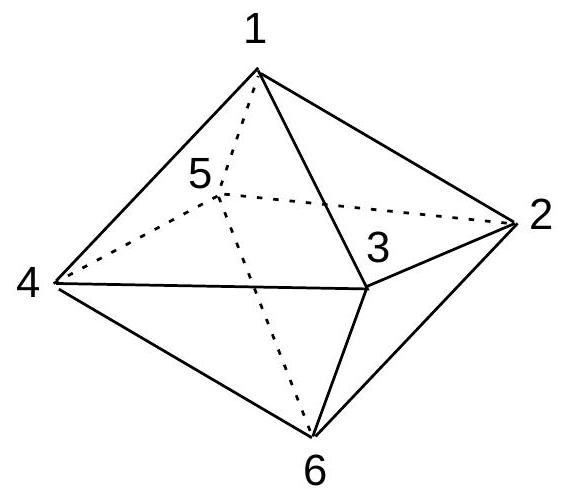
\includegraphics[max width=\textwidth, center]{2025_09_05_3ba26226ec0baddb5a03g-43}\\
donde hemos fijado una numeración de sus vértices, y consideremos las siguientes rotaciones\\
$R_{1}=$ giro de $90^{0}$ alrededor del eje 16 que lleva el vértice 5 a 2\\
$R_{2}$ = giro de $180^{0}$ alrededor del eje 16 que lleva el vértice 5 a 3\\
$R_{3}=$ giro de $270^{0}$ alrededor del eje 16 que lleva el vértice 5 a 4\\
$R_{4}=$ giro de $360^{0}$ alrededor del eje $16=$ identidad\\
Observemos además que estas son las únicas rotaciones de simetría del octaedro que dejan fijo el vértice 1 . Más aún, notemos que $R_{1}, R_{2}, R_{3}$ y $R_{4}$ dejan fijos los vértices 1 y 6 y que $R_{1}$ lleva el vértice 5 a 2 , el vértice 2 a 3,3 a 4 y 4 a $5, R_{2}$ lleva 5 a 3,3 a 5,2 a 4 y 4 a 2 , $R_{3}$ lleva 5 a 4,4 a 3,3 a 2 y 2 a 5 . Luego, $R_{1}, R_{2}, R_{3}$ y $R_{4}$ son cuatro rotaciones distintas y son las únicas que dejan fijo al vértice 1 .\\
Dejamos como ejercicio comprobar que el conjunto $\left\{R_{1}, R_{2}, R_{3}, R_{4}\right\}$ es un grupo con la composición. Por ejemplo, el inverso de $R_{1}$ es $R_{3}$ ya que la composición de $R_{1}$ con $R_{3}$ es la identidad. Sin embargo, este grupo no contiene todas las rotaciones de simetría del octaedro. Por ejemplo, una rotación de $90^{\circ}$ alrededor del eje 53 no fija al vértice 1 , por lo tanto no puede ser ninguna de las anteriores.\\
Si agregamos las 5 rotaciones $T_{1}, T_{2}, \ldots T_{5}$ que llevan el vértice 1 a cada uno de los otros vértices (y por lo tanto son todas distintas), que son $T_{1}=$ giro de $90^{\circ}$ alrededor del eje 53 que lleva 1 a 2\\
$T_{2}=$ giro de $90^{\circ}$ alrededor del eje 42 que lleva 1 a 3\\
$T_{3}=$ giro de $270^{0}$ alrededor del eje 53 que lleva 1 a 4\\
$T_{4}=$ giro de $270^{0}$ alrededor del eje 42 que lleva 1 a 5\\
$T_{5}=$ giro de $180^{0}$ alrededor del eje 42 que lleva 1 a 6\\
obtenemos, por composición con las anteriores, las siguientes rotaciones de simetría del octaedro: $T_{k} R_{i}(1 \leq k \leq 5,1 \leq i \leq 4)$.\\
Veamos que son todas distintas. Supongamos que $T_{p} R_{q}=T_{u} R_{v}$. Como $R_{q}$ y $R_{v}$ dejan fijo al vértice 1 , se tiene que $T_{p} R_{q}(1)=T_{u} R_{v}(1) \Longrightarrow T_{p}(1)=T_{v}(1)$, de donde debe ser $p=u$. Luego, $T_{p} R_{q}=T_{p} R_{v}$, y por lo tanto $T_{p}{ }^{-1} T_{p} R_{q}=T_{p}{ }^{-1} T_{p} R_{v}$, con lo cual $R_{q}=R_{v}$ lo cual ocurre si y sólo si $q=v$.\\
Además, dado que $R_{i}$ fija el vértice 1 para todo i y ninguna de las $T_{k}$ fija el 1 , se tiene que $T_{k} R_{j} \neq R_{i} \forall 1 \leq i, j \leq 4,1 \leq k \leq 5$.\\
Luego, el conjunto

$$
G=\left\{R_{i} / 1 \leq i \leq 4\right\} \cup\left\{T_{k} R_{i} / 1 \leq k \leq 5,1 \leq i \leq 4\right\}
$$

tiene 24 elementos, y todos ellos son rotaciones de simetría del octaedro.\\
Veamos ahora que $G$ es el grupo formado por todas las rotaciones de simetría del octaedro, es decir, que toda rotación de simetría del octaedro es alguno de los 24 elementos de $G$.\\
Sea $W$ una rotación de simetría del octaedro. Si $W(1)=1$, entonces $W=R_{i}$ para algún $i$ entre 1 y 4 y por lo tanto $W \in G$. Y si $W(1)=m$, donde m es alguno de los vértices $2,3,4,5$ o 6 , sea $k(1 \leq k \leq 5)$ tal que $T_{k}$ lleva 1 a m, es decir, $T_{k}(1)=m$. Entonces $\left(T_{k}{ }^{-1} W\right)(1)=T_{k}{ }^{-1}(m)=1$. Luego, $T_{k}{ }^{-1} W=R_{i}$ para algún $i$ entre 1 y 4 , de donde resulta que $W=T_{k} R_{i} \in G$.\\
Luego, el grupo de rotaciones de simetría del octaedro es el grupo de 24 elementos

$$
G=\left\{R_{i} / 1 \leq i \leq 4\right\} \cup\left\{T_{k} R_{i} / 1 \leq k \leq 5,1 \leq i \leq 4\right\}
$$

Cada rotación del octaedro permuta los 6 vértices, las 8 caras y las 12 aristas. Analicemos las permutaciones de los vértices. Si $\rho$ es una rotación del octaedro entonces su restricción al conjunto de vértices, a la que por abuso de notación indicaremos también por $\rho$, satisface $\rho:\{1,2,3,4,5,6\} \longrightarrow\{1,2,3,4,5,6\}$ y es una biyección.\\
Notemos que el conjunto de permutaciones de los vértices

$$
H=\{\rho:\{1,2,3,4,5,6\} \longrightarrow\{1,2,3,4,5,6\} / \rho \in G\}
$$

es un subgrupo de $S_{6}$ de 24 elementos.\\
Calculemos el indicador de ciclos de $H$. Las 24 permutaciones de $H$ son\\
$R_{1}=(1)(6)(5234), \quad R_{2}=(1)(6)(53)(24), \quad R_{3}=(1)(6)(5432)$,\\
$R_{4}=(1)(2)(3)(4)(5)(6), T_{1} R_{1}=\left(\begin{array}{lll}1 & 2 & 3\end{array}\right)\left(\begin{array}{lll}4 & 5 & 6\end{array}\right), T_{2} R_{1}=\left(\begin{array}{lll}1 & 3 & 4\end{array}\right)\left(\begin{array}{lll}2 & 6 & 5\end{array}\right)$,\\
$T_{3} R_{1}=\left(\begin{array}{lll}1 & 4 & 5\end{array}\right)\left(\begin{array}{lll}3 & 6 & 2\end{array}\right), \quad T_{4} R_{1}=\left(\begin{array}{lll}1 & 5 & 2\end{array}\right)\left(\begin{array}{lll}3 & 4 & 6\end{array}\right), \quad T_{5} R_{1}=\left(\begin{array}{ll}1 & 6\end{array}\right)\left(\begin{array}{ll}5 & 2\end{array}\right)\left(\begin{array}{ll}3 & 4\end{array}\right)$\\
$T_{1} R_{2}=\left(\begin{array}{ll}1 & 2\end{array}\right)\left((35)(46), \quad T_{2} R_{2}=(24)(13)(56), \quad T_{3} R_{2}=(53)(26)(14)\right.$,\\
$T_{4} R_{2}=\left(\begin{array}{ll}2 & 4\end{array}\right)\left(\begin{array}{ll}1 & 5\end{array}\right)(63), \quad T_{5} R_{2}=(5)(3)(42)\left(\begin{array}{ll}1 & 6\end{array}\right), \quad T_{1} R_{3}=\left(\begin{array}{lll}1 & 2 & 5\end{array}\right)\left(\begin{array}{lll}3 & 6 & 4\end{array}\right)$,\\
$T_{2} R_{3}=\left(\begin{array}{lll}1 & 3 & 2\end{array}\right)\left(\begin{array}{lll}4 & 6 & 5\end{array}\right), \quad T_{3} R_{3}=\left(\begin{array}{lll}1 & 4 & 3\end{array}\right)\left(\begin{array}{lll}2 & 5 & 6\end{array}\right), \quad T_{4} R_{3}=\left(\begin{array}{lll}1 & 5 & 4\end{array}\right)\left(\begin{array}{lll}2 & 6 & 3\end{array}\right)$,\\
$T_{5} R_{3}=(16)(23)(45), \quad T_{1} R_{4}=(5)(3)(1264), \quad T_{2} R_{4}=(4)(2)(1365)$,\\
$T_{3} R_{4}=(5)(3)(1462), \quad T_{4} R_{4}=(4)(2)(1563), \quad T_{5} R_{4}=(4)(2)(16)(53)$,\\
Se tiene entonces que los $C_{H}\left(\lambda_{1}, \ldots, \lambda_{6}\right)$ no nulos son\\
$C_{H}(6,0,0,0,0,0)=1$,\\
$C_{H}=(2,2,0,0,0,0)=3$,\\
$C_{H}=(2,0,0,1,0,0)=6$,\\
$C_{H}(0,3,0,0,0,0)=6 \mathrm{y}$\\
$C_{H}(0,0,2,0,0,0)=8$.\\
Luego, el indicador de ciclos de $H$ es $Z_{H}=t_{1}{ }^{6}+3 t_{1}{ }^{2} t_{2}{ }^{2}+6 t_{1}{ }^{2} t_{4}+6 t_{2}{ }^{3}+8 t_{3}{ }^{2}$.\\
Ejemplo 3: El grupo cíclico de orden $n$.\\
Consideremos un polígono regular de $n$ vértices en el plano. Estamos interesados en aquellas rotaciones en el plano tales que la posición del polígono luego de aplicar la rotación coincide con su posición antes de la rotación. Hay exactamente $n$ de estas rotaciones, que son las que se obtienen rotando el polígono en dirección antihoraria en un ángulo igual a $\frac{2 k \pi}{n}(k=1,2, \ldots, n)$. Numeremos consecutivamente a los vértices del polígono con los números $1,2, \ldots, n$. Por ejemplo, para $n=6$, se tiene la numeración de los vértices del hexágono regular\\
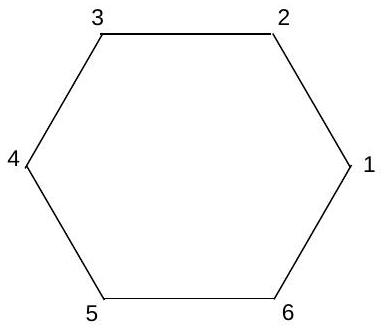
\includegraphics[max width=\textwidth, center]{2025_09_05_3ba26226ec0baddb5a03g-45}

Si ahora consideramos el conjunto $H_{n}$ de todas las permutaciones de los vértices que resultan como consecuencia de cada una de estas rotaciones, observamos que $H_{n}$ es el subgrupo de $S_{n}$ generado por la permutación $\rho=(123 \ldots n)$ (que es la permutación de los vértices que corresponde a la rotación del polígono en dirección antihoraria en un ángulo de $\frac{2 \pi}{n}$ ), es decir, $H_{n}=\left\{\rho, \rho^{2}, \rho^{3}, \ldots, \rho^{n}\right\}$. Llamaremos a $H_{n}$ el grupo cíclico de orden $n$. Por ejemplo, para $n=5$ se tiene que

$$
H_{5}=\left\{\left(\begin{array}{lllll}
1 & 2 & 3 & 4 & 5
\end{array}\right),(13524),(14253),(15432),(1)(2)(3)(4)(5)\right\}
$$

y su indicador de ciclos es $Z_{H_{5}}=t_{1}{ }^{5}+4 t_{5}$.

En cambio, para $n=6$ se tiene que

$$
\begin{aligned}
H_{6}=\{ & (123456),(135)(246),(14)(25)(36),(153)(264), \\
& (165432),(1)(2)(3)(4)(5)(6)\}
\end{aligned}
$$

y su indicador de ciclos es $Z_{H_{6}}=t_{1}{ }^{6}+t_{2}{ }^{3}+2 t_{3}{ }^{2}+2 t_{6}$.\\
Consideremos ahora el caso general. Queremos hallar $Z_{H_{n}}$,\\
En primer lugar, para cada $m$ entre 1 y $n$, debemos conocer cómo es la estructura cíclica de $\rho^{m}$.\\
Sea $i$ cualquier vértice entre 1 y $n$. Notando que $\rho^{m}(i)$ es el resto de dividir por $n$ a $m+i$ se tiene que $\rho^{m}(i)=r_{n}(m+i), \rho^{m}\left(r_{n}(m+i)\right)=r_{n}\left(m+r_{n}(m+i)\right)=r_{n}(2 m+i)$, $\rho^{m}\left(r_{n}(2 m+i)\right)=r_{n}(3 m+i), \ldots$.\\
Luego, el ciclo de $\rho^{m}$ que contiene a $i$ es $\left(i \quad r_{n}(m+i) \quad r_{n}(2 m+i) \quad r_{n}(3 m+i) \cdots\right)$, de donde resulta que la longitud del ciclo de $\rho^{m}$ que contiene a $i$ es el menor $k$ tal que $r_{n}(k m+i)=i$, es decir, el menor $k \in \mathbb{N}$ tal que $k m+i \equiv i(n)$. Luego, la longitud del ciclo de $\rho^{m}$ que contiene a $i$ es el menor $k \in \mathbb{N}$ tal que $n \mid k m$.\\
Sea $d=(n: m)$ el máximo común divisor entre $n$ y $m$. Entonces $\frac{n}{d}$ es un número natural y $n \left\lvert\, \frac{n}{d} m\right.$ pues $\frac{n}{d} m=n \frac{m}{d}$ y $\frac{m}{d} \in \mathbb{Z}$. Además, si $r \in \mathbb{N}$ satisface que $n \mid r m$, entonces $\frac{n}{d} \left\lvert\, r \frac{m}{d}\right.$. Como $\frac{n}{d}$ y $\frac{m}{d}$ son coprimos esto implica que $\left.\frac{n}{d} \right\rvert\, r$ de donde $\frac{n}{d} \leq r$. Esto muestra que el mínimo $k \in \mathbb{N}$ tal que $n \mid k m$ es $k=\frac{n}{d}$.\\
Conclusión: todos los ciclos de $\rho^{m}$ tienen la misma longitud $k=\frac{n}{d}$. Por lo tanto, $\rho^{m}$ tiene $\frac{n}{k}=d$ ciclos de longitud $k=\frac{n}{d}$, donde $d=(n: m)$.\\
En particular, hemos probado que todos los elementos de $H_{n}$ tienen $\frac{n}{k}$ ciclos de longitud $k$ para algún $k \in \mathbb{N}$ que divide a $n$. Luego, para hallar $Z_{H_{n}}$ sólo nos queda determinar cuántos elementos de $H_{n}$ tienen $\frac{n}{k}$ ciclos de longitud $k$ para cada divisor positivo $k$ de $n$.\\
Sea $k$ un divisor positivo de $n$. Notemos que, para cada $m$ entre 1 y $n, \rho^{m}$ tiene $\frac{n}{k}$ ciclos de longitud $k$ si y sólo si $\frac{n}{k}=(n: m)$.\\
Afirmación: $\frac{n}{k}=(n: m)$ si y sólo si $m=a \frac{n}{k}$ con $a \in \mathbb{N}, a \leq k$ y $(a: k)=1$\\
En efecto, si $\frac{n}{k}=(n: m)$ entonces, $\left.\frac{n}{k} \right\rvert\, m$ y por lo tanto $m=a \frac{n}{k}$ para algún $a \in \mathbb{N}$. Además, como $m \leq n$ entonces $a \leq k$ y como $\frac{n}{k}=(n: m)$ entonces

$$
\frac{n}{k}=\left(n: a \frac{n}{k}\right)=\left(k \frac{n}{k}: a \frac{n}{k}\right)=\frac{n}{k}(a: k)
$$

y por lo tanto $(a: k)=1$.\\
Recíprocamente, si $m=a \frac{n}{k}$ con $a \in \mathbb{N}, a \leq k$ y $(a: k)=1$ entonces

$$
(n: m)=\left(n: a \frac{n}{k}\right)=\left(k \frac{n}{k}: a \frac{n}{k}\right)=\frac{n}{k}(a: k)=\frac{n}{k}
$$

Luego, la cantidad de elementos de $H_{n}$ que tienen $\frac{n}{k}$ ciclos de longitud $k$ es igual al cardinal del conjunto

$$
\{a \in \mathbb{N} / a \leq k \mathrm{y}(a: k)=1\}
$$

Por lo tanto, para cada divisor positivo $k$ de $n$ hay exactamente $\Phi(k)$ elementos de $H_{n}$ que tienen $\frac{n}{k}$ ciclos de longitud $k$, donde $\Phi$ denota la función de Euler. Luego, el indicador de ciclos de $H_{n}$ es

$$
Z_{H_{n}}\left(t_{1}, t_{2}, \ldots, t_{n}\right)=\sum_{k \mid n} \Phi(k) t_{k}{ }^{\frac{n}{k}}
$$

Ejemplo 4: El grupo dihedral de grado $n$.\\
Consideremos un polígono regular de $n$ vértices en el plano. Ahora estamos interesados en las rotaciones y reflexiones en el plano tales que la posición final del polígono coincide con su posición inicial.\\
Sabemos que hay $n$ rotaciones, que son las que se obtienen rotando el polígono en dirección antihoraria en un ángulo igual a $\frac{2 k \pi}{n}(k=1,2, \ldots, n)$. Veamos cuáles son las reflexiones. Para ello, primero numeremos consecutivamente a los vértices del polígono con los números $1,2, \ldots, n$. Por ejemplo, para $n=5$\\
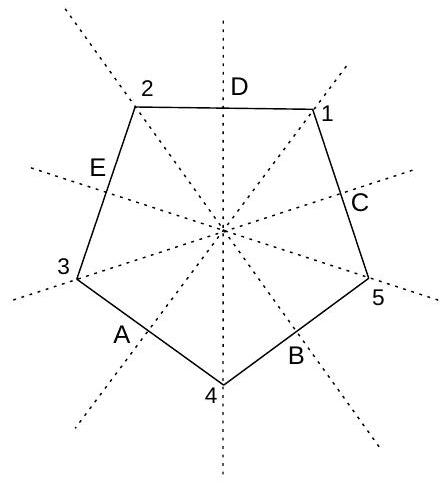
\includegraphics[max width=\textwidth, center]{2025_09_05_3ba26226ec0baddb5a03g-47}\\
hay 5 refexiones que son:\\
la reflexión respecto del eje 1 A (que permuta los vértices 3 y 4,2 y 5 y fija el vértice 1 la reflexión respecto del eje 2 B (que permuta los vértices 1 y 3,4 y 5 y fija el vértice 2 la reflexión respecto del eje 3 C (que permuta los vértices 2 y 4,1 y 5 y fija el vértice 3 la reflexión respecto del eje 4 D (que permuta los vértices 3 y 5,1 y 2 y fija el vértice 4 la reflexión respecto del eje 5 E (que permuta los vértices 1 y 4,2 y 3 y fija el vértice 5\\
y para $n=6$\\
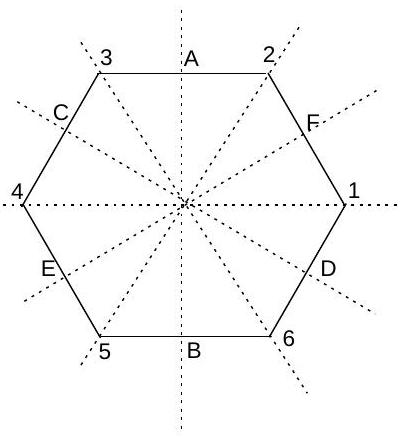
\includegraphics[max width=\textwidth, center]{2025_09_05_3ba26226ec0baddb5a03g-47(1)}\\
hay 6 reflexiones que son:\\
la reflexión respecto del eje 14 (que permuta los vértices 2 y 6,3 y 5 y fija los vértices 1 y 4)\\
la reflexión respecto del eje 25 (que permuta los vértices 1 y 3,4 y 6 y fija los vértices 2 y 5)\\
la reflexión respecto del eje 36 (que permuta los vértices 1 y 5,4 y 2 y fija los vértices 3 y 6)\\
la reflexión respecto del eje A B (que permuta los vértices 2 y 3,4 y 1 y 5 y 6 )\\
la reflexión respecto del eje C D (que permuta los vértices 4 y 3,6 y 1 y 5 y 2 )\\
la reflexión respecto del eje E F (que permuta los vértices 2 y 1,4 y 5 y 3 y 6 )\\
En general, un polígono regular de $n$ lados tiene $n$ reflexiones. Si $n$ es impar, estas son las reflexiones respecto del eje que pasa por un vértice y el punto medio del lado opuesto (que son $n)$ y, si $n$ es par, son las reflexiones respecto del eje que pasa por un par de vértices opuestos (de las cuales hay $\frac{n}{2}$ ) y las reflexiones respecto del eje que pasa por los puntos medios de un par de lados opuestos (de las cuales también hay $\frac{n}{2}$ ).\\
Sea $D_{n}$ el conjunto de todas las permutaciones de los vértices que resultan como consecuencia de cada una de las rotaciones o reflexiones del polígono regular de $n$ lados. Dejamos como ejercicio verificar que $D_{n}$ es un subgrupo de $S_{n}$ que tiene $2 n$ elementos, al que llamaremos el grupo dihedral de grado $n$.\\
Por ejemplo, para $n=5$ se tiene que

$$
\begin{aligned}
& D_{5}=\{(12345),(13524),(14253),(15432),(1)(2)(3)(4)(5), \\
& \quad(14)(23)(5),(13)(45)(2),(12)(53)(4),(34)(25)(1),(15)(24)(3)\}
\end{aligned}
$$

y para $n=6$ se tiene que

$$
\begin{aligned}
D_{6}=\{ & (123456),(135)(246),(14)(25)(36),(153)(264), \\
& (165432),(1)(2)(3)(4)(5)(6),(26)(35)(1)(4), \\
& (13)(46)(2)(5),(15)(42)(3)(6),(23)(14)(56), \\
& (43)(16)(52),(12)(45)(36)\}
\end{aligned}
$$

Calculemos ahora $Z_{D_{n}}$. Si consideramos las permutaciones de $D_{n}$ correspondientes a rotaciones, sabemos que para cada divisor positivo $k$ de $n$ hay exactamente $\Phi(k)$ de ellas que tienen $\frac{n}{k}$ ciclos de longitud $k$, donde $\Phi$ denota la función de Euler. Veamos qué ocurre con las reflexiones.

Si $n$ es impar, entonces cada reflexión permuta cada uno de los $\frac{n-1}{2}$ vértices que quedan de un lado del eje de reflexión con su opuesto respecto del eje y deja fijo un vértice que es el que está ubicado sobre el eje. En este caso, los $n$ elementos de $D_{n}$ correspondientes a\\
las reflexiones tienen $\frac{n-1}{2}$ ciclos del longitud 2 y un ciclo de longitud 1 . Por ejemplo, para $n=5$, las 5 permutaciones de $D_{5}$ correspondientes a reflexiones son

$$
(14)(23)(5),(13)(45)(2),(12)(53)(4),(34)(25)(1),(15)(24)(3)
$$

y todas ellas tienen $\frac{5-1}{2}=2$ ciclos de longitud 2 y un ciclo de longitud 1 .\\
Luego, si $n$ es impar, el indicador de ciclos de $D_{n}$ es

$$
n t_{1} t_{2}^{\frac{n-1}{2}}+\sum_{k \mid n} \Phi(k) t_{k}^{\frac{n}{k}}
$$

Por ejemplo, el indicador de ciclos de $D_{5}$ es $Z_{D_{5}}=5 t_{1} t_{2}{ }^{2}+t_{1}{ }^{5}+4 t_{5}$.\\
En cambio, si $n$ es par, las $\frac{n}{2}$ reflexiones respecto del eje que pasa por un par de vértices opuestos permutan los $\frac{n-2}{2}$ vértices que quedan de un lado del eje de reflexión con su opuesto respecto del eje y deja fijos dos vértices, que son los que están ubicados sobre el eje y las $\frac{n}{2}$ reflexiones respecto del eje que pasa por los puntos medios de un par de lados opuestos permutan los $\frac{n}{2}$ vértices que quedan de un lado del eje de reflexión con su opuesto respecto del eje. En este caso, de los $n$ elementos de $D_{n}$ correspondientes a las reflexiones, $\frac{n}{2}$ de ellos tienen $\frac{n-2}{2}$ ciclos del longitud 2 y dos ciclos de longitud 1 y los restantes $\frac{n}{2}$ tienen $\frac{n}{2}$ ciclos de longitud 2. Por ejemplo, para $n=6$, las 6 permutaciones de $D_{6}$ correspondientes a reflexiones son

$$
\begin{gathered}
(26)(35)(1)(4),(13)(46)(2)(5),(15)(42)(3)(6), \\
\quad(23)(14)(56),(43)(16)(52),(12)(45)(36)
\end{gathered}
$$

las tres primeras tienen $\frac{6-2}{2}=2$ ciclos de longitud 2 y dos de longitud 1 y las otras tres tienen $\frac{6}{2}=3$ ciclos de longitud 2 .\\
Luego, si $n$ es par, el indicador de ciclos de $D_{n}$ es

$$
\frac{n}{2} t_{1}^{2} t_{2}^{\frac{n-2}{2}}+\frac{n}{2} t_{2}^{\frac{n}{2}}+\sum_{k \mid n} \Phi(k) t_{k}^{\frac{n}{k}}
$$

Por ejemplo, para $n=6$ el indicador de ciclos de $D_{6}$ es

$$
Z_{D_{6}}=3 t_{1}^{2} t_{2}^{2}+3 t_{2}^{3}+t_{1}^{6}+t_{2}^{3}+2 t_{3}^{2}+2 t_{6}=3 t_{1}^{2} t_{2}^{2}+4 t_{2}^{3}+t_{1}^{6}+2 t_{3}^{3}+2 t_{6}
$$

En resumen,

$$
Z_{D_{n}}\left(t_{1}, t_{2}, \ldots, t_{n}\right)= \begin{cases}n t_{1} t_{2}^{\frac{n-1}{2}}+\sum_{k \mid n} \Phi(k) t_{k}^{\frac{n}{k}} & \text { si } n \text { es impar } \\ \frac{n}{2} t_{1}{ }^{2} t_{2}^{\frac{n-2}{2}}+\frac{n}{2} t_{2}^{\frac{n}{2}}+\sum_{k \mid n} \Phi(k) t_{k}{ }^{\frac{n}{k}} & \text { si } n \text { es par }\end{cases}
$$

\section*{Teorema de Burnside.}
Comenzaremos esta sección con un ejemplo. Hay 16 maneras de pintar los vértices de un cuadrado con dos colores, blanco y negro, que son\\
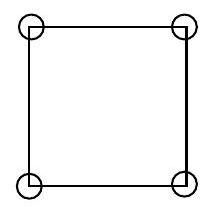
\includegraphics[max width=\textwidth, center]{2025_09_05_3ba26226ec0baddb5a03g-50(10)}\\
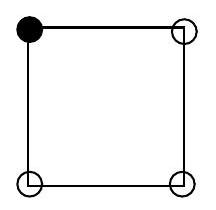
\includegraphics[max width=\textwidth, center]{2025_09_05_3ba26226ec0baddb5a03g-50(4)}\\
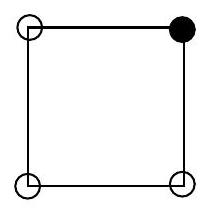
\includegraphics[max width=\textwidth, center]{2025_09_05_3ba26226ec0baddb5a03g-50(14)}\\
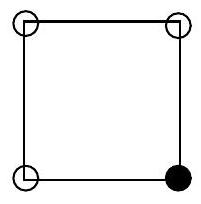
\includegraphics[max width=\textwidth, center]{2025_09_05_3ba26226ec0baddb5a03g-50(6)}\\
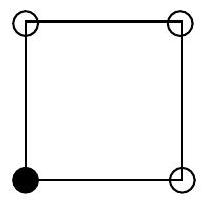
\includegraphics[max width=\textwidth, center]{2025_09_05_3ba26226ec0baddb5a03g-50(8)}\\
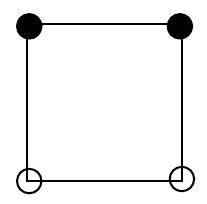
\includegraphics[max width=\textwidth, center]{2025_09_05_3ba26226ec0baddb5a03g-50(1)}\\
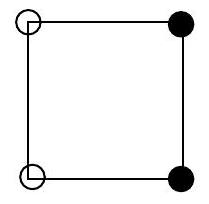
\includegraphics[max width=\textwidth, center]{2025_09_05_3ba26226ec0baddb5a03g-50(5)}\\
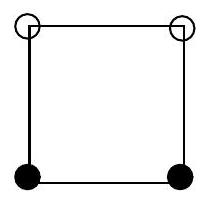
\includegraphics[max width=\textwidth, center]{2025_09_05_3ba26226ec0baddb5a03g-50(13)}\\
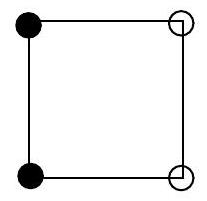
\includegraphics[max width=\textwidth, center]{2025_09_05_3ba26226ec0baddb5a03g-50(3)}\\
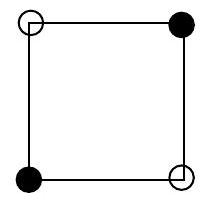
\includegraphics[max width=\textwidth, center]{2025_09_05_3ba26226ec0baddb5a03g-50}\\
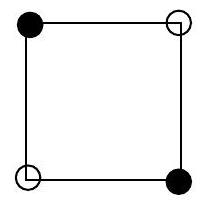
\includegraphics[max width=\textwidth, center]{2025_09_05_3ba26226ec0baddb5a03g-50(9)}\\
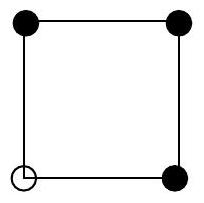
\includegraphics[max width=\textwidth, center]{2025_09_05_3ba26226ec0baddb5a03g-50(11)}\\
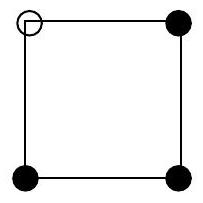
\includegraphics[max width=\textwidth, center]{2025_09_05_3ba26226ec0baddb5a03g-50(15)}\\
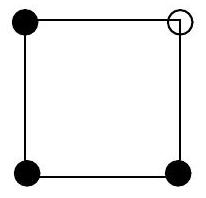
\includegraphics[max width=\textwidth, center]{2025_09_05_3ba26226ec0baddb5a03g-50(2)}\\
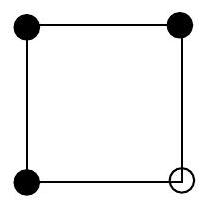
\includegraphics[max width=\textwidth, center]{2025_09_05_3ba26226ec0baddb5a03g-50(7)}\\
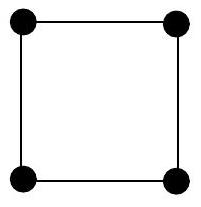
\includegraphics[max width=\textwidth, center]{2025_09_05_3ba26226ec0baddb5a03g-50(12)}

Como se observa, las 16 figuras se agrupan en 6 clases. Las figuras de cada clase pueden obtenerse unas de otras aplicando alguna de las cuatro rotaciones del cuadrado. Por lo tanto, si consideramos equivalentes dos figuras cuando una de ellas se obtiene de la otra por una rotación del cuadrado, entonces hay sólo 6 figuras no equivalentes.

Si numeramos los vértices del cuadrado en la forma\\
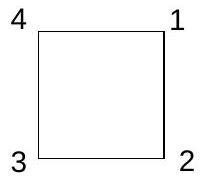
\includegraphics[max width=\textwidth, center]{2025_09_05_3ba26226ec0baddb5a03g-51(2)}\\
cada figura se puede identificar con una función $f:\{1,2,3,4\} \longrightarrow\{B, N\}$ que asigna a cada uno de los cuatro vértices $B$ o $N$ según el vértice sea blanco o negro. Componiendo una permutación de $S_{4}$ correspondiente a una rotación del cuadrado con una de estas funciones (que representa una figura) obtenemos otra función (que representa otra de las figuras de su misma clase). De esta manera, la clase de equivalencia de una figura se obtiene componiendo cada una de las permutación de $S_{4}$ que corresponden a una rotación del cuadrado con la función que representa a dicha figura. Esto nos permite expresar analíticamente el concepto geométrico de rotar la figura en otra equivalente. Por ejemplo, componiendo la permutación $\rho=\left(\begin{array}{llll}1 & 2 & 3 & 4\end{array}\right)$, correspondiente a la rotación en sentido horario de $90^{0}$, con la función $f$ definida por $f(1)=N, f(2)=N, f(3)=B, f(4)=N$ que representa la figura\\
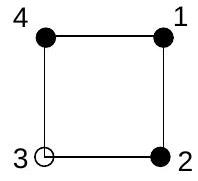
\includegraphics[max width=\textwidth, center]{2025_09_05_3ba26226ec0baddb5a03g-51(3)}\\
obtenemos la función $g=f \rho$ definida por $g(1)=N, g(2)=B, g(3)=N, g(4)=N$ que representa la figura (equivalente a la anterior)\\
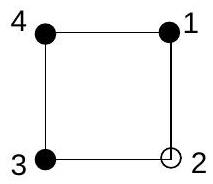
\includegraphics[max width=\textwidth, center]{2025_09_05_3ba26226ec0baddb5a03g-51(1)}\\
es decir, $\rho$ transforma la primera figura en la segunda figura\\
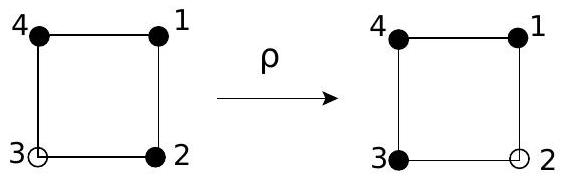
\includegraphics[max width=\textwidth, center]{2025_09_05_3ba26226ec0baddb5a03g-51}

Si $X$ es un conjunto, denotaremos por $S_{X}$ al conjunto

$$
S_{X}=\{\pi: X \longrightarrow X / \pi \text { es biyectiva }\}
$$

A los elementos de $S_{X}$ los llamaremos permutaciones de $X$. Dejamos como ejercicio mostrar que $S_{X}$ es un grupo con la composición de funciones. Si, además, $X$ es finito entonces $S_{X}$ es un grupo finito.

Teorema de Burnside: Sea $X$ un conjunto finito y sea $G$ un subgrupo de $S_{X}$. Sea $K$ un conjunto finito y sea $F$ un subconjunto de funciones de $X$ en $K$.\\
Sea $\sim$ la relación de equivalencia en $F$ definida por

$$
f \sim g \quad \Longleftrightarrow \quad \exists \pi \in G / g=f \pi
$$

Entonces la cantidad de clases de equivalencia es

$$
\nu=\frac{1}{|G|} \sum_{\pi \in G}|\{f \in F / f \pi=f\}|
$$

Demostración: Veremos primero que si $f$ y $g$ pertenecen a la misma clase de equivalencia, entonces $|\{\pi \in G / f \pi=g\}|=|\{\sigma \in G / g \sigma=g\}|$. Sea $\tau \in G$ tal que $f=g \tau$. Entonces la aplicación $h:\{\pi \in G / f \pi=g\} \longrightarrow\{\sigma \in G / g \sigma=g\}$ definida por $h(\pi)=\tau \pi$ es una biyección.\\
En primer lugar, notemos que dada $\pi \in G$ tal que $f \pi=g$, como $f=g \tau$ entonces $h(\pi)=\tau \pi \in G$ y satisface $g h(\pi)=g \tau \pi=f \pi=g$, es decir, $h$ está bien definida. Además, $h$ es inyectiva pues

$$
h(\pi)=h\left(\pi^{\prime}\right) \Longrightarrow \tau \pi=\tau \pi^{\prime} \Longrightarrow \pi=\pi^{\prime}
$$

y es suryectiva pues dada $\sigma \in G$ tal que $g \sigma=g$, tomando $\pi=\tau^{-1} \sigma$ resulta que $\pi \in G$ y

$$
f \pi=f \tau^{-1} \sigma=g \sigma=g \text { y } h(\pi)=\tau \tau^{-1} \sigma=\sigma
$$

Si $\mathcal{C}=\left\{f_{1}, f_{2}, \ldots, f_{s}\right\}$ es una clase de equivalencia de $F$ entonces, dada $\pi \in G, f_{1} \pi$ es equivalente a $f_{1}$ y por lo tanto $f_{1} \pi \in \mathcal{C}$, de donde $f_{1} \pi=f_{i}$ para algún $i$ entre 1 y $s$. Luego

$$
G=\bigcup_{i=1}^{s}\left\{\pi \in G / f_{1} \pi=f_{i}\right\}
$$

y esta unión es claramente disjunta.\\
Por lo tanto, usando lo que probamos antes, resulta que

$$
|G|=\sum_{i=1}^{s}\left|\left\{\pi \in G / f_{1} \pi=f_{i}\right\}\right|=\sum_{i=1}^{s}\left|\left\{\pi \in G / f_{i} \pi=f_{i}\right\}\right|=\sum_{f \in \mathcal{C}}|\{\pi \in G / f \pi=f\}|
$$

Sean $\mathcal{C}_{1}, \mathcal{C}_{2}, \ldots, \mathcal{C}_{\nu}$ las clases de equivalencia de $F$. Ahora, definiendo para cada $f \in F$, $\pi \in G$,

$$
\delta(f, \pi)= \begin{cases}1 & \text { si } f \pi=f \\ 0 & \text { si no }\end{cases}
$$

y usando que

$$
\sum_{\pi \in G} \sum_{f \in F} \delta(f, \pi)=\sum_{f \in F} \sum_{\pi \in G} \delta(f, \pi)
$$

y que $F$ es la unión disjunta de sus clases de equivalencia, obtenemos que

$$
\begin{aligned}
& \sum_{\pi \in G}|\{f \in F / f \pi=f\}|=\sum_{\pi \in G} \sum_{f \in F} \delta(f, \pi)=\sum_{f \in F} \sum_{\pi \in G} \delta(f, \pi)=\sum_{f \in F}|\{\pi \in G / f \pi=f\}|= \\
& =\sum_{f \in \mathcal{C}_{1}}|\{\pi \in G / f \pi=f\}|+\sum_{f \in \mathcal{C}_{2}}|\{\pi \in G / f \pi=f\}|+\cdots+\sum_{f \in \mathcal{C}_{\nu}}|\{\pi \in G / f \pi=f\}|= \\
& =|G|+|G|+\cdots+|G|=\nu|G|
\end{aligned}
$$

Luego,

$$
\nu=\frac{1}{|G|} \sum_{\pi \in G}|\{f \in F / f \pi=f\}|
$$

como queríamos probar. ㅁ\\
En el ejemplo de pintar los vértices de un cuadrado de blanco o de negro, se tiene que $K=\{B, N\}, X=\{1,2,3,4\}$ es el conjunto de vértices del cuadrado, y cada elemento $f$ de $F$ es una función $f: X \longrightarrow K$ que representa una coloración de los vértices del cuadrado, es decir, una de las figuras. En este caso, $G$ es el subgrupo de 4 elementos de $S_{4}$

$$
G=\{(1)(2)(3)(4),(1234),(13)(24),(1432)\}
$$

que representa cada una de las 4 rotaciones del cuadrado:\\
$\pi=(1)(2)(3)(4)$, que representa una rotación de $0^{0}$, deja fijas las 16 figuras\\
$\pi=\left(\begin{array}{lll}1 & 2 & 3\end{array}\right)$, que representa la rotación de $90^{\circ}$ en sentido horario, deja fijas sólo 2 figuras: la que tiene todos sus vértices blancos y la que tiene todos sus vértices negros.\\
$\pi=(13)(24)$, que representa la rotación de $180^{\circ}$ en el sentido horario, deja fijas las 4 figuras\\
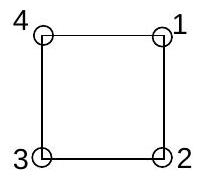
\includegraphics[max width=\textwidth, center]{2025_09_05_3ba26226ec0baddb5a03g-53(2)}\\
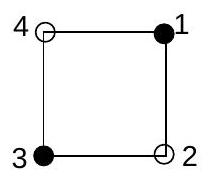
\includegraphics[max width=\textwidth, center]{2025_09_05_3ba26226ec0baddb5a03g-53}\\
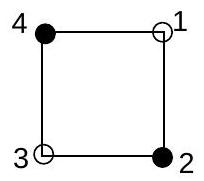
\includegraphics[max width=\textwidth, center]{2025_09_05_3ba26226ec0baddb5a03g-53(1)}\\
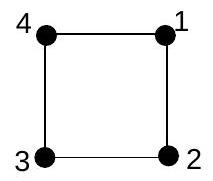
\includegraphics[max width=\textwidth, center]{2025_09_05_3ba26226ec0baddb5a03g-53(3)}\\
y $\pi=\left(\begin{array}{lll}1 & 4 & 3\end{array}\right)$, que representa la rotación de $270^{\circ}$ en sentido horario, deja fijas sólo 2 figuras: la que tiene todos sus vértices blancos y la que tiene todos sus vértices negros.\\
Luego, hay $\frac{1}{4}(16+2+4+2)=6$ clases de equivalencia.\\
En general, si el conjunto finito $K$ es un conjunto de colores y cada $f: X \longrightarrow K$ es una coloración de los elementos de $X(f(x)$ es el color con el cual pintamos al elemento $x)$ nos preguntamos si, al aplicar una permutación a los elementos de $X$, el color asignado a\\
cada elemento de $X$ no ha cambiado (es decir, si la permutación deja fija la figura a la que representa $f$ ).\\
Por ejemplo, si $X$ es un conjunto de 8 elementos, pintamos los elementos 1, 2, 6 y 7 de blanco y los restantes de negro en la forma\\
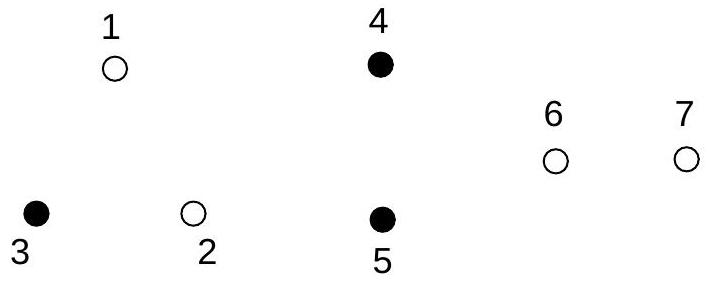
\includegraphics[max width=\textwidth, center]{2025_09_05_3ba26226ec0baddb5a03g-54(2)}\\
la función $f$ es la definida por

$$
f(1)=f(2)=f(6)=f(7)=B \text { y } f(3)=f(4)=f(5)=f(8)=N
$$

si ahora aplicamos la permutación $\pi=\left(\begin{array}{lll}1 & 2 & 3\end{array}\right)\left(\begin{array}{ll}4 & 5\end{array}\right)\left(\begin{array}{ll}6 & 7\end{array}\right)(8)$, se tiene que $f \pi(1)=B$, $f \pi(2)=N, f \pi(3)=B, f(4)=N, f(5)=N, f(6)=B, f(7)=B$ y $f(8)=N$. Por lo tanto, la figura resultante es\\
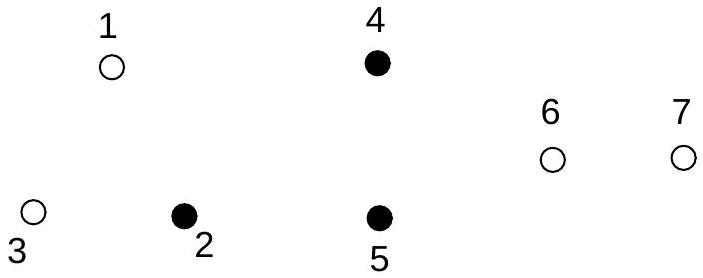
\includegraphics[max width=\textwidth, center]{2025_09_05_3ba26226ec0baddb5a03g-54(1)}\\
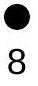
\includegraphics[max width=\textwidth, center]{2025_09_05_3ba26226ec0baddb5a03g-54}

Observamos que para que no cambie ninguno de los colores asignados a los elementos de $X$ al aplicar la permutación $\pi$, los elementos de un mismo ciclo de $\pi$ deberían ser todos del mismo color. En esta figura esto no ocurre para el ciclo ( 123 ) y eso produce que los elementos 1,2 y 3 no conserven su color al aplicar $\pi$. Luego, la figura no queda fija por $\pi$.

Lema: Sea $\pi$ una permutación de un conjunto finito $X$ y sea $f$ una función de $X$ en un conjunto finito $K$. Entonces $f \pi=f$ si y sólo $f(x)=f(y)$ para todo par de elementos $x, y$ de $X$ que pertenezcan a un mismo ciclo de $\pi$.

Demostración: $(\Leftarrow)$ Supongamos que $f(x)=f(y)$ para todo par de elementos $x, y$ de $X$ que pertenezcan a un mismo ciclo de $\pi$.\\
Dado $x \in X$, debemos ver que $(f \pi)(x)=f(x)$. Sea $y=\pi(x)$. Entonces $x$ e $y$ pertenecen al mismo ciclo de $\pi$. Luego $f(x)=f(y)=(f \pi)(x)$.\\
$(\Rightarrow)$ Supongamos ahora que $(f \pi)(x)=f(x)$ para todo $x \in X$. Si ( $x_{1} \quad x_{2} \quad \ldots, x_{s}$ ) es un ciclo de $\pi$ entonces $f\left(x_{2}\right)=(f \pi)\left(x_{1}\right)=f\left(x_{1}\right), f\left(x_{3}\right)=(f \pi)\left(x_{2}\right)=f\left(x_{2}\right)=f\left(x_{1}\right)$, $f\left(x_{4}\right)=(f \pi)\left(x_{3}\right)=f\left(x_{3}\right)=f\left(x_{1}\right), \ldots, f\left(x_{s}\right)=(f \pi)\left(x_{s-1}\right)=f\left(x_{s-1}\right)=f\left(x_{1}\right)$. Luego, $f\left(x_{1}\right)=f\left(x_{2}\right)=\ldots=f\left(x_{s}\right)$.

Supongamos ahora que $X=\{1,2, \ldots, n\}, K$ es un conjunto de $m$ elementos y $F$ es el conjunto de todas las funciones de $X$ en $K$.\\
Dada una permutación $\pi$ de $X$ (es decir, un elemento de $S_{n}$ ) queremos determinar cuántas funciones de $X$ en $K$ quedan fijas por $\pi$, es decir, $|\{f \in F / f \pi=f\}|$.\\
Por ejemplo, si $X=\{1,2,3,4,5,6,7,8,9\}$ y $\pi=(13)(24)(5)(6)(789)$ entonces $f \in F$ queda fija por $\pi$ si y sólo si $f(1)=f(3), f(2)=f(4), f(7)=f(8)=f(9)$. Luego, hay exactamente $m^{5}$ funciones de $X$ en $K$ que quedan fijas por $\pi$.\\
En general, si $\pi$ tiene $\lambda_{1}(\pi)$ ciclos de longitud $1, \lambda_{2}(\pi)$ ciclos de longitud $2, \ldots, \lambda_{n}(\pi)$ ciclos de longitud $n$ entonces la cantidad de funciones que quedan fijas por $\pi$ es

$$
|\{f \in F / f \pi=f\}|=m^{\lambda_{1}(\pi)+\lambda_{2}(\pi)+\cdots+\lambda_{n}(\pi)}=m^{\lambda_{1}(\pi)} m^{\lambda_{2}(\pi)} \ldots m^{\lambda_{n}(\pi)}
$$

Luego, si $F$ es el conjunto de todas las funciones de $X=\{1,2, \ldots, n\}$ en $K, G$ es un subgrupo de $S_{n}$ y $\sim$ es la relación de equivalencia en $F$ definida por

$$
f \sim g \quad \Longleftrightarrow \quad \exists \pi \in G / g=f \pi
$$

Entonces, aplicando el teorema de Burnside y teniendo en cuenta que

$$
Z_{G}\left(t_{1}, t_{2}, \ldots, t_{n}\right)=\sum_{\pi \in G} t_{1}^{\lambda_{1}(\pi)} t_{2}^{\lambda_{2}(\pi)} \ldots t_{n}^{\lambda_{n}(\pi)}
$$

resulta que la cantidad de clases de equivalencia es

$$
\begin{aligned}
\nu & =\frac{1}{|G|} \sum_{\pi \in G}|\{f \in F / f \pi=f\}|= \\
& =\frac{1}{|G|} \sum_{\pi \in G} m^{\lambda_{1}(\pi)} m^{\lambda_{2}(\pi)} \ldots m^{\lambda_{n}(\pi)}= \\
& =\frac{1}{|G|} Z_{G}(m, m, \ldots, m)
\end{aligned}
$$

Hemos demostrado entonces el siguiente corolario del teorema de Burnside\\
Corolario: Si $F$ es el conjunto de todas las funciones de $X=\{1,2, \ldots, n\}$ en un conjunto finito $K, G$ es un subgrupo de $S_{n}$ y $\sim$ es la relación de equivalencia en $F$ definida por

$$
f \sim g \quad \Longleftrightarrow \quad \exists \pi \in G / g=f \pi
$$

entonces la cantidad de clases de equivalencia es $\nu=\frac{1}{|G|} Z_{G}(|K|,|K|, \ldots,|K|)$, donde $Z_{G}\left(t_{1}, t_{2}, \ldots, t_{n}\right)$ es el indicador de ciclos de $G$.

Ejemplo 1: Si pintamos los vértices de un pentágono de blanco, negro, amarillo o rojo y consideramos que dos figuras son equivalentes si una se obtiene de la otra por una rotación\\
del pentágono, entonces la cantidad de clases de equivalencia es $\frac{1}{|G|} Z_{G}(4,4,4,4,4)$, donde $G=H_{5}$. Como $|G|=5$ y $Z_{G}=t_{1}^{5}+4 t_{5}$ entonces la cantidad de clases de equivalencia es

$$
\frac{4^{5}+4.4}{5}=208
$$

Ejemplo 2: ¿Cuántos collares de 8 cuentas se pueden obtener si se utilizan cuentas rojas, verdes o amarillas?\\
Esto es lo mismo que determinar de cuántas maneras se pueden pintar los vértices numerados de un octógono regular con tres colores, considerando equivalentes las figuras que quedan fijas por las rotaciones y reflexiones del octógono.\\
En este ejemplo, $X=\{1,2, \ldots, 8\}, F$ es el conjunto de todas las funciones de $X$ en $K=\{R, V, A\}$ (es decir, todas las maneras de colorear los vértices con los colores dados) y $G=D_{8}$ es el grupo dihedral de rotaciones y reflexiones del octógono regular, que es un subgrupo de $S_{8}$ de $2.8=16$ elementos.\\
Teniendo en cuenta que el indicador de ciclos de $D_{8}$ es

$$
Z_{D_{8}}=4 t_{1}^{2} t_{2}^{3}+5 t_{2}^{4}+t_{1}^{8}+2 t_{4}^{2}+4 t_{8}
$$

se tiene entonces que la cantidad de collares, que es igual a la cantidad de clases de equivalencia, es

$$
\begin{aligned}
& \frac{1}{\left|D_{8}\right|} Z_{D_{8}}(|K|,|K|, \ldots,|K|)= \\
& \quad=\frac{1}{16}\left(4.3^{2} 3^{3}+5.3^{4}+3^{8}+2.3^{2}+4.3\right)= \\
& \quad=\frac{1}{16}\left(4.3^{5}+5.3^{4}+3^{8}+2.3^{2}+4.3\right)
\end{aligned}
$$

\section*{Teorema de Polya.}
Supongamos que pintamos los vértices de un cuadrado de blanco o negro, y consideramos que dos figuras son equivalentes si una se obtiene de la otra por una rotación del cuadrado. Como ya vimos, esto parte al conjunto de figuras en las 6 clases de equivalencia\\
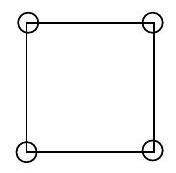
\includegraphics[max width=\textwidth, center]{2025_09_05_3ba26226ec0baddb5a03g-56(2)}\\
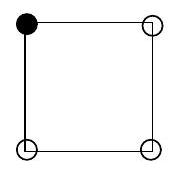
\includegraphics[max width=\textwidth, center]{2025_09_05_3ba26226ec0baddb5a03g-56(5)}\\
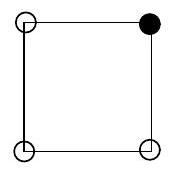
\includegraphics[max width=\textwidth, center]{2025_09_05_3ba26226ec0baddb5a03g-56}\\
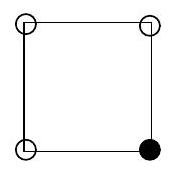
\includegraphics[max width=\textwidth, center]{2025_09_05_3ba26226ec0baddb5a03g-56(6)}\\
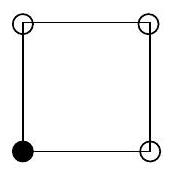
\includegraphics[max width=\textwidth, center]{2025_09_05_3ba26226ec0baddb5a03g-56(3)}\\
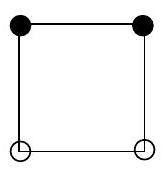
\includegraphics[max width=\textwidth, center]{2025_09_05_3ba26226ec0baddb5a03g-56(4)}\\
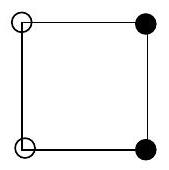
\includegraphics[max width=\textwidth, center]{2025_09_05_3ba26226ec0baddb5a03g-56(1)}\\
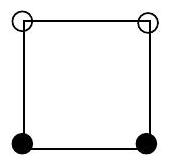
\includegraphics[max width=\textwidth, center]{2025_09_05_3ba26226ec0baddb5a03g-56(8)}\\
\includegraphics[max width=\textwidth, center]{2025_09_05_3ba26226ec0baddb5a03g-56(7)}\\
\includegraphics[max width=\textwidth, center]{2025_09_05_3ba26226ec0baddb5a03g-57(2)}

Notemos que si dos figuras pertenecen a la misma clase de equivalencia entonces tienen la misma cantidad de vértices negros y la misma cantidad de vértices blancos. Sin embargo, la recíproca no es cierta. Por ejemplo, las figuras\\
\includegraphics[max width=\textwidth, center]{2025_09_05_3ba26226ec0baddb5a03g-57(1)}\\
\includegraphics[max width=\textwidth, center]{2025_09_05_3ba26226ec0baddb5a03g-57}\\
no pertenecen a la misma clase de equivalencia pero ambas tienen dos vértices negros y dos blancos.\\
Si llamamos $c\left(k_{1}, k_{2}\right)$ a la cantidad de clases de equivalencia cuyas figuras tienen $k_{1}$ vértices blancos y $k_{2}$ negros, se tiene entonces que $c(4,0)=1, c(3,1)=1 . c(2,2)=2, c(1,3)=1$, $c(0,4)=1$ y $c\left(k_{1}, k_{2}\right)=0$ si $k_{1}+k_{2} \neq 4$\\
En general, si $G$ es un subgrupo de $S_{n}$ y $F$ es el conjunto de todas las funciones de $X=\{1,2, \ldots, n\}$ en un conjunto finito $K=\left\{c_{1}, c_{2}, \ldots, c_{m}\right\}$ y consideramos la la relación de equivalencia $\sim$ en $F$ definida por

$$
f \sim g \quad \Longleftrightarrow \quad \exists \pi \in G / g=f \pi
$$

resulta que si $f$ y $g$ están en la misma clase de equivalencia entonces $\left|f^{-1}\left(c_{i}\right)\right|=\left|g^{-1}\left(c_{i}\right)\right|$ para todo $i$ entre 1 y $m$.\\
Sin embargo, tal como pasaba en el ejemplo anterior, si $k_{i}=\left|f^{-1}\left(c_{i}\right)\right|$ (es decir, si f toma $k_{1}$ valores iguales a $c_{1}, k_{2}$ valores iguales a $c_{2}, \ldots, k_{m}$ valores iguales a $c_{m}$ ) puede haber funciones que estén en clases de equivalencia distintas de la clase de $f$ que también tomen $k_{1}$ valores iguales a $c_{1}, k_{2}$ valores iguales a $c_{2}, \ldots, k_{m}$ valores iguales a $c_{m}$. Nos preguntamos, para cada $k_{1}, k_{2}, \ldots, k_{m}$, cuál es la cantidad $c\left(k_{1}, k_{2}, \ldots, k_{m}\right)$ de clases de equivalencia cuyos elementos toman $k_{1}$ valores iguales a $c_{1}, k_{2}$ valores iguales a $c_{2}, \ldots, k_{m}$ valores iguales a $c_{m}$. Claramente, este número será cero si $k_{1}+k_{2}+\cdots+k_{m} \neq n$, por lo que supondremos que $k_{1}+k_{2}+\cdots+k_{m}=n$.

Para cacular este número, hallaremos el polinomio en las $m$ indeterminadas $c_{1}, c_{2}, \ldots, c_{m}$,

$$
\sum_{k_{1}+k_{2}+\cdots+k_{m}=n} c\left(k_{1}, k_{2}, \ldots, k_{m}\right) c_{1}^{k_{1}} c_{2}^{k_{2}} \ldots c_{m}^{k_{m}}
$$

A este polinomio lo llamaremos el inventario de funciones equivalentes. Por ejemplo, si $G$ es el grupo cíclico de orden 4 (que representa las rotaciones del cuadrado) y $K=\{b, n\}$, el inventario de funciones equivalentes es $b^{4}+b^{3} n+2 b^{2} n^{2}+b n^{3}+n^{4}$.

Ejemplo: Supongamos que pintamos los vértices de un hexágono con 3 colores, $a, b$ y $c$ y consideramos que dos figuras son equivalentes si una se obtiene de la otra por una rotación o una reflexión del hexágono. Nos preguntamos cuántas figuras no equivalentes hay que tengan $k_{1}$ vértices del color $a, k_{2}$ vértices del color $b$ y $k_{3}$ vértices del color $c$, donde $k_{1}+k_{2}+k_{3}=6$.\\
En este caso, $F$ es el conjunto de todas las funciones de $X=\{1,2, \ldots, 6\}$ en $K=\{a, b, c\}$ y $G=D_{6}$ y estamos considerando que dos funciones $f$ y $g$ son equivalentes si $f=g \pi$ para algún $\pi \in G$. Queremos determinar la cantidad $c\left(k_{1}, k_{2}, k_{3}\right)$ de clases de equivalencia tales que sus elementos toman $k_{1}$ valores iguales a $a, k_{2}$ valores iguales a $b$ y $k_{3}$ valores iguales a $c$.\\
Notemos que esto es lo mismo que hallar primero todas las figuras que tienen $k_{1}$ vértices del color $a, k_{2}$ vértices del color $b$ y $k_{3}$ vértices del color $c$ y luego clasificarlas en clases de equivalencia. La cantidad de clases de equivalencia será el número $c\left(k_{1}, k_{2}, k_{3}\right)$ que estamos buscando.\\
Sea $F^{\prime}$ el conjunto de todas las funciones que toman $k_{1}$ valores iguales a $a, k_{2}$ valores iguales a $b$ y $k_{3}$ valores iguales a $c$, es decir,

$$
F^{\prime}=\left\{f \in F /\left|f^{-1}(a)\right|=k_{1},\left|f^{-1}(b)\right|=k_{2} \text { y }\left|f^{-1}(c)\right|=k_{3}\right\}
$$

Si consideramos ahora la relación de equivalencia $\sim$ en $F^{\prime}$ definida por

$$
f \sim g \quad \Longleftrightarrow \quad \exists \pi \in G / g=f \pi
$$

entonces $c\left(k_{1}, k_{2}, k_{3}\right)$ es la cantidad de clases de equivalencia.\\
Por el teorema de Burnside, se tiene que

$$
c\left(k_{1}, k_{2}, k_{3}\right)=\frac{1}{|G|} \sum_{\pi \in G}\left|\left\{f \in F^{\prime} / f \pi=f\right\}\right|
$$

Sea $\pi \in G$. Recordemos que $f \in F^{\prime}$ satisface $f \pi=f$ si y sólo si $f$ es constante en cada ciclo de $\pi$. Supongamos que $\pi$ tiene $\lambda_{1}(\pi)$ ciclos de longitud $1, \lambda_{2}(\pi)$ ciclos de longitud 2 , $\ldots, \lambda_{6}(\pi)$ ciclos de longitud 6 . Entonces, si $c_{\pi}\left(k_{1}, k_{2}, k_{3}\right)=\left|\left\{f \in F^{\prime} / f \pi=f\right\}\right|$, se tiene que $c_{\pi}\left(k_{1}, k_{2}, k_{3}\right)$ es el coeficiente de $a^{k_{1}} b^{k_{2}} c^{k_{3}}$ del polinomio

$$
(a+b+c)^{\lambda_{1}(\pi)}\left(a^{2}+b^{2}+c^{2}\right)^{\lambda_{2}(\pi)}\left(a^{3}+b^{3}+c^{3}\right)^{\lambda_{3}(\pi)} \ldots\left(a^{6}+b^{6}+c^{6}\right)^{\lambda_{6}(\pi)}
$$

Por ejemplo, si $\pi=(2)$ (5) (13) (46), entonces $f \pi=f$ sii $f(1)=f(3)$ y $f(4)=f(6)$. En este caso el polinomio es

$$
(a+b+c)(a+b+c)\left(a^{2}+b^{2}+c^{2}\right)\left(a^{2}+b^{2}+c^{2}\right)
$$

Al calcular el coeficiente de $a^{3} b^{2} c$ aplicando la propiedad distributiva, vemos que hay 4 formas de obtener $a^{3} b^{2} c$ que son

$$
\left.\begin{array}{l}
\left(\begin{array}{lll} 
& c & )(a \\
(a & )( & a
\end{array}\right)\left(\begin{array}{ll}
b^{2} & ) \\
( & c)\left(a^{2}\right.
\end{array}\right)\left(\begin{array}{ll}
b^{2} & ) \\
(a & c)\left(b^{2}\right.
\end{array}\right)\left(a^{2}\right.
\end{array}\right)
$$

lo que se identifica con las coloraciones\\
pintar el vértice 2 del color $c$, el 5 de $a$, el 1 y el 3 de $a$, el 4 y 6 de $b$\\
pintar el vértice 2 del color $a$, el 5 de $c$, el 1 y el 3 de $a$, el 4 y 6 de $b$\\
pintar el vértice 2 del color $c$, el 5 de $a$, el 1 y el 3 de $b$, el 4 y 6 de $a$\\
pintar el vértice 2 del color $a$, el 5 de $c$, el 1 y el 3 de $b$, el 4 y 6 de $a$\\
es decir, con las funciones\\
$f(2)=c, f(5)=a, f(1)=f(3)=a, f(4)=f(6)=b$\\
$f(2)=a, f(5)=c, f(1)=f(3)=a, f(4)=f(6)=b$\\
$f(2)=c, f(5)=a, f(1)=f(3)=b, f(4)=f(6)=a$\\
$f(2)=a, f(5)=c, f(1)=f(3)=b, f(4)=f(6)=a$\\
que son todas las funciones que quedan fijas por $\pi$ y toman 3 valores $a, 2$ valores $b$ y un valor $c$, es decir, $c_{\pi}(3,2,1)=4$.\\
Y al calcular el coeficiente de $a b^{4} c$ aplicando la propiedad distributiva, vemos que hay 2 formas de obtener $a b^{4} c$ que son

$$
\left.\begin{array}{lll}
( & c)(a & )\left(\begin{array}{ll} 
& b^{2}
\end{array}\right)\left(\begin{array}{l}
b^{2}
\end{array}\right) \\
(a & )( & c)( \\
b^{2}
\end{array}\right)\left(\begin{array}{l}
b^{2}
\end{array}\right)
$$

lo que se identifica con las coloraciones\\
pintar el vértice 2 del color $c$, el 5 de $a$, el 1 y el 3 de $b$, el 4 y 6 de $b$\\
pintar el vértice 2 del color $a$, el 5 de $c$, el 1 y el 3 de $b$, el 4 y 6 de $b$\\
es decir, con las funciones\\
$f(2)=c, f(5)=a, f(1)=f(3)=b, f(4)=f(6)=b$\\
$f(2)=a, f(5)=c, f(1)=f(3)=b, f(4)=f(6)=b$\\
que son todas las funciones que quedan fijas por $\pi$ y toman un valor $a, 4$ valores $b$ y un valor $c$, es decir, $c_{\pi}(1,4,1)=2$.

Luego,

$$
(a+b+c)^{\lambda_{1}(\pi)}\left(a^{2}+b^{2}+c^{2}\right)^{\lambda_{2}(\pi)} \ldots\left(a^{6}+b^{6}+c^{6}\right)^{\lambda_{6}(\pi)}=\sum_{k_{1}+k_{2}+k_{3}=6} c_{\pi}\left(k_{1}, k_{2}, k_{3}\right) a^{k_{1}} b^{k_{2}} c^{k_{3}}
$$

Sumando sobre todo $\pi \in G$ y dividiendo por $|G|$ obtenemos

$$
\begin{aligned}
& \frac{1}{|G|} \sum_{\pi \in G}(a+b+c)^{\lambda_{1}(\pi)}\left(a^{2}+b^{2}+c^{2}\right)^{\lambda_{2}(\pi)} \ldots\left(a^{6}+b^{6}+c^{6}\right)^{\lambda_{6}(\pi)}= \\
& =\frac{1}{|G|} \sum_{\pi \in G} \sum_{k_{1}+k_{2}+k_{3}=6} c_{\pi}\left(k_{1}, k_{2}, k_{3}\right) a^{k_{1}} b^{k_{2}} c^{k_{3}}= \\
& =\sum_{k_{1}+k_{2}+k_{3}=6} a^{k_{1}} b^{k_{2}} c^{k_{3}} \frac{1}{|G|} \sum_{\pi \in G} c_{\pi}\left(k_{1}, k_{2}, k_{3}\right)= \\
& =\sum_{k_{1}+k_{2}+k_{3}=6} a^{k_{1}} b^{k_{2}} c^{k_{3}} \frac{1}{|G|} \sum_{\pi \in G}\left|\left\{f \in F^{\prime} / f \pi=f\right\}\right|= \\
& =\sum_{k_{1}+k_{2}+k_{3}=6} c\left(k_{1}, k_{2}, k_{3}\right) a^{k_{1}} b^{k_{2}} c^{k_{3}}
\end{aligned}
$$

Ahora, notando que

$$
\begin{aligned}
& \frac{1}{|G|} \sum_{\pi \in G}(a+b+c)^{\lambda_{1}(\pi)}\left(a^{2}+b^{2}+c^{2}\right)^{\lambda_{2}(\pi)} \ldots\left(a^{6}+b^{6}+c^{6}\right)^{\lambda_{6}(\pi)}= \\
& =\frac{1}{|G|} Z_{G}\left(a+b+c, a^{2}+b^{2}+c^{2}, \ldots, a^{6}+b^{6}+c^{6}\right)
\end{aligned}
$$

ya que

$$
Z_{G}=\sum_{\pi \in G} t_{1}^{\lambda_{1}(\pi)} t_{2}^{\lambda_{2}(\pi)} \ldots t_{n}^{\lambda_{n}(\pi)}
$$

y que

$$
\sum_{k_{1}+k_{2}+k_{3}=6} c\left(k_{1}, k_{2}, k_{3}\right) a^{k_{1}} b^{k_{2}} c^{k_{3}}
$$

es el inventario de funciones equivalentes, se tiene que el inventario de funciones equivalentes es igual a

$$
\frac{1}{|G|} Z_{G}\left(a+b+c, a^{2}+b^{2}+c^{2}, \ldots, a^{6}+b^{6}+c^{6}\right)
$$

En este caso, $\operatorname{com} G=D_{6}$ y

$$
Z_{D_{6}}=3 t_{1}^{2} t_{2}^{2}+4 t_{2}^{3}+t_{1}^{6}+2 t_{3}^{2}+2 t_{6}
$$

se tiene que el inventario de funciones equivalentes es

$$
\frac{1}{12}\left(3(a+b+c)^{2}\left(a^{2}+b^{2}+c^{2}\right)^{2}+4\left(a^{2}+b^{2}+c^{2}\right)^{3}+(a+b+c)^{6}+2\left(a^{3}+b^{3}+c^{3}\right)^{2}+2\left(a^{6}+b^{6}+c^{6}\right)\right)
$$

Luego, la cantidad $c\left(k_{1}, k_{2}, k_{3}\right)$ de figuras no equivalentes que tienen $k_{1}$ vértices de color $a, k_{2}$ vértices del color $b$ y $k_{3}$ vértices del color $c$ es el coeficiente de $a^{k_{1}} b^{k_{2}} c^{k_{3}}$ de\\
$\frac{1}{4}(a+b+c)^{2}\left(a^{2}+b^{2}+c^{2}\right)^{2}+\frac{1}{3}\left(a^{2}+b^{2}+c^{2}\right)^{3}+\frac{1}{12}(a+b+c)^{6}+\frac{1}{6}\left(a^{3}+b^{3}+c^{3}\right)^{2}+\frac{1}{6}\left(a^{6}+b^{6}+c^{6}\right)$\\
Por ejemplo, la cantidad de figuras no equivalentes que tienen 1 vértice de color $a, 2$ vértices del color $b$ y 3 vértices del color $c$ es $c(1,2,3)=1+\frac{1}{12}\binom{6}{1}\binom{5}{2}=6$.

En el caso general, se tiene el siguiente\\
Teorema de Polya: Sea $G$ un subgrupo de $S_{n}$, sea $K=\left\{c_{1}, c_{2}, \ldots, c_{m}\right\}$ un conjunto finito y sea $F$ el conjunto de todas las funciones de $\{1,2, \ldots, n\}$ en $K$.\\
Sea $\sim$ la relación de equivalencia en $F$ definida por

$$
f \sim g \quad \Longleftrightarrow \quad \exists \pi \in G / g=f \pi
$$

Entonces la cantidad de funciones no equivalentes que toman $k_{1}$ valores iguales a $c_{1}, k_{2}$ valores iguales a $c_{2}, \ldots, k_{m}$ valores iguales a $c_{m}$ es el coeficiente de $c_{1}^{k_{1}} c_{2}^{k_{2}} \ldots c_{m}^{k_{m}}$ del polinomio

$$
\frac{1}{|G|} Z_{G}\left(c_{1}+c_{2}+\cdots+c_{m}, c_{1}^{2}+c_{2}^{2}+\cdots+c_{m}^{2}, \ldots, c_{1}^{n}+c_{2}^{n}+\cdots+c_{m}^{n}\right)
$$

Ejemplo 1: Supongamos que una molécula tiene la estructura de la figura\\
\includegraphics[max width=\textwidth, center]{2025_09_05_3ba26226ec0baddb5a03g-61}\\
donde en cada uno de los extremos numerados puede colocarse uno de dos posibles átomos distintos: $a$ o $b$. ¿Cuántas moléculas distintas que tengan 2 átomos de $a$ y 4 átomos de $b$ pueden formarse?

Dejamos como ejercicio verificar que en este caso el grupo el sugrupo de $S_{6}$ que representa los movimientos de la figura cuya posición final coincide con la posición inicial es

$$
G=\{(1)(2)(3)(4)(5)(6),(3)(6)(15)(24),(12)(45)(36),(14)(25)(36)\}
$$

cuyo indicador de ciclos es $Z_{G}=t_{1}^{6}+t_{1}{ }^{2} t_{2}{ }^{2}+2 t_{2}{ }^{3}$. Luego, el inventario de figuras en este caso es

$$
\begin{aligned}
& \frac{1}{4} Z_{G}\left(a+b, a^{2}+b^{2}, \ldots, a^{6}+b^{6}\right)= \\
& =\frac{1}{4}\left((a+b)^{6}+(a+b)^{2}\left(a^{2}+b^{2}\right)^{2}+2\left(a^{2}+b^{2}\right)^{3}\right)= \\
& =a^{6}+2 a^{5} b+6 a^{4} b^{2}+6 a^{3} b^{3}+6 a^{2} b^{4}+2 a b^{5}+b^{6}
\end{aligned}
$$

Por lo tanto, hay 6 moléculas distintas que tienen 2 átomos de $a$ y 4 átomos de $b$.\\
Ejemplo 2: ¿Cuántos collares de 7 cuentas hay que tengan 3 cuentas rojas, 2 verdes y 2 amarilas?\\
En este caso $G=D_{7}$, cuyo indicador de ciclos es

$$
Z_{G}=7 t_{1} t_{2}^{3}+t_{1}^{7}+6 t_{7}
$$

Luego, el inventario de figuras es

$$
\begin{aligned}
& \frac{1}{14} Z_{G}\left(a+b+c, a^{2}+b^{2}+c^{2}, \ldots, a^{7}+b^{7}+c^{7}\right)= \\
& =\frac{1}{14}\left[7(a+b+c)\left(a^{2}+b^{2}+c^{2}\right)^{3}+(a+b+c)^{7}+6\left(a^{7}+b^{7}+c^{7}\right)\right]
\end{aligned}
$$

El coeficiente de $a^{3} b^{2} c^{2}$ en este polinomio es

$$
\frac{1}{14}\left[7\binom{3}{1}\binom{2}{1}+\binom{7}{3}\binom{4}{2}\right]=18
$$

Por lo tanto hay 18 collares que tienen 3 cuentas rojas, 2 verdes y 2 amarilas


\end{document}